\documentclass[11pt,french]{report}
  \usepackage{babel} %%french
  \usepackage{amsmath,amsfonts,amssymb} %%maths
  \usepackage[utf8]{inputenc}   % LaTeX
  \usepackage[T1]{fontenc}      % LaTeX
  \usepackage[dvipsnames,table,xcdraw]{xcolor}
  %% Background code chunk
  \usepackage{listings}
  \usepackage{color}
 
  \definecolor{codegreen}{rgb}{0,0.6,0}
  \definecolor{codegray}{rgb}{0.5,0.5,0.5}
  \definecolor{codepurple}{rgb}{0.58,0,0.82}
  \definecolor{backcolour}{rgb}{0.95,0.95,0.92}
  
  %% image
  \usepackage{graphicx}
  	\graphicspath{{./fig/}} %fig path
  %%profondeur de la numérotation du TOC
  \setcounter{secnumdepth}{3} 
  %%lien hypertex
  \usepackage[colorlinks, allcolors=blue]{hyperref} 
  %% package pour modifier les chapitres #2
  \usepackage{titlesec}
  %% for number separation
  \usepackage[autolanguage]{numprint}
  %% for tikz picture
  \usepackage{tikz}
  %% for licence
  \usepackage{tabularx}
  \usepackage{multirow}
  %% no indent
  \setlength{\parindent}{0pt}
  \frenchbsetup{StandardItemLabels=true} % pour obtenir des puces par défaut dans les listes à puces A.B.
  %% for moreInfo    
  \usepackage{fontawesome} %%also cool logo
  \usepackage[framemethod=TikZ]{mdframed}
  %% set lenght figure
  \setlength{\abovecaptionskip}{5pt}
  %%abstract
  \usepackage{epigraph}
  \usepackage{actuarialsymbol}
  %% background code chunk listing
  \lstset{
	language=R}
  \lstdefinestyle{mystyle}{
    backgroundcolor=\color{backcolour},   
    commentstyle=\color{codegreen},
    keywordstyle=\color{magenta},
    numberstyle=\tiny\color{codegray},
    stringstyle=\color{codepurple},
    basicstyle=\footnotesize,
    breakatwhitespace=false,         
    breaklines=true,                 
    captionpos=b,                    
    keepspaces=true,                 
    numbers=left,                    
    numbersep=5pt,                  
    showspaces=false,                
    showstringspaces=false,
    showtabs=false,                  
    tabsize=2
}

\lstset{style=mystyle}

%%maccro tikz bloc
\tikzset{
  block/.style = {draw, minimum width=5cm, minimum height=2.5cm, node distance=3cm},
  down/.style={yshift=-7em}
}

%macro position tikz
\newcommand{\tikzmark}[2]{\tikz[overlay, remember picture] \node[inner sep=0pt, outer sep=0pt, anchor=base] (#1) {#2};}


%maccro tilde
\def\utilde#1{\mathord{\vtop{\ialign{##\crcr
$\hfil\displaystyle{#1}\hfil$\crcr\noalign{\kern0.05pt\nointerlineskip}
$\hfil\tilde{}\hfil$\crcr\noalign{\kern0.05pt}}}}}

% Creation of environment to add additional informations
% Provided from Samuel Cabral Cruz
\mdfsetup{
	linewidth=2pt,
	nobreak=true,
	backgroundcolor=blue!10,
	roundcorner=10pt}	
\newenvironment{moreInfo}[1]
	{\begin{mdframed}
	\textcolor{darkgray}{\huge \raisebox{-3.5pt}{\faInfo} 
	\hspace{0.5cm} \large\bfseries #1}\\[5pt]
	\normalsize
	\makebox[0.1\textwidth][l]{}	
	\begin{minipage}{10cm}}
	{	\end{minipage}
	\end{mdframed}}

%maccro pour factoriel
\newcommand{\fact}[1]{#1\mathpunct{}!}

%% meta donnée document
\title{ACT 2003 \\ Notes de cours \\ Modèles linéaires en actuariat}
\author{\textbf{David Beauchemin}}
\date{\today}
\def\versionnumber{Automne 2017}

\usepackage{Sweave}
\begin{document}
\Sconcordance{concordance:notes_de_cours.tex:notes_de_cours.Rnw:%
1 107 1 1 0 137 1 1 22 1 2 22 1 1 9 1 2 3 1 1 6 1 2 20 1 1 14 1 2 29 1 %
1 9 1 2 42 1 1 23 1 2 194 1 1 16 1 2 13 1 1 17 1 2 129 1 1 3 2 0 1 3 1 %
0 1 3 1 0 1 3 1 0 1 3 4 0 1 2 209 1 1 15 1 2 4 1 1 5 4 0 4 1 1 3 1 0 2 %
2 3 0 1 2 13 1 1 19 1 2 1 1 1 4 7 0 1 4 7 0 1 2 218 1 1 3 2 0 1 3 1 0 1 %
1 3 0 1 2 290 1}


\makeatletter
  \begin{titlepage}
  \centering
      {\large \textbf{\textsc{UNIVERSITÉ LAVAL}}}\\
      \textsc{École d'actuariat}\\
    \vspace{2cm}
    \vspace{2cm}
      {\LARGE \textbf{\@title}} \\
    \vfill
       {\large \@author} \\
    \vspace{8cm}
        {\large\textbf{\versionnumber}}\\
    \vfill
  \end{titlepage}
\makeatother

%%%%license %%%%%
\small
{\copyright} {\the\year} David Beauchemin \\

\vspace{\baselineskip}


\includegraphics[height=7mm,keepaspectratio=true]{by-sa}\\%
Cette création est mise à disposition selon le contrat
\href{http://creativecommons.org/licenses/by-sa/4.0/deed.fr}{%
  Attribution-Partage dans les mêmes conditions 4.0 International} de
Creative Commons. En vertu de ce contrat, vous êtes libre de:
\begin{itemize}
\item \textbf{partager} --- reproduire, distribuer et communiquer
  l'{\oe}uvre;
\item \textbf{remixer} --- adapter l'{\oe}uvre;
\item utiliser cette {\oe}uvre à des fins commerciales.
\end{itemize}
Selon les conditions suivantes:

\begin{tabularx}{\linewidth}{@{}lX@{}}
  \raisebox{-9mm}[0mm][13mm]{%
    
\includegraphics[height=11mm,keepaspectratio=true]{by}} &
  \textbf{Attribution} --- Vous devez créditer l'{\oe}uvre, intégrer
  un lien vers le contrat et indiquer si des modifications ont été
  effectuées à l'{\oe}uvre. Vous devez indiquer ces informations par
  tous les moyens possibles, mais vous ne pouvez suggérer que
  l'offrant vous soutient ou soutient la façon dont vous avez utilisé
  son {\oe}uvre. \\
  \raisebox{-9mm}{
\includegraphics[height=11mm,keepaspectratio=true]{sa}}
  & \textbf{Partage dans les mêmes conditions} --- Dans le cas où vous
  modifiez, transformez ou créez à partir du matériel composant
  l'{\oe}uvre originale, vous devez diffuser l'{\oe}uvre modifiée dans
  les mêmes conditions, c'est-à-dire avec le même contrat avec lequel
  l'{\oe}uvre originale a été diffusée.
\end{tabularx}

\pagebreak
%%%%%%% Abstract %%%%%%%
\begin{abstract}
\begin{itshape}
abstrat
\end{itshape}
\end{abstract}

%%%%Remerciements %%%%%
%% remerciements

\subsubsection*{Remerciements}
% Samuel Cabral Cruz pour les infos bulles
% Frédérick pour la confiance
% École pour la confiance
% Thomas pour notes de cours en stats
blah blah

\tableofcontents

\newpage

%%%%%% Content %%%%%%%%

%%%%%%% Chapitre 1 %%%%%%%%
\chapter{Introduction}
L'établissement de prévisions joue un rôle central dans notre vie de tous les jours (prévisions météorologiques, horoscope, etc.), et plus particulièrement dans celle des actuaires.

\subsection*{Objectifs de la régression}
Régulièrement en actuariat, on se questionne sur les effets de différentes variables sur d'autres. Par exemple,
\begin{itemize}
\item Quel est l'effet de l'âge sur la fréquence des sinistres automobiles ?
\item Quel est l'effet du sexe sur la mortalité ?
\end{itemize}

On cherche à étudier et déterminer les relations entre des variables mesurables à partir de données.

\subsection*{Deux grandes classes de variables mesurables :}
\begin{itemize}
\item Qualitatives : basées sur des opinions et/ou des intuitions.
\item Quantitatives : basées sur des observations, un modèle et des arguments mathématiques.
\end{itemize}

\subsection*{Deux \textit{grandes étapes} pour établir des prévisions quantitatives}
\begin{enumerate}
\item Bâtir le modèle et estimer les paramètres:
\begin{itemize}
\item[ex:] $F = M \times a$ Qui représente un modèle déterministe
\item[ex:] $Y =3 \times X + 6 + \epsilon_t \text{ ;où} \epsilon_t \sim N(0, 10)$ Qui représente un modèle probabiliste 
\end{itemize}
\item Calculer les prévisions à partir du modèle.
\end{enumerate}

\bigskip
Dans le cadre du cours, seulement les modèles probabilistes linéaires seront étudiés. 

%%%%%%%%%%%%%%% Chapitre 2 %%%%%%%%%%%%%%%%%%%%%%%%%%%%%
\chapter{Régression linéaire simple}
\label{chap:2}
\section{Introduction}

De façon générale, en régression, nous avons :

\begin{tabularx}{\linewidth}{c|X|c}
\hline
Y & Variable dépendante, ou de réponse & Output \\
$X_1, X_2, ..., X_n$ & Soit n variables indépendantes ou explicatives, ou exogènes\footnote{Les variables $X_i$ sont indépendantes par rapport à y, mais pas nécessairement entre elles.} & Input \\
$\beta_0, \beta_1, ... \beta_n$ & Les paramètres à estimer & \\
\hline
\end{tabularx}

\bigskip
\bigskip
Voici une illustration du concept de régression linéaire

%%% fig for the concept of regression operation
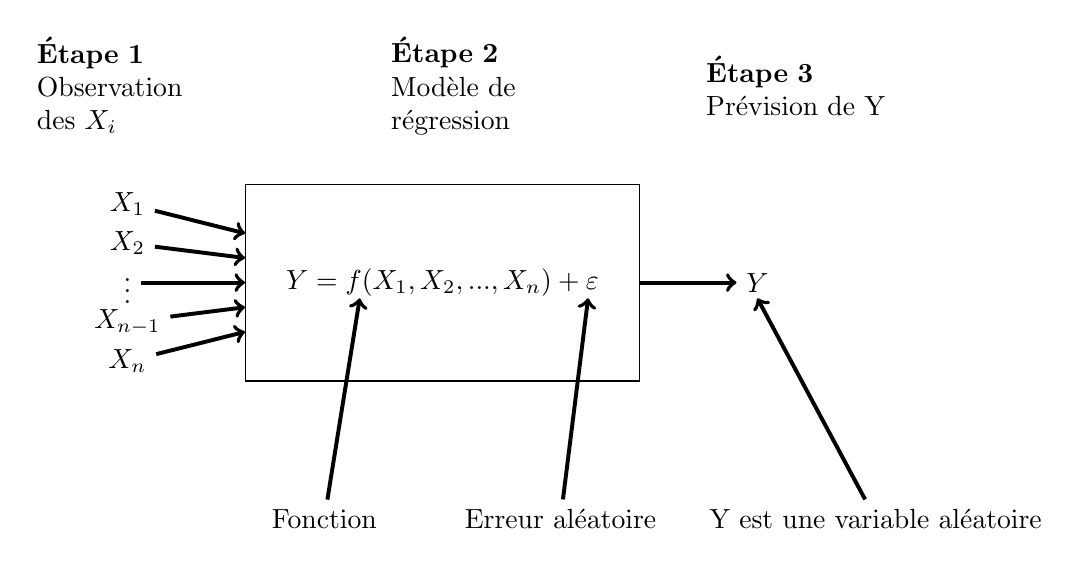
\begin{tikzpicture}
\node[block] (operator) at (4,1){$Y = f(X_1,X_2,...,X_n) + \varepsilon$};
\node[text width = 2.3cm] at (0,3.5) {\textbf{Étape 1} \\
									Observation des $X_i$};
\node[text width = 2.3cm] at (4.5,3.5) {\textbf{Étape 2} \\
									Modèle de régression};
\node[text width = 2.3cm] at (8.5,3.5) {\textbf{Étape 3} \\
									Prévision de Y};										
\node (a) at (0, 2) {$X_1$};
\draw[->, line width=0.5mm] ([right] a) --  (operator);
\node (b)at (0, 1.5) {$X_2$};
\draw[->, line width=0.5mm] ([right] b) --  (operator);
\node (c)at (0, 1) {$\vdots$};
\draw[->, line width=0.5mm] ([right] c) --  (operator);
\node (d)at (0, 0.5) {$X_{n-1}$};
\draw[->, line width=0.5mm] ([right] d) --  (operator);
\node (e)at (0, 0) {$X_{n}$};
\draw[->, line width=0.5mm] ([right] e) --  (operator);
\node (y)at (8, 1) {$Y$};
\draw[->, line width=0.5mm] (operator) -- ([left] y);
\node (F)at (2.5, -2) {Fonction};
\draw[->, line width=0.5mm] (F) --  (2.95, 0.8);
\node (E)at (5.5, -2) {Erreur aléatoire};
\draw[->, line width=0.5mm] (E) --  (5.85, 0.8);
\node (Y)at (9.5, -2) {Y est une variable aléatoire};
\draw[->, line width=0.5mm] (Y) --  (8, 0.8);
\end{tikzpicture}

\pagebreak

\subsection{Regression linéaire simple}
\label{sec:linsimple}

On cherche à prédire l'âge des passagers du Titanic selon le prix du billet à l'aide du modèle linéaire suivant,

\bigskip

%%% fig linéaire simple
\begin{center}
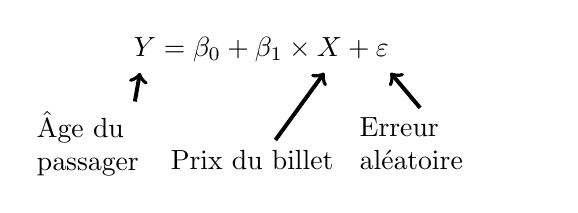
\begin{tikzpicture}[node distance=1.2cm]
\label{fig:linsimp}
\node (function) at (current page.center) {$Y  = \beta_0 + \beta_1 \times X + \varepsilon$};
\coordinate[below of=function] (c);
\node[text width = 2.3cm, left of=c, xshift=-0.5cm]  (Y) {Âge du passager};
\draw[->, line width=0.5mm] (Y) -- ([xshift=2mm, yshift=-3mm] function.west);
\node[text width = 2.3cm, below of=c, yshift=1cm] (X) {Prix du billet};
\draw[->, line width=0.5mm] (X) -- ([xshift=0.8cm, yshift=-3mm] function.center);
\node[text width = 2.3cm, right of=c, xshift=1.2cm] (E) {Erreur aléatoire};
\draw[->, line width=0.5mm] (E) -- ([xshift=-0.1cm, yshift=-3mm] function.east);
\end{tikzpicture}
\end{center}

%% Graphe modèle linéaire simple
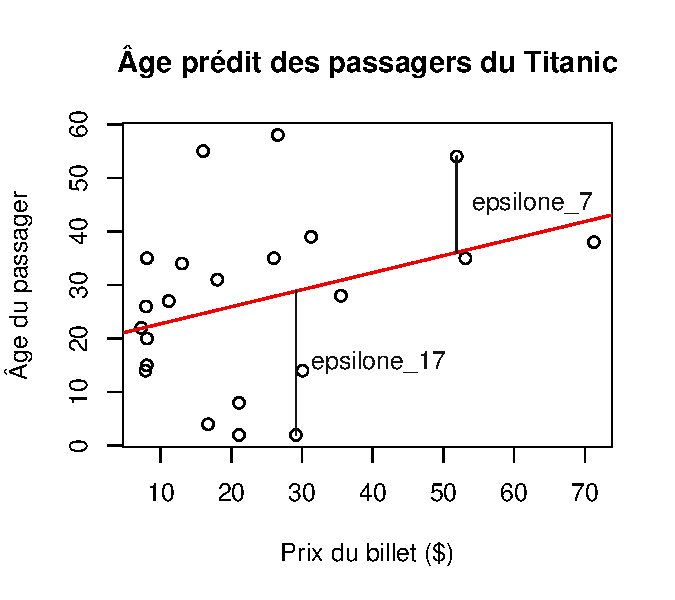
\includegraphics{notes_de_cours-001}

\subsection{Régression linéaire multiple}
\label{ex:multiple}
On cherche à prédire l'âge des passagers du Titanic selon le prix du billet et son sexe à l'aide du modèle linéaire suivant,

\bigskip

%%% fig linéaire multiples
\begin{center}
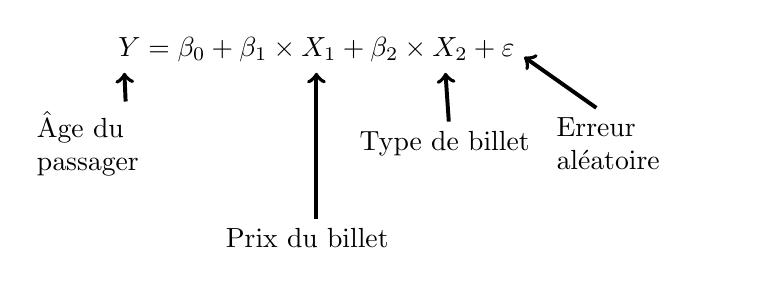
\begin{tikzpicture}[node distance=1.2cm]
\node (function) at (current page.center) {$Y  = \beta_0 + \beta_1 \times X_1 + \beta_2 \times X_2 + \varepsilon$};
\coordinate[below of=function] (c);
\node[text width = 2.3cm, left of=c, xshift=-1.2cm]  (Y) {Âge du passager};
\draw[->, line width=0.5mm] (Y) -- ([xshift=2mm, yshift=-3mm] function.west);
\node[text width = 2.3cm, below of=c, yshift=-0.0001cm] (X) {Prix du billet};
\draw[->, line width=0.5mm] (X) -- ([xshift=0cm, yshift=-3mm] function.center);
\node[text width = 2.3cm, right of=c, xshift=0.5cm] (X2) {Type de billet};
\draw[->, line width=0.5mm] (X2) -- ([xshift=-1cm, yshift=-3mm] function.east);
\node[text width = 2.3cm, right of=c, xshift=3cm] (E) {Erreur aléatoire};
\draw[->, line width=0.5mm] (E) -- ([ yshift=-1mm] function.east);
\end{tikzpicture}
\end{center}

%% fig 1 multilinear regression
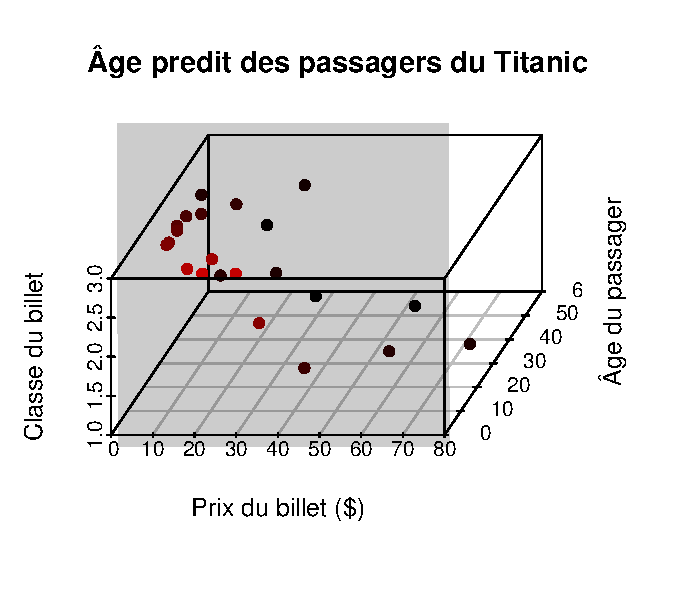
\includegraphics{notes_de_cours-002}

Voici la régression sous un autre angle, on voit la surface plane de régression.
%% fig 2
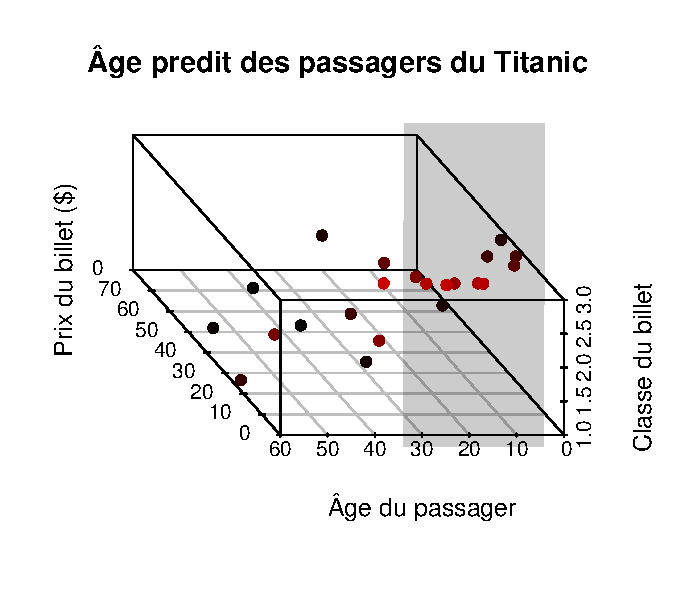
\includegraphics{notes_de_cours-003}

\subsection{Régression exponentielle}
On cherche à prédire la sévérité d'un sinistre automobile en fonction du temps à l'aide du modèle exponentiel suivant,

%%% fig exponentiel
\begin{center}
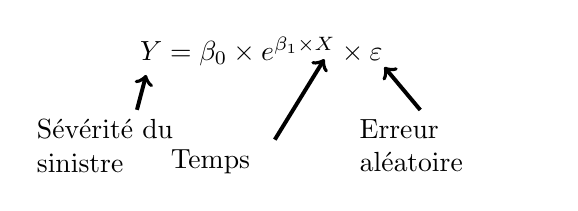
\begin{tikzpicture}[node distance=1.2cm]
\node (function) at (current page.center) {$Y  = \beta_0 \times  e^{\beta_1 \times X} \times \varepsilon$};
\coordinate[below of=function] (c);
\node[text width = 2.3cm, left of=c, xshift=-0.5cm]  (Y) {Sévérité du sinistre};
\draw[->, line width=0.5mm] (Y) -- ([xshift=2mm, yshift=-3mm] function.west);
\node[text width = 2.3cm, below of=c, yshift=1cm] (X) {Temps};
\draw[->, line width=0.5mm] (X) -- ([xshift=0.8cm, yshift=-1mm] function.center);
\node[text width = 2.3cm, right of=c, xshift=1.2cm] (E) {Erreur aléatoire};
\draw[->, line width=0.5mm] (E) -- ([xshift=-0.1cm, yshift=-2mm] function.east);
\end{tikzpicture}
\end{center}

%% Figure modèle exponentiel
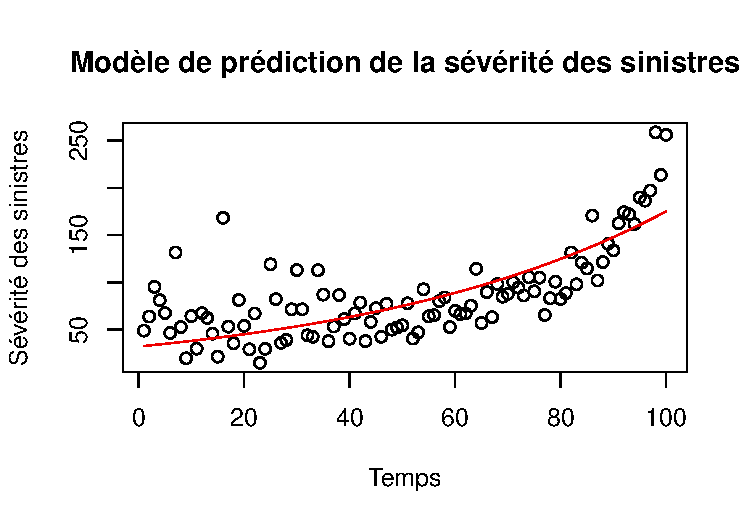
\includegraphics{notes_de_cours-004}


\subsubsection*{Note}
\label{note:exponentielle}
On remarque que la régression exponentielle est similaire à une régression linéaire simple.
\begin{align*}
\ln (Y) &= \ln (\beta_0) + \beta_1 \times X + \ln (\varepsilon) \\
Y^* &= \beta_0^* + \beta_1 \times X + \varepsilon^*\\
\end{align*}
Qu'on appelle aussi une régression multiplicative ou log linéaire.

\subsection{Régression quadratique}
On cherche à prédire la sévérité d'un sinistre automobile en fonction du temps et du temps au carré à l'aide du modèle quadratique suivant,

%%% fig quadratique
\begin{center}
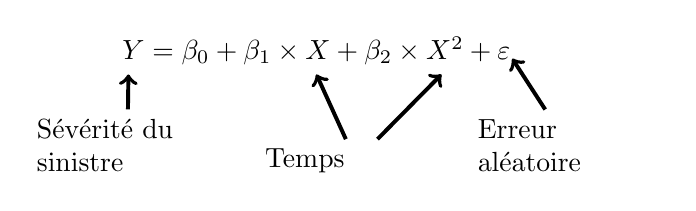
\begin{tikzpicture}[node distance=1.2cm]
\node (function) at (current page.center) {$Y  = \beta_0 + \beta_1 \times X + \beta_2 \times X^2 + \varepsilon$};
\coordinate[below of=function] (c);
\node[text width = 2.3cm, left of=c, xshift=-1.2cm]  (Y) {Sévérité du sinistre};
\draw[->, line width=0.5mm] (Y) -- ([xshift=2mm, yshift=-3mm] function.west);
\node[text width = 2.3cm, below of=c, yshift=1cm, xshift = 0.5cm] (X) {Temps};
\draw[->, line width=0.5mm] (X) -- ([xshift=0cm, yshift=-3mm] function.center);
\draw[->, line width=0.5mm] (X) -- ([xshift=-1cm, yshift=-3mm] function.east);
\node[text width = 2.3cm, right of=c, xshift=2cm] (E) {Erreur aléatoire};
\draw[->, line width=0.5mm] (E) -- ([yshift=-1mm, xshift = -1mm] function.east);
\end{tikzpicture}
\end{center}

%% Graphe modèle quadratique
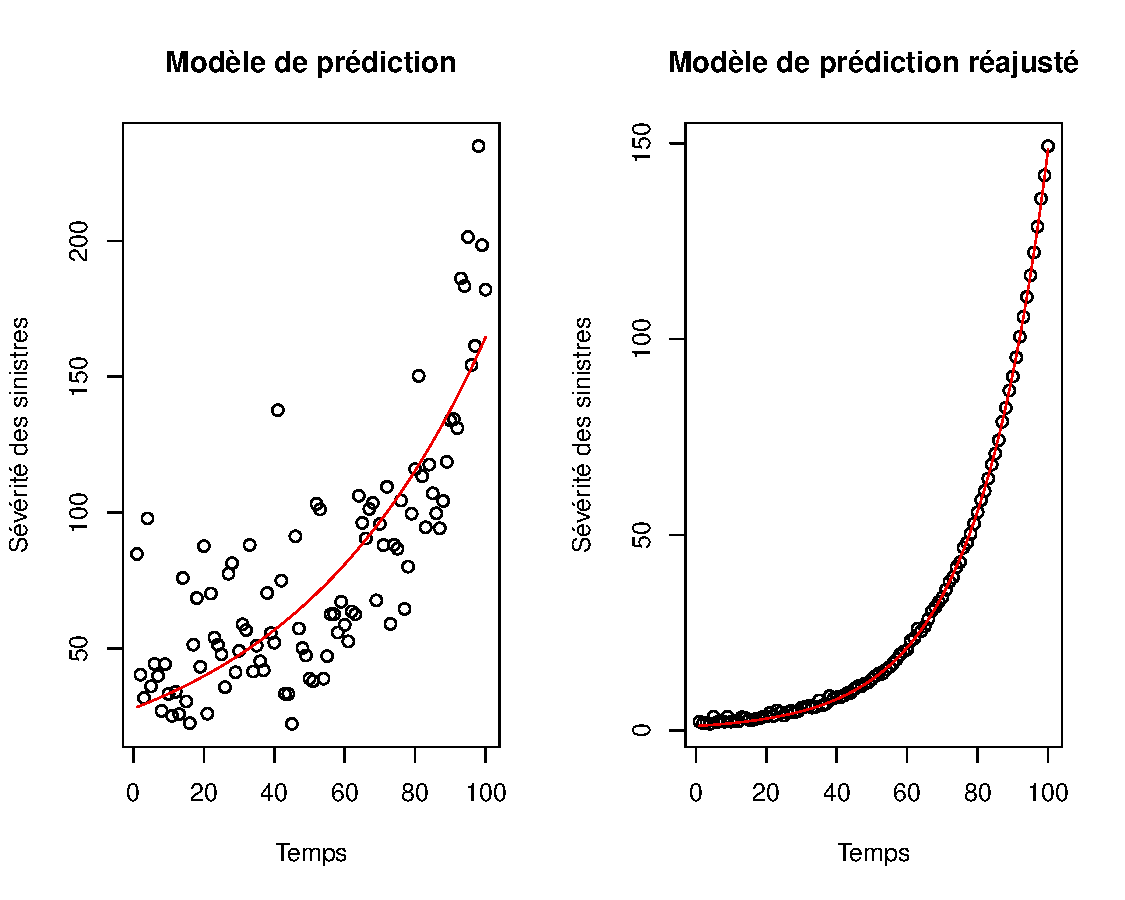
\includegraphics{notes_de_cours-005}

\subsubsection*{Note}
\label{note:quadratique}
On remarque que la régression quadratique est similaire à une régression linéaire multiple. En posant $X_1=X$ et $X_2 = X^2$
\begin{align*}
Y &= \beta_0 + \beta_1 \times X_1 + \beta_2 \times X_2 + \varepsilon\\
\end{align*}
Soit une régression linéaire multiple.

Dans le cadre du cours, seulement les modèles linéaires seront à l'étude pour les différentes raisons suivantes

\begin{itemize}
\item Plus simples
\item Plusieurs modèles peuvent se ramener à un modèle linéaire simple ou multiple. (voir \ref{note:exponentielle} et \ref{note:quadratique})
\item Constituent souvent une très bonne approximation de la réalité qui peut être très complexe, telle que l'assurance.
\item Se généralisent facilement, tels que les \textit{Generalized Linear Models}.
\end{itemize}

Le principal problème de la modélisation linéaire est de trouver les différents paramètres $\beta_0, \beta_1, ..., \beta_n$ de telle sorte que
\begin{equation}
\varepsilon = Y - f(X_1,...,X_n; \beta_0, \beta_1,...,\beta_n)
\end{equation}
soit minimisé.

Il existe plusieurs méthodes pour calcul l'erreur. Soit les erreurs suivantes :
\begin{itemize}
\item Erreur totale
\item Erreur absolue
\item Erreur quadratique
\end{itemize}

Quel type d'erreur est suffisante pour déterminer $\varepsilon$ ?

\subsubsection{Erreur totale}
\begin{equation}
\sum_{t=1}^n \varepsilon_t = \sum_{t=1}^n \Big( Y_t - (\beta_0 + \beta_1\times X_t) \Big) 
\end{equation}
\begin{itemize}
\item Facile à mettre à 0
\item Manque de fiabilité à cause de la mise à zéro
\end{itemize}

%% Graphe modèle quadratique
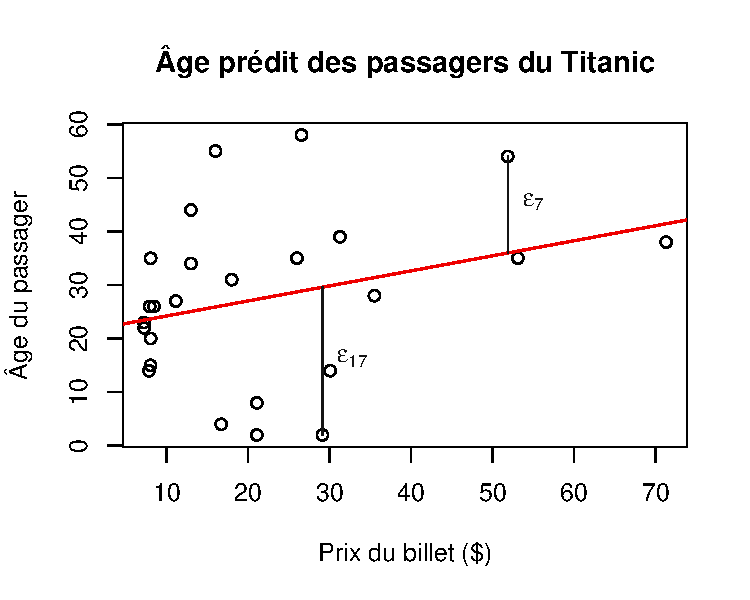
\includegraphics{notes_de_cours-006}

\subsubsection{Erreur absolue}
\begin{equation}
\sum_{t=1}^n |\varepsilon_t| = \sum_{t=1}^n \Big| Y_t - (\beta_0 + \beta_1\times X_t) \Big| 
\end{equation}
\begin{itemize}
\item Très robuste
\item Très compliquée mathématiquement, pour minimiser $\sum_{t=1}^n |\varepsilon_t|$ cela implique de dériver la fonction.
\end{itemize}

\subsubsection{Erreur quadratique}
\begin{equation}
\sum_{t=1}^n \varepsilon_t^2 = \sum_{t=1}^n \Big[ Y_t - (\beta_0 + \beta_1\times X_t) \Big]^2 
\end{equation}
\begin{itemize}
\item Mathématiquement plus simple que l'erreur absolue
\item Donne beaucoup de poids aux grandes erreurs
\end{itemize}

\bigskip
L'erreur quadratique semble donc l'option la plus simple due à la facilité mathématique et sa fiabilité.

\section{Le modèle de régression linéaire simple}
Le modèle de régression linéaire simple tente d'expliquer le mieux possible la variable \href{https://fr.wikipedia.org/wiki/Variable_dépendante}{dépendante} \footnote{On appelle parfois la variable dépendante une variable \href{https://fr.wikipedia.org/wiki/Endogène}{endogène}. Qui s'interprète comme étant une variable qui est due à une cause interne.}  Y à l'aide d'une variable \href{https://fr.wikipedia.org/wiki/Variable_indépendante}{indépendante}\footnote{On appelle parfois les variables dépendantes des variables \href{https://fr.wikipedia.org/wiki/Exogène}{exogène}. Qui s'intreprète comme étant extérieur à un système.} X . 

Si on dispose de n paires d'observations $(X_1, Y_1), (X_2, Y_2),...,(X_n, Y_n)$ alors, le modèle s'exprime  comme suit :
\begin{equation}
\label{eq:simple}
Y_i = \beta_0 + \beta_1\times X_i + \varepsilon_i \text{,  i = 1, ...,n.}
\end{equation}

Où $\beta_0$ est le paramètre associé à l'ordonnée à l'origine du modèle;
$\beta_1$ est le paramètre associé à la pente de la droite;
et $\varepsilon$ est le terme d'erreur.

\subsubsection*{Quelques remarques sur le modèle}
Dans l'équation \ref{eq:simple} du modèle, on remarque que :
\begin{itemize}
\item Les observations de $Y_i$ son tirées d'une variable aléatoire;
\item Les observations de $X_i$ sont considérées comme des valeurs connues et non aléatoires;
\item Les paramètres $\beta_0$ et $\beta_1$ sont inconnus au départ. Ils doivent être estimés;
\item $\varepsilon_i$ sont des réalisations inconnues d'une variable aléatoire.
\end{itemize}

\subsubsection*{Exemple d'un modèle de régression}
\begin{align*}
X_t &: \text{Nombre d'années de scolarité de l'actuaire} t \\
Y_t &: \text{Salaire de l'actuaire} t\\
\end{align*}

Comment résoudre le modèle pour prédire les salaires des actuaires en fonction du nombre d'années de scolarité ?

\bigskip
\textbf{Raisonnement:}
\begin{itemize}
\item Pour $X_t = 0$; on a $Y_t = \beta_0$. Autrement dit, le salaire avec un nombre d'années nulle de scolarité est \emph{en moyenne} de $\beta_0$. Par exemple, $\beta_0$ serait le salaire moyen d'un stagiaire.
\item Par la suite, pour chaque année additionnelle de scolarité, le salaire augmente \emph{en moyenne }de $\beta_1$ unitées.
\end{itemize}
Ainsi, \emph{en moyenne} on a 
\begin{align*}
E[Y_t|X_t] &= \beta_0 + \beta_1\times X_t
\end{align*}

Habituellement, la relation n'est pas parfaitement exacte dans la réalité. On se retrouve ainsi avec une \emph{différence} dans notre variable exogène prédite. L'erreur est notée $\varepsilon_t$ et est telle que mentionnée plus tôt, assumée aléatoire.
\begin{align*}
\varepsilon_t &= Y_t - E[Y_t|X_t] \\
&= Y_t - (\beta_0 + \beta_1\times X_t)\\
\end{align*}

En réorganisant, on retrouve l'équation \ref{eq:simple}.
%%% fig linéaire simple 2
\begin{center}
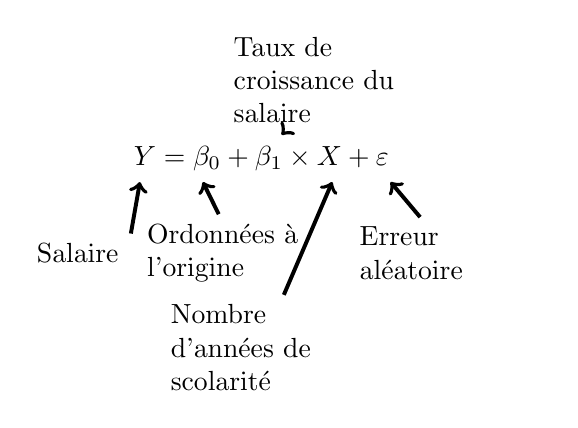
\begin{tikzpicture}[node distance=1.2cm]
\node (function) at (current page.center) {$Y  = \beta_0 + \beta_1 \times X + \varepsilon$};
\coordinate[below of=function] (c);
\node[text width = 2.3cm, left of=c, xshift=-0.5cm]  (Y) {Salaire};
\draw[->, line width=0.5mm] (Y) -- ([xshift=2mm, yshift=-3mm] function.west);
\node[text width = 2.3cm, left of=c, xshift=0.9cm]  (B) {Ordonnées à l'origine};
\draw[->, line width=0.5mm] (B) -- ([xshift=1cm, yshift=-3mm] function.west);
\node[text width = 2.5cm, above of=c, xshift=0.9cm, yshift=1cm]  (B2) {Taux de croissance du salaire};
\draw[->, line width=0.5mm] (B2) -- ([xshift=2cm, yshift=3mm] function.west);
\node[text width = 2.3cm, below of=c] (X) {Nombre d'années de scolarité};
\draw[->, line width=0.5mm] (X) -- ([xshift=0.9cm, yshift=-3mm] function.center);
\node[text width = 2.3cm, right of=c, xshift=1.2cm] (E) {Erreur aléatoire};
\draw[->, line width=0.5mm] (E) -- ([xshift=-0.1cm, yshift=-3mm] function.east);
\end{tikzpicture}
\end{center}

On doit maintenant trouver les paramètres $\beta_0$ et $\beta_1$ de manière à minimiser l'erreur $\varepsilon_t$.

Si $\varepsilon_t$ est minimal, cela veut dire que $Y_t \approx \beta_0 + \beta_1\times X_t$. Ce qui signifie que la droite de régression est une bonne approximation de $Y_t$.

\begin{moreInfo}{\emph{En résumé}}
	En résumé, on cherche à minimiser nos résidus en optimisant les paramètres $\beta_i$. 
\end{moreInfo}

\subsection{Coefficients de régression}
\label{subsec:coeffreg}
Les paramètres $\beta_0$ et $\beta_1$ sont déterminés en minimisant l'erreur quadratique à l'aide de la méthode des moindres carrés.

\begin{align*}
S(\beta_0, \beta_1) &= \sum_{t=1}^n \varepsilon_t^2 \\
&= \sum_{t=1}^n \big( Y_t - (\beta_0 + \beta_1\times X_t) \big)^2 \\
&= \sum_{t=1}^n \big( Y_t - \beta_0 - \beta_1\times X_t \big)^2 \\
\end{align*}

Où $S(\psi)$ peut être considérée comme une mesure de la \emph{distance} entre les données observées et le modèle théorique qui prédit ces données \footnote{Pour de plus amples informations sur la méthode des moindres carrés et la fonction de \emph{distance}, la page \href{https://fr.wikipedia.org/wiki/Méthode_des_moindres_carrés}{Wikipédia} contient une bonne explication sur le sujet.}.

\bigskip
Afin de minimiser la fonction $S(\beta_0, \beta_1)$, on dérive la fonction partiellement en fonction de chacun des paramètres.

\subsubsection*{Minimisation de $\beta_0$}
\begin{align*}
\frac{\partial S(\hat{\beta_0}, \hat{\beta_1})}{\partial \beta_0} &= 0 \\
\frac{\partial}{\partial \beta_0} \sum_{t=1}^n \big( Y_t - \hat{\beta_0} - \hat{\beta_1}\times X_t \big)^2 &= 0 \\
-2\sum_{t=1}^n \big( Y_t - \hat{\beta_0} - \hat{\beta_1} \times X_t \big) &= 0 \\
\end{align*}
\begin{equation}
\label{eq:minimisationbeta0}
\sum_{t=1}^n Y_t - n \times \hat{\beta_0} - \hat{\beta_1} \sum_{t=1}^n X_t = 0 \\
\end{equation}

\subsubsection*{Minimisation de $\beta_1$}
\begin{align*}
\frac{\partial S(\hat{\beta_0}, \hat{\beta_1})}{\partial \beta_1} &= 0 \\
\frac{\partial}{\partial \beta_1} \sum_{t=1}^n \big( Y_t - \hat{\beta_0} - \hat{\beta_1}\times X_t \big)^2 &= 0 \\
-2\sum_{t=1}^n \big( Y_t - \hat{\beta_0} - \hat{\beta_1} \times X_t \big) \times X_t &= 0 \\
\end{align*}
\begin{equation}
\label{eq:minimisationbeta1}
\sum_{t=1}^n Y_t \times X_t - \hat{\beta_0} \sum_{t=1}^n X_t - \hat{\beta_1} \sum_{t=1}^n X_t^2 = 0 \\
\end{equation}

À l'aide des équations \ref{eq:minimisationbeta0} et \ref{eq:minimisationbeta1}, on peut trouver les deux inconnus $\beta_0$ et $\beta_1$.

À partir de \ref{eq:minimisationbeta0} :

\begin{align*}
\sum_{t=1}^n Y_t - n \times \hat{\beta_0} - \hat{\beta_1} \sum_{t=1}^n X_t &= 0 \\
\sum_{t=1}^n Y_t - \hat{\beta_1} \sum_{t=1}^n X_t &=  n \times \hat{\beta_0} \\
\frac{\sum_{t=1}^n Y_t}{n} - \hat{\beta_1} \frac{\sum_{t=1}^n X_t}{n} &=  \hat{\beta_0} \\
\end{align*}

\begin{equation}
\label{eq:beta0}
\color{blue}
\boxed{\color{black}
\hat{\beta_0} = \overline{Y} - \hat{\beta_1} \overline{X}}
\end{equation}

Et à partir de \ref{eq:minimisationbeta1} :

\begin{align*}
\sum_{t=1}^n Y_t \times X_t - \hat{\beta_0} \sum_{t=1}^n X_t - \hat{\beta_1} \sum_{t=1}^n X_t^2 &= 0 \\
\sum_{t=1}^n Y_t \times X_t - \hat{\beta_0} \sum_{t=1}^n X_t &=  \hat{\beta_1} \sum_{t=1}^n X_t^2 \\
\end{align*}

\begin{equation}
\label{eq:beta}
\hat{\beta_1} =  \frac{\sum_{t=1}^n Y_t \times X_t - \hat{\beta_0} \sum_{t=1}^n X_t}{\sum_{t=1}^n X_t^2}
\end{equation}

On utilise l'équation \ref{eq:beta0} de $\hat{\beta_0}$ avec l'équation \ref{eq:beta} de $\hat{\beta_1}$, on développe l'équation résultante afin d'isoler $\hat{\beta_1}$.

\begin{align*}
\hat{\beta_1} &= \frac{\sum_{t=1}^n Y_t \times X_t - (\overline{Y} - \hat{\beta_1}\overline{X})\sum_{t=1}^n X_t}{\sum_{t=1}^n X_t^2} \\
&= \frac{\sum_{t=1}^n Y_t \times X_t - (\overline{Y} - \hat{\beta_1}\overline{X})\times n \overline{X}}{\sum_{t=1}^n X_t^2} \\
&= \frac{\sum_{t=1}^n Y_t X_t - n\overline{Y}\overline{X} + \hat{\beta_1}\times \overline{X}^2 \times n}{\sum_{t=1}^n X_t^2} \\
\end{align*}
En isolant $\hat{\beta}_1$, on obtient la définition suivante

\begin{equation}
\label{eq:beta1}
\color{blue}
\boxed{\color{black}
\hat{\beta_1} = \frac{\sum_{t=1}^n Y_t X_t - n\overline{Y}\overline{X}}{\sum_{t=1}^n X_t^2 - n\overline{X}^2}
}
\end{equation}

\subsubsection*{Remarques}

\begin{enumerate}
\item On note $\hat{\varepsilon}_t$ les résidus générés par le modèle estimé:
\begin{align*}
\hat{\varepsilon}_t &= Y_t - \hat{Y}_t \\
\hat{\varepsilon}_t &= Y_t - (\hat{\beta}_0 - \hat{\beta}_1 X_t) \text{; pour t = 1,2,...,n} \\
\end{align*}

Si on illustre graphiquement les résidus, il s'agit du segment le plus court entre la droite de régression et la donnée observée. 

\bigskip
Si on reprend le graphique de la section \ref{fig:linsimp}, on observe facilement les résidus sur cette représentation graphique :

%% Graphe modèle linéaire simple
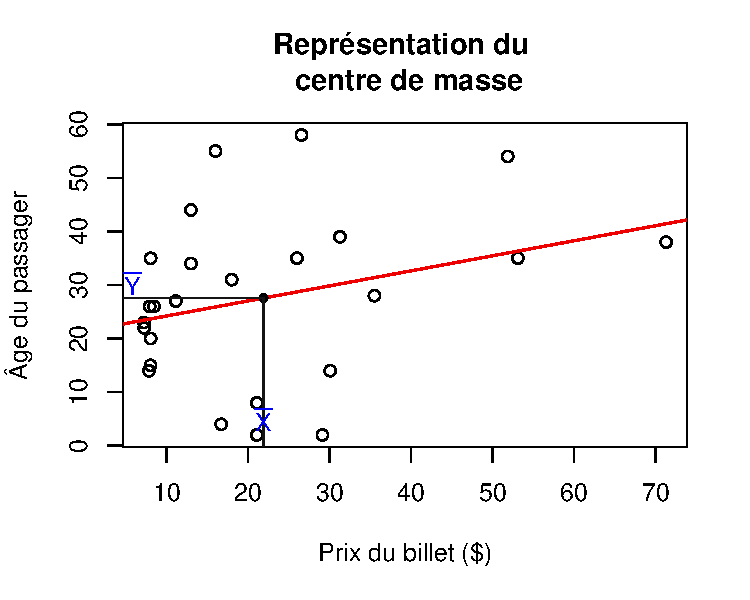
\includegraphics{notes_de_cours-007}

\item Le \emph{centre de gravité}\footnote{Qu'on appelle parfois le centre de masse.} des données $(\overline{X}, \overline{Y})$ se trouvent exactement sur la droite de régression.

On peut facilement effectuer cette preuve à partir de l'équation \ref{eq:beta0},
\begin{align*}
\hat{\beta_0} &= \overline{Y} - \hat{\beta_1} \overline{X} \\
\overline{Y} &=  \hat{\beta_0} + \hat{\beta_1} \overline{X} + 0 \\
\end{align*}
On note ainsi une absence de résidus pour le centre de masse.

\bigskip
Si on reprend (encore) le graphique de la section \ref{fig:linsimp}, on observe facilement le centre de masse sur le graphique. 

%% Graphe modèle Xbarre et Ybarre
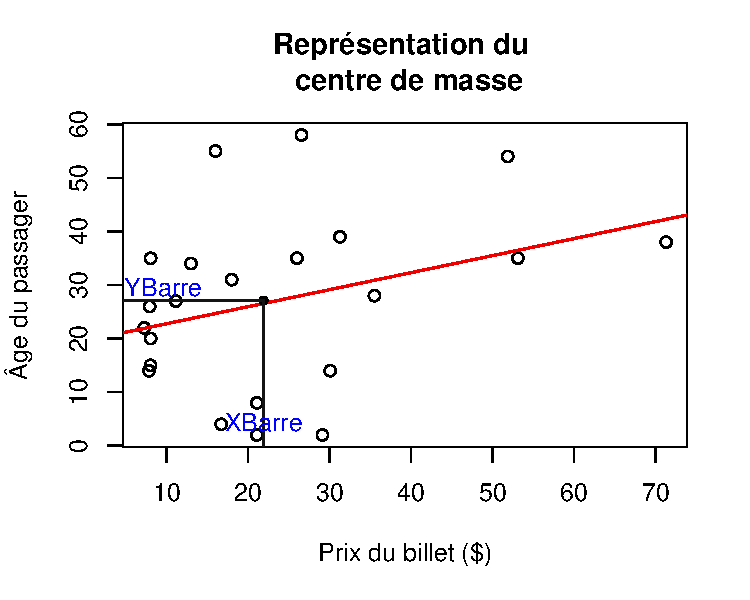
\includegraphics{notes_de_cours-008}

\item La somme des résidus de tout modèle de régression linéaire est nulle.
\begin{align*}
\sum_{t=1}^{n} \hat{\varepsilon}_t &= \sum_{t=1}^{n}\big( Y_t - (\hat{\beta}_0 + \hat{\beta}_1 X_t) \big) \\
&\overset{\ref{eq:beta0}}{=} \sum_{t=1}^{n}\big( Y_t - (\overline{Y} - \hat{\beta}_1 \overline{X}) \big) \\
&= \sum_{t=1}^{n} Y_t - \sum_{t=1}^{n}\overline{Y} + \hat{\beta}_1 \sum_{t=1}^{n}\overline{X} - \hat{\beta}_1\sum_{t=1}^{n}X_t \\
&= n \overline{Y} - n \overline{Y} + \hat{\beta}_1 + n \overline{X} - \hat{\beta}_1 + n \overline{X} \\
&= 0
\end{align*}
\end{enumerate}

\subsubsection*{Notation}
Afin de faciliter l'écriture, on intègre la notation suivante; $S_{xx}$ et  $S_{xy}$. Les expressions précédantes sont appelées respectivement: la somme des carrés corrigée de $x$ et la somme des produits croisés corrigée de $x$ et de $y$.
Voici le développement pour $S_{xx}$,
\begin{align*}
S_{xx} &= \sum_{t=1}^n (X_t - \overline{X})^2 \\
&= \sum_{t=1}^n (X_t - \overline{X})^2 \\
&= \sum_{t=1}^n (X_t^2 - 2X_t\overline{X} + \overline{X}^2) \\
&= \sum_{t=1}^n X_t^2 - 2\overline{X}\sum_{t=1}^n X_t + n\overline{X}^2 \\
&= \sum_{t=1}^n X_t^2 - 2\overline{X}n\overline{X} + n\overline{X}^2 \\
&= \sum_{t=1}^n X_t^2 - n\overline{X}^2 \\
\end{align*}

On effectue le même type de développement pour $S_{xy}$, 
\begin{align*}
S_{xy} &= \sum_{t=1}^n (X_t - \overline{X}) (Y_t - \overline{Y}) \\
&\vdots \\
&= \sum_{t=1}^n X_tY_t - n\overline{X}\overline{Y}\\
\end{align*}

À l'aide des sommes de carrés corrigés, on peut réécrire la définition de $\hat{\beta}_1$

%% beta_1 en fonction de Sxx et Sxy
\begin{equation}
\label{eq:beta1SXY}
\color{blue}
\boxed{\color{black}
\hat{\beta_1} = \frac{S_{xy}}{S_{xx}}
}
\end{equation}

\bigskip
\subsubsection*{Exemple}
\label{exemple1}
On poursuit avec un exemple pour assimiler l'information.

\bigskip
\begin{description}
\item[•] On dispose des cinq observations suivantes du couple $(X_t, Y_t)$ dans le tableau de gauche ainsi que les éléments calculés nécessaires pour trouver les paramètres dans le tableau de droite.
\end{description}

\begin{minipage}[t]{.4\linewidth}
\begin{tabular}{|c|c|c|}
\hline
t & $X_t$ & $Y_t$ \\
\hline
1 & 2 & 2 \\
2 & 3 & 5 \\
3 & 6 & 3 \\
4 & 9 & 6 \\
5 & 12 & 5 \\
\hline
Totaux : & 32 & 21 \\
\hline
\end{tabular}
\end{minipage}
\hfill
\begin{minipage}[t]{.4\linewidth}
\begin{tabular}{|c|c|c|}
\hline
t & $X_t^2$ & $X_tY_t$ \\
\hline
1 & 4 & 4 \\
2 & 9 & 15 \\
3 & 36 & 18 \\
4 & 81 & 54 \\
5 & 144 & 60 \\
\hline
Totaux : & 274 & 151 \\
\hline
\end{tabular}
\end{minipage}

\bigskip
%%calcul
À partir des définitions \ref{eq:beta0} et  \ref{eq:beta1}, on trouve facilement la valeur de $\hat{\beta}_0$ et de $\hat{\beta}_1$.

\begin{align*}
\hat{\beta_1} &= \frac{\sum_{t=1}^n Y_t X_t - n\overline{Y}\overline{X}}{\sum_{t=1}^n X_t^2 - n\overline{X}^2} \\
&= \frac{151 - (5)(\frac{21}{5})(\frac{32}{5})}{274 - (5)(\frac{32}{5})^2} \\
&= \frac{83}{346} \\
& \approx 0.2399 \\
\end{align*}

\begin{align*}
\hat{\beta_0} &= \overline{Y} - \hat{\beta_1} \overline{X} \\
&= \frac{21}{5} - (\frac{83}{346}) \times (\frac{32}{5}) \\
& \approx 2.6647
\end{align*}

On obtient ainsi le modèle de régression suivant :
\begin{align*}
Y_t &= 2.6647 + 0.2399X_t + \varepsilon_t
\end{align*}

\begin{center}
\begin{tabular}{|c|c|c|}
\hline
t & $Y_t = \hat{\beta}_0 + \hat{\beta}_1X_t$ & $\hat{\varepsilon}_t$ \\
\hline
1 & 3.1445 & -1.1445 \\
2 & 3.3844 & 1.6156 \\
3 & 4.1041 & -1.1041 \\
4 & 4.8238 & 1.1762 \\
5 & 5.5435 & -0.5435 \\
\hline
\end{tabular}
\end{center}

\begin{center}
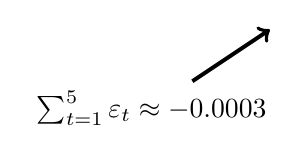
\begin{tikzpicture}[node distance=1.2cm]
\node (E) at (10,0) {$\sum_{t=1}^{5}\varepsilon_t \approx -0.0003$};
\draw[->, line width=0.5mm] (E) -- (11.5,1);
\end{tikzpicture}
\end{center}

\bigskip
\subsubsection*{Exécution en R}
%% script R
\begin{lstlisting}[linerange=\\begin\{Sinput\}-\\end\{Sinput\},includerangemarker=false, caption = Code source en R pour l'exemple]
\begin{Schunk}
\begin{Sinput}
> # Dataset
> x <- c(2,3,6,9,12); y <- c(2,5,3,6,5)
> # Estimations des parametres
> reg <- lm(y ~ x)
> # Resume de l'estimation
> summary(reg)
> # Valeurs de Yt
> fitted(reg)
> # Residus 
> residuals(reg)
\end{Sinput}
\end{Schunk}
\end{lstlisting}

\bigskip
%% info bull astuce calculatrice + reférence vers le guide
\begin{moreInfo}{\emph{Astuce calculatrice}}
	La calculatrice TI-30XS Multiview permet de créer un tableau de donnée et de sortir rapidement et facilement différentes informations sur une régression à partir des données. Tel que :
	\begin{itemize}
	\item $\overline{X}$ et $\overline{Y}$ ;
	\item $\sum_{t=1}^n X_t$, $\sum_{t=1}^n X_t^2$, $\sum_{t=1}^n Y_t$, $\sum_{t=1}^n Y_t^2$ et $\sum_{t=1}^n X_tY_t$ ;
	\item $\hat{\beta}_0$ et $\hat{\beta}_1$
	\end{itemize}
	Pour de plus ample information, consulter le \href{https://github.com/alpa12/guide_calculatrice}{guide} sur les calculatrices.
\end{moreInfo}
\bigskip

\subsection{Caractéristiques du terme d'erreur}
On rappelle que l'équation du modèle de régression correspond à 

\begin{align*}
Y_t &= \beta_0 + \beta_1\times X_t + \varepsilon_t \text{ (\ref{eq:simple})}
\end{align*}
De plus, on sait qu'il s'agit des valeurs moyennes de $Y_t$ en sachant $X_t$, soit
\begin{align*}
Y_t = E[Y_t|X_t] + \varepsilon_t 
\end{align*}

On peut ainsi formuler les trois postulats \footnote{Le \href{https://fr.wikipedia.org/wiki/Postulat}{postulat} est un principe non démontré, mais utilisé dans la construction d'une théorie mathématique. } suivants,
\begin{enumerate}
\item \label{post1} $E[\varepsilon_t] = 0$, par définition pour que $E[Y_t] = E[Y_t|X_t]$. Il s'agit de l'hypothèse de linéarité de la variable explicative. On dit qu'elle est exogène si elle n'est pas corrélée au terme d'erreur.
\item \label{post2} $Var(\varepsilon_t) = \sigma^2$, la variance des termes d'erreurs est supposée constante. Il s'agit de l'hypothèse d'homoscédasticité.
\item \label{post3} $Cov(\varepsilon_t, \varepsilon_s) = 0$, pour $t \neq s$,il n'y a pas de corrélation entre les termes d'erreurs. Il s'agit de l'hypothèse d'indépendance des erreurs.
\end{enumerate}

\bigskip
%% info bull hypothèse implicite
\begin{moreInfo}{\emph{Quatrième postulat}}
\label{post4}
	Les hypothèses de linéarité et d'homoscédasticité sont très intéressantes, si on observe leurs définitions ensemble on remarque qu'il s'agit d'une distribution avec une espérance nulle et une variabilité supposée constante. Ce qui nous amène à une quatrième hypothèse, les résidus sont distribués selon une loi normale.
	\begin{align*}
\hat{\varepsilon}_t|x_i \sim N(0, \sigma^2)
	\end{align*}
\end{moreInfo}
\bigskip

\section{Propriétés de l'estimateur des moindres carrés (EMC)}
\label{sec:EMC}

\subsection{Estimateur sans biais}
On rappelle qu'un estimateur est dit sans biais lorsque son espérance est égale à la valeur vraie du paramètre, soit $E[\hat{\theta}] = \theta \Leftrightarrow b(\hat{\theta}) = 0$ \footnote{Notes de cours ACT-2000, chapitre 3, Thomas Landry, Hiver 2017.}.

\begin{align*}
E[\hat{\beta}_1] &= E \Bigg[ \frac{\sum_{t=1}^n(X_t- \overline{X})(Y_t - \overline{Y})}{\sum_{t=1}^n(X_t - \overline{X})^2} \Bigg] \\
&= \frac{\sum_{t=1}^n(X_t- \overline{X})E[Y_t - \overline{Y}]}{\sum_{t=1}^n(X_t - \overline{X})^2} \\
&= \frac{\sum_{t=1}^n(X_t- \overline{X})(E[Y_t] - E[\overline{Y}])}{\sum_{t=1}^n(X_t - \overline{X})^2} \\
\end{align*}
De l'équation \ref{eq:simple}, et avec le postulat \ref{post1}, on sait que,

\begin{align*}
Y_t &= \beta_0 + \beta_1\times X_t + \varepsilon_t \\
E[Y_t] &= E[\beta_0 + \beta_1\times X_t] + E[\varepsilon_t] \\
&\overset{\ref{post1}}{=} \beta_0 + \beta_1\times X_t + 0 \\
\end{align*}
On applique le même raisonnement pour l'espérance de $\overline{Y}$. 

\begin{align*}
E[\hat{\beta}_1] &= \frac{\sum_{t=1}^n(X_t- \overline{X})(E[Y_t] - E[\overline{Y}])}{\sum_{t=1}^n(X_t - \overline{X})^2} \\
&= \frac{\sum_{t=1}^n(X_t- \overline{X})(\beta_0 + \beta_1\times X_t - \beta_0 - \beta_1\overline{X_t})}{\sum_{t=1}^n(X_t - \overline{X})^2} \\
&= \frac{\sum_{t=1}^n(X_t- \overline{X})\beta_1 (X_t - \overline{X_t})}{\sum_{t=1}^n(X_t - \overline{X})^2} \\
&= \beta_1 \frac{\sum_{t=1}^n(X_t- \overline{X})^2}{\sum_{t=1}^n(X_t - \overline{X})^2} \\
E[\hat{\beta}_1] &= \beta_1
\end{align*}
\bigskip

Par conséquent,
\begin{align*}
E[\hat{\beta}_0] &= E[\overline{Y} - \hat{\beta}_1 \overline{X}] \\
&= E[\overline{Y}] - \overline{X} E[\hat{\beta}_1]  \\
&= \beta_0 + \beta_1\overline{X} - \overline{X}\beta_1 \\
E[\hat{\beta}_0]  &= \beta_0 \\
\end{align*}

On peut ainsi conclure que les deux estimateurs des paramètres sont sans biais.

\subsection{Variances et covariances des estimateurs}
On s'intéresse aux variances et aux covariances des estimateurs, cette deuxième propriété ainsi que la première nous permettera de déduire une conclusion en lien avec le quatrième postulat.

\begin{align*}
Var(\hat{\beta}_1) &= Var\Bigg( \frac{\sum_{t=1}^n(X_t- \overline{X})(Y_t - \overline{Y})}{\sum_{t=1}^n(X_t - \overline{X})^2} \Bigg)\\
&= \frac{Var\big( \sum_{t=1}^n(X_t- \overline{X})Y_t - \sum_{t=1}^n(X_t- \overline{X} \big)\overline{Y}\big)}{\big( \sum_{t=1}^n(X_t - \overline{X})^2 \big)^2} \\
&= \frac{Var\big( \sum_{t=1}^n(X_t- \overline{X})Y_t\big) + Var\big(\sum_{t=1}^n(X_t- \overline{X})\overline{Y}\big)}{\big( \sum_{t=1}^n(X_t - \overline{X})^2 \big)^2} \\
&= \frac{\sum_{t=1}^n(X_t- \overline{X})^2 Var(Y_t) + Var\big(\overline{Y}(n\overline{X}- n\overline{X})\big)}{\big( \sum_{t=1}^n(X_t - \overline{X})^2 \big)^2} \\
&= \frac{\sum_{t=1}^n(X_t- \overline{X})^2 Var(\beta_0 + \beta_1X_t + \varepsilon_t) + 0}{\big( \sum_{t=1}^n(X_t - \overline{X})^2 \big)^2} \\
\end{align*}

\begin{center}
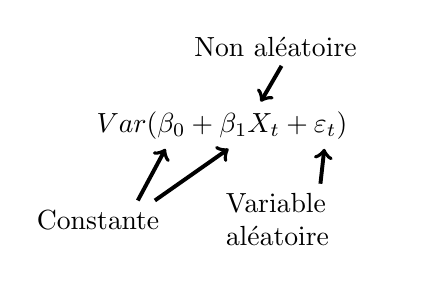
\begin{tikzpicture}[node distance=1.2cm]
\node (function) at (current page.center) {$Var(\beta_0 + \beta_1X_t + \varepsilon_t)$};
\coordinate[below of=function] (c);
\node[text width = 2.3cm, left of=c]  (Y) {Constante};
\draw[->, line width=0.5mm] (Y) -- ([xshift=1cm, yshift=-3mm] function.west);
\draw[->, line width=0.5mm] (Y) -- ([xshift=1.8cm, yshift=-3mm] function.west);
\node[text width = 2.5cm, above of=c, xshift=0.9cm, yshift=1cm]  (B2) {Non aléatoire};
\draw[->, line width=0.5mm] (B2) -- ([xshift=2.21cm, yshift=3mm] function.west);
\node[text width = 2.3cm, right of=c] (X) {Variable aléatoire};
\draw[->, line width=0.5mm] (X) -- ([xshift=1.3cm, yshift=-3mm] function.center);
\end{tikzpicture}
\end{center}

\begin{align*}
&= \frac{\sum_{t=1}^n(X_t- \overline{X})^2 Var(\varepsilon_t)}{\big( \sum_{t=1}^n(X_t - \overline{X})^2 \big)^2} \\
& \overset{\ref{post2}}{=} \frac{\sum_{t=1}^n(X_t- \overline{X})^2 \sigma^2}{\big( \sum_{t=1}^n(X_t - \overline{X})^2 \big)^2} \\
\end{align*}

\begin{equation}
\label{eq:varbeta1}
\color{blue}
\boxed{\color{black}
Var(\hat{\beta_1}) = \frac{\sigma^2}{\sum_{t=1}^n(X_t - \overline{X})^2}}
\end{equation}

\begin{align*}
Var(\hat{\beta}_0) &= Var(\overline{Y} - \hat{\beta}_1\overline{X})\\
&= Var(\overline{Y}) + Var(\hat{\beta}_1\overline{X}) -  2 Cov(\overline{Y}, \hat{\beta}_1\overline{X}) \\
&= Var\Big(\frac{\sum_{t=1}^n Y_t}{n} \Big) + \overline{X}^2 Var(\hat{\beta}_1) -  2 \overline{X} Cov(\overline{Y}, \hat{\beta}_1) \\
&= \frac{n \times Var(Y_t)}{n^2}  + \overline{X}^2 \Bigg(\frac{\sigma^2}{\sum_{t=1}^n (X_t - \overline{X})^2}\Bigg) -  2 \overline{X} Cov(\overline{Y}, \hat{\beta}_1) \\
\end{align*}

\begin{align*}
Cov(\overline{Y}, \hat{\beta}_1) &= Cov \Bigg( \frac{\sum_{t=1}^n Y_t}{n}, \frac{\sum_{s=1}^n(X_s- \overline{X})(Y_s - \overline{Y})}{\sum_{s=1}^n(X_s - \overline{X})^2} \Bigg) \\
&= \frac{1}{n}\frac{1}{\sum_{s=1}^n(X_s - \overline{X})^2} Cov\Bigg(\sum_{t=1}^n Y_t, \sum_{s=1}^n(X_s- \overline{X})Y_s - \overline{Y}\sum_{s=1}^n(X_s- \overline{X}) \Bigg) \\
&= \frac{1}{n}\frac{1}{\sum_{s=1}^n(X_s - \overline{X})^2} \sum_{t=1}^n \sum_{s=1}^n (X_s- \overline{X}) Cov(Y_t, Y_s) \\
&= \frac{1}{n}\frac{1}{\sum_{s=1}^n(X_s - \overline{X})^2} \Bigg( \mathop{\sum_{t=1}^n \sum_{s=1}^n}_{:t \neq s} (X_s- \overline{X}) \times 0 + \mathop{\sum_{t=1}^n \sum_{s=1}^n}_{:t = s} (X_s- \overline{X}) \sigma^2 \Bigg) \\
&= \frac{1}{n}\frac{1}{\sum_{s=1}^n(X_s - \overline{X})^2}\sigma^2 \bigg( \sum_{t=1}^n (X_t - \overline{X}) \bigg) \\
&= \frac{1}{n}\frac{1}{\sum_{s=1}^n(X_s - \overline{X})^2}\sigma^2 (n\overline{X}- n\overline{X}) \\
&= 0
\end{align*}

\begin{equation}
\label{eq:varbeta0}
\color{blue}
\boxed{\color{black}
Var(\hat{\beta}_0) = \frac{\sigma^2}{n}  + \overline{X}^2 \bigg(\frac{\sigma^2}{\sum_{t=1}^n (X_t - \overline{X})^2}\bigg)}
\end{equation}

Finalement, pour la covariance entre $\hat{\beta}_0$ et $\hat{\beta}_1$
\begin{align*}
Cov(\hat{\beta}_0, \hat{\beta}_1) &= Cov(\overline{Y} - \hat{\beta}_1\overline{X}, \hat{\beta}_1) \\
&= Cov(\overline{Y},  \hat{\beta}_1) - \overline{X} Var(\hat{\beta}_1) \\
&= 0 - \overline{X} \frac{\sigma^2}{\sum_{t=1}^n (X_t - \overline{X})^2} \\
\end{align*}

\begin{equation}
\label{eq:covariance}
\color{blue}
\boxed{\color{black}
Cov(\hat{\beta}_0, \hat{\beta}_1) = - \overline{X} \frac{\sigma^2}{\sum_{t=1}^n (X_t - \overline{X})^2}}
\end{equation}

\bigskip
%% info bull postulat 4 et param.
\begin{moreInfo}{\emph{Résumé des propriétés des estimateurs}}
\label{res:estima}
	Les équations \ref{eq:varbeta0} et \ref{eq:varbeta1}  ainsi que le postulat 4 à la section \ref{post4} nous permettent de conclure que 
	\begin{align*}
	     \hat{\beta_0} &\sim N\Bigg(\beta_0, \frac{\sigma^2}{n}  + \overline{X}^2 \bigg(\frac{\sigma^2}{\sum_{t=1}^n (X_t - \overline{X})^2}\bigg)\Bigg) \\
	     \hat{\beta_1} &\sim N\Bigg(\beta_1, \frac{\sigma^2}{\sum_{t=1}^n(X_t - \overline{X})^2})\Bigg)
	\end{align*}

\end{moreInfo}
\bigskip

\subsection{Optimalité}
Le théorème de \href{https://fr.wikipedia.org/wiki/Théorème_de_Gauss-Markov}{Gauss-Markor} nous permet d'établit que l'estimateur des moindres carrés est l'estimateur non biaisé à variance minimale. 

\subsubsection*{Notions importantes à retenir du théorème:}
\begin{enumerate}
\item Considérer l'estimateur $\Theta^* = \sum_{t=1}^n C_t \times Y_t$
\item Minimiser $Var(\Theta^*)$ sous la contrainte que $E[\Theta^*] = \beta$; où
$$ \beta =
\begin{bmatrix}
  \beta_0 \\
  \beta_1 \\ 
\end{bmatrix} $$
\end{enumerate}

\section{Régression passant par l'origine}
Dans certaines situations, il est possible que l'on souhaite forcer la droite de régression à passer par l'origine.
Voici un exemple de situation où il est plus logique de forcer le modèle,
\begin{align*}
X_t &: \text{Nombre de Km parcouru} t \\
Y_t &: \text{Consommation d'essence en L d'une voiture} t\\
\end{align*}
Il est plus logique d'avoir une consommation de 0 L pour une distance de 0 Km.

Dans ce cas, on peut postuler le modèle suivant :
\begin{equation}
\label{eq:regzero}
Y_t = \beta \times X_t + \varepsilon_t
\end{equation}

On peut démontrer par le même raisonnement qu'à la section \ref{subsec:coeffreg} que de minimisation du paramètre $\beta$ correspond à :

\begin{equation}
\label{eq:betasimp}
\color{blue}
\boxed{\color{black}
\hat{\beta} = \frac{\sum_{t=1}^n X_t Y_t}{\sum_{t=1}^n X_t^2}}
\end{equation}

On reprend l'exemple énoncer plus haut, voici le modèle représenter graphiquement :
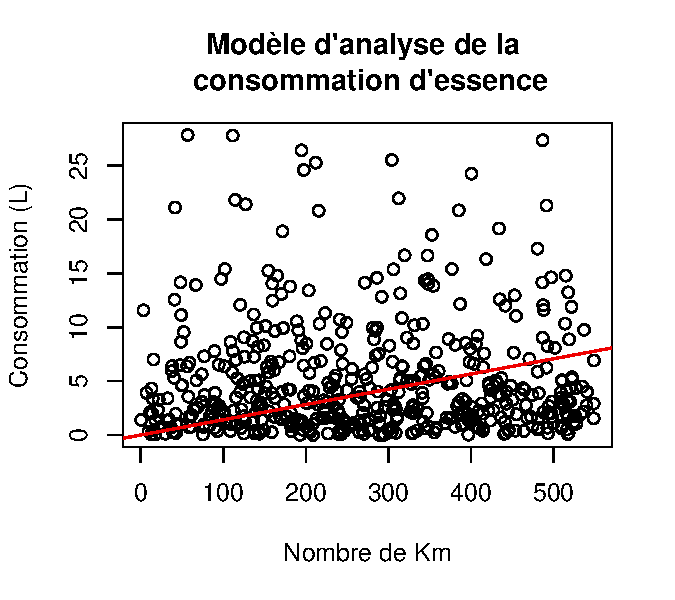
\includegraphics{notes_de_cours-010}

\subsubsection*{Code R}
Voici le code R permettant de créer un modèle linéaire simple avec une droite passant par l'origine.

\begin{lstlisting}[linerange=\\begin\{Sinput\}-\\end\{Sinput\},includerangemarker=false, caption = Code source en R pour l'exemple]
\begin{Schunk}
\begin{Sinput}
> # dataset
> # X Km parcourus
> # Y consommation essence en L
> simul <- 500
> alpha <- 1
> beta <- alpha/5.1
> y <- rgamma(simul, alpha, beta)
> x <- runif(simul, 0, 550)
> # Estimation de beta
> reg <- lm(y ~ x - 1)
> plot(x, y, xlab = "Nombre de Km", ylab = "Consommation (L)", main= "Modele d'analyse de la \n consommation d'essence")
> abline(reg, col="red2", lwd = 1.5)
\end{Sinput}
\end{Schunk}
\end{lstlisting}
\bigskip

\section{Analyse de la variance}
\label{sec:anaVar}
Un tableau d'analyse de la variance permet d'évaluer la qualité de l'ajustement du modèle aux observations.

\subsubsection*{Idée}
\begin{enumerate}
\item Si on décide de modéliser $Y_t$ sans la régression, autrement dit de l'analyse statistique \footnote{Cours ACT-2000}, alors $Y$ est vue comme une variable aléatoire avec une certaine variance, soit $Var(y)$.
\item En utilisant la régression pour modéliser $Y_t$ en fonction de $X_t$ une partie de la variance de $Y_t$ est \emph{expliquée} par la variance de $X_t$, alors que l'autre partie reste \emph{inexpliquée}.
\item L'utilité de la régression est de trouver la proportion de la variance de $Y_t$ qui est expliquée par la variance de $X_t$.
\end{enumerate}

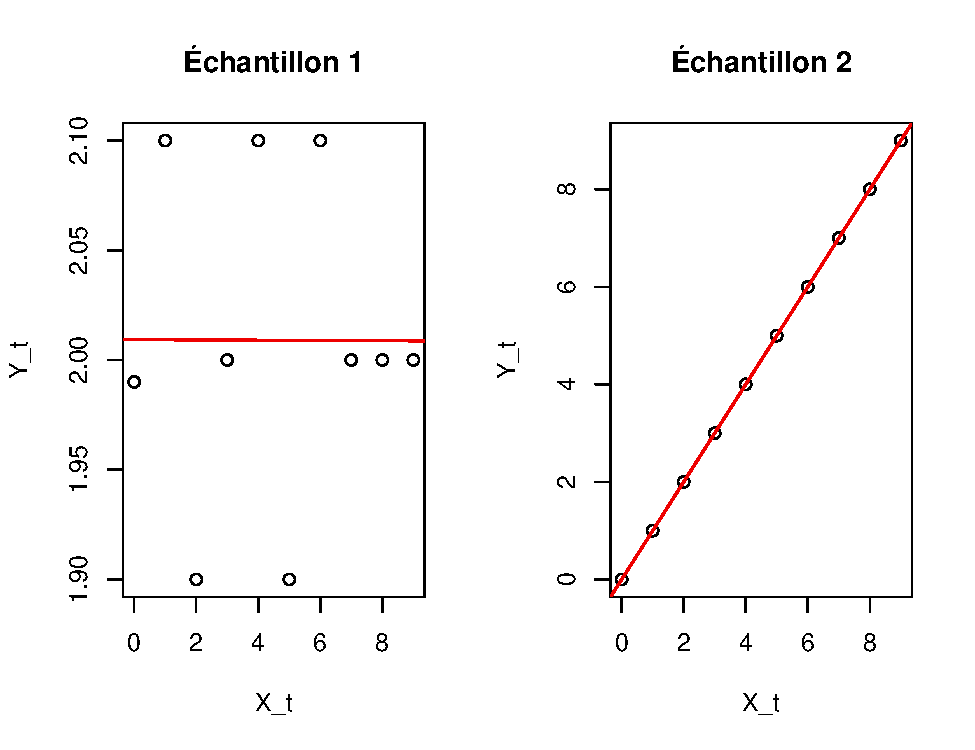
\includegraphics{notes_de_cours-012}

On voit que les résidus de l'échantillon 1 sont très mal expliqués par notre modèle, les résidus sont très élevés. Tandis que les résidus de l'échantillon 2 sont parfaitement expliqués par notre modèle.
\begin{Schunk}
\begin{Soutput}
$residusMauvaisFit
       1        2        3        4        5        6        7        8 
2.009273 2.009212 2.009152 2.009091 2.009030 2.008970 2.008909 2.008848 
       9       10 
2.008788 2.008727 
\end{Soutput}
\begin{Soutput}
$residusBonFit
            1             2             3             4             5 
-2.580003e-16  1.000000e+00  2.000000e+00  3.000000e+00  4.000000e+00 
            6             7             8             9            10 
 5.000000e+00  6.000000e+00  7.000000e+00  8.000000e+00  9.000000e+00 
\end{Soutput}
\end{Schunk}

Il y a peu d'intérêt de construire un modèle avec les données de l'échantillon 1 car,

\begin{center}
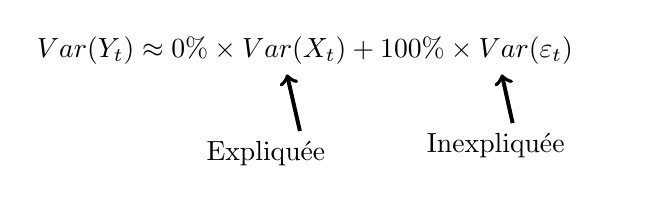
\begin{tikzpicture}[node distance=1.2cm]
\node (function) at (current page.center) {$Var(Y_t) \approx 0\% \times Var(X_t) + 100\% \times Var(\varepsilon_t)$};
\coordinate[below of=function] (c);
\node[text width = 2.5cm, below of=c, yshift = 1.1cm]  (B2) {Expliquée};
\draw[->, line width=0.5mm] (B2) -- ([xshift=3.3cm, yshift=-3mm] function.west);
\node[text width = 2.3cm, right of=c, xshift = 1.5cm] (X) {Inexpliquée};
\draw[->, line width=0.5mm] (X) -- ([xshift=2.5cm, yshift=-3mm] function.center);
\end{tikzpicture}
\end{center}
Il est préférable dans ce cas-ci d'utiliser les modèles statistiques vus dans le cours ACT-2000.

\bigskip
Par contre, il y a un intérêt à utiliser un modèle avec les données de l'échantillon 2 car,
$$
Var(Y_t) = Var(X_t)
$$
Autrement dit, la variable X explique bien la variable Y.

\subsubsection*{Note}
Noter que les modèles précédents  ont été ajustés pour mieux représenter le concept, un modèle avec un fit parfait n'est pas réaliste dans la réalité.

\subsection{Notions préliminaires : Somme des carrés}
La variance totale de $Y_t$ est décomposable sous le modèle de régression linéaire, cette décomposition permet d'analyser l'ajustement du modèle. On la représente ainsi :
$$
SST = \sum_{t=1}^n(Y_t-\overline{Y})^2
$$
\bigskip
\subsubsection*{Décomposition}
\begin{align*}
(Y_t - \overline{Y}) &= Y_t - \hat{Y}_t + \hat{Y}_t - \overline{Y} \\
(Y_t - \overline{Y}) &= (Y_t - \hat{Y}_t) + (\hat{Y}_t - \overline{Y}) \\
\end{align*}

\begin{center}
\begin{tabularx}{\textwidth}{XXX}
$\underbrace{(Y_t - \overline{Y}) =} $ & $\underbrace{(Y_t - \hat{Y}_t) \  +}$ & $\underbrace{(\hat{Y}_t - \overline{Y})}$ \\
Variation totale de $Y_t$ & Variation de $Y_t$ & Résidu \\
& Variation expliquée \newline par la régression & Variation inexpliquée \newline par la régression \\
\end{tabularx}
\end{center}

%% figure représentation des variations
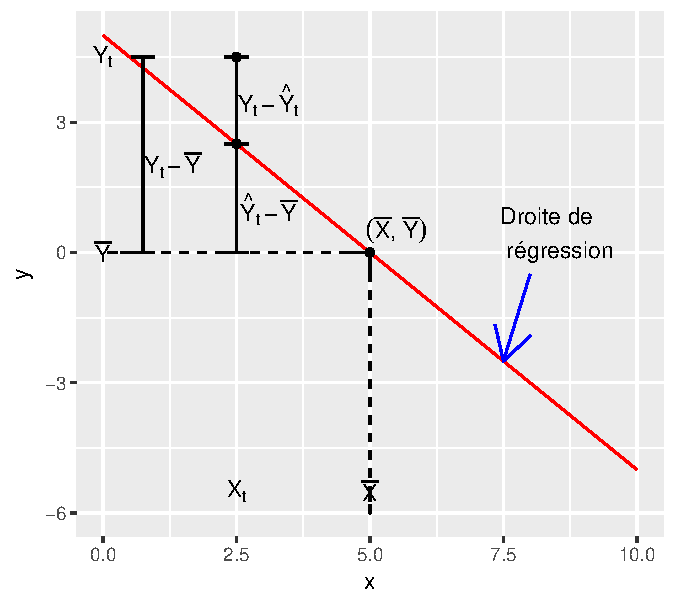
\includegraphics{notes_de_cours-014}

Par conséquent, on a que
\begin{align*}
SST &= \sum_{t=1}^n \bigg[ (\hat{Y_t} - \overline{Y}) + (Y_t - \hat{Y}_t) \bigg]^2 \\
&= \sum_{t=1}^n (\hat{Y_t} - \overline{Y})^2 + \sum_{t=1}^n(Y_t - \hat{Y}_t)^2 + 2 \sum_{t=1}^n (\hat{Y_t} - \overline{Y})(Y_t - \hat{Y}_t)\\
\end{align*}
\begin{center}
\begin{tabular}{cccc}
 = & $\underbrace{\sum_{t=1}^n (\hat{Y_t} - \overline{Y})^2 \  + }$ & $\underbrace{\sum_{t=1}^n(Y_t - \hat{Y}_t)^2 \  +} $ & $\underbrace{2 \sum_{t=1}^n (\hat{Y_t} - \overline{Y})(Y_t - \hat{Y}_t)}$\\
 & SSR & SSE & $\psi$ \\
 & Régression & Erreur & \\
\end{tabular}
\end{center}

\subsubsection*{Développement de $\psi$}
\begin{align*}
2 \sum_{t=1}^n (\hat{Y_t} - \overline{Y})(Y_t - \hat{Y}_t) &\Rightarrow 2 \sum_{t=1}^n (\hat{\beta}_0 + \hat{\beta}_1X_t - \hat{\beta}_0 - \hat{\beta}_1\overline{X})(Y_t - \overline{Y} + \overline{Y} - \hat{Y}_t) \\
&= 2 \sum_{t=1}^n \hat{\beta}_1 (\hat{X_t} - \overline{X}) (Y_t - \overline{Y} + \hat{\beta}_0 + \hat{\beta}_1\overline{X} - \hat{\beta}_0 - \hat{\beta}_1 X_t) \\
&= 2 \sum_{t=1}^n \hat{\beta}_1 (\hat{X_t} - \overline{X}) \bigg((Y_t - \overline{Y}) - \hat{\beta}_1(X_t - \overline{X}) \bigg)\\
&= 2 \hat{\beta}_1 \sum_{t=1}^n  (\hat{X_t} - \overline{X})(Y_t - \overline{Y}) - 2 \hat{\beta}_1^2 \sum_{t=1}^n (X_t - \overline{X})^2\\
&= 2 \hat{\beta}_1 (S_{xy} - \hat{\beta}_1S_{xx})\\
& \overset{\ref{eq:beta1SXY}}{=} 2 \hat{\beta}_1 (S_{xy} - \frac{S_{xy}}{S_{xx}}S_{xx})\\
&= 2 \hat{\beta}_1 (S_{xy} - S_{xy})\\
&= 0 \\
\end{align*}

Ainsi, 

\begin{equation}
\label{eq:SST}
\color{blue}
\boxed{\color{black}
\text{SST} = \text{SSR} + \text{SSE}}
\end{equation}
Où SSR est la variation expliquée par le modèle de régression linéaire et SSE signifie la variation inexpliquée, ou résiduelle du modèle de régression linéaire.
\bigskip

Intuitivement, 
\begin{itemize}
     \item Dans un bon modèle de régression, on aimerait que 
          \begin{itemize}
          \item $SST \approx SSR$, soit que $Var(Y_t) \approx Var(X_t)$ 
          \item[ou]
          \item $SSE \approx 0$, soit que la variation résiduelle soit très faible
          \end{itemize}
     \item On définit le coefficient de détermination par
          \begin{itemize}
          
          \item[]\begin{equation}
          \label{eq:R}
          \color{blue}
          \boxed{\color{black}
          R^2 = Corr^2(Y, \hat{Y}) = \frac{\text{SSR}}{\text{SST}} \Leftrightarrow 1 - \frac{\text{SSE}}{\text{SST}}}
          \end{equation}
          Par rapport au ratio, $\frac{\text{SSR}}{\text{SST}}$ signifie le pourcentage de la variance dans $Y_t$ expliqué par la régression et 
          $1 - \frac{\text{SSR}}{\text{SST}}$ signifie le pourcentage de la variance dans $Y_t$ qui n'est pas expliquée par la régression.
          \item $R^2 \in [0,1] $
          \item Si $R^2 = 100 \%$, la régression est parfaite et utile; si$R^2 = 0 \%$, la régression n'est pas parfaite et est inutile.
          \end{itemize}
\end{itemize}

\subsection{Notions préliminaires : Degrés de liberté}
Le nombre de \emph{degrés de liberté}\footnote{Couramment l'abréviation $d.l.$ sera utiliser pour signifié \emph{degrés de liberté}.} d'une \emph{somme de carrés} est :
\begin{itemize}
     \item Le nombre de composants \emph{indépendants} dans la somme ;
     \item[ou]
     \item Le nombre minimal de fonctions de $Y_1, ..., Y_n$ qu'il faut connaitre pour obtenir la somme ;
     \item[ou]
     \item \textbf{Pour $SST$ et $SSE$ seulement}
     $$
     \text{d.l.} = \Big( \text{Nombre de termes dans la somme}\Big) - \Big( \text{Nombre de paramètres estimés dans cette somme}\Big)
     $$
\end{itemize}

Ainsi, 
\begin{itemize}
\item $SST = \sum_{t=1}^n(Y_t-\overline{Y})^2 \rightarrow$ n termes - (1 paramètre estimé\footnote{$\overline{Y}$}) $= \color{blue}\boxed{\color{black} (n-1)d.l.}$
\item $SSE = \sum_{t=1}^n(Y_t - \hat{Y}_t)^2 $
$$
\sum_{t=1}^n(Y_t - \hat{Y}_t)^2 = \sum_{t=1}^n(Y_t - \hat{\beta}_0 - \hat{\beta}_1X_t )^2
\rightarrow \text{ n termes } - (\text{2 paramètres estimé}\footnote{$\hat{\beta}_0 \text{ et } \hat{\beta}_1$}) = \color{blue}\boxed{\color{black} (n-2)d.l.}
$$
\item $SSR = \sum_{t=1}^n (\hat{Y_t} - \overline{Y})^2 $
\begin{align*}
\sum_{t=1}^n (\hat{Y_t} - \overline{Y})^2 &= \sum_{t=1}^n(\hat{\beta}_0 + \hat{\beta}_1X_t - \hat{\beta}_0 - \hat{\beta}_1\overline{X})^2 \\
&= \underbrace{\hat{\beta}_1^2} \times \underbrace{\sum_{t=1}^n(X_t - \overline{X})^2} \\
 f&(y_1,...y_n) \  f(x_1,...,x_n)
\end{align*}
Soit une seule fonction des $Y_1,...,Y_n$ doit être connue pour obtenir $SSR \rightarrow  \color{blue}\boxed{\color{black} 1 \  d.l.}$ 
\end{itemize}

\subsubsection*{Remarque}
On sait que :
$$
SST = SSE + SSR
$$
On note aussi que 
\begin{align*}
d.l.(SST) &= d.l.(SSE) + d.l.(SSR) \\
(n-1) &= (n-2) + (1)
\end{align*}
On aurait donc pu retrouver $d.l.(SST) = d.l.(SSE) + d.l.(SSR)$

\subsection{Tableau d'analyse de la variance}
\label{seq:anova}
On appelle couramment le tableau d'analyse de la variance le tableau ANOVA. Ce type de tableau est utilisé dans tous les logiciels de régression pour évaluer la qualité d'un modèle.

\bigskip
\begin{tabularx}{\linewidth}{|X|X|X|X|X|}
\hline
Source de la variance & Somme des carrés $(SS)$ & Degrés de liberté $(d.l.)$ & Carrés moyens $(MS)$ & Ratio de Fisher $(F)$ \\
\hline
Régression & $SSR$ & 1 & $MSR = \frac{SSR}{1}$ & $F = \frac{MSR}{MSE}$ \\
Erreur & $SSE$ & n - 2 & $ MSE = \frac{SSE}{n-2}$ & \\
\hline
Total & $SST$ & n - 1 & & \\
\hline
\end{tabularx}

\bigskip
\subsubsection*{Exemple}
On poursuit avec un exemple pour assimiler l'information, on reprend l'exemple de la section \ref{exemple1}.

\bigskip
\begin{center}
\begin{tabular}{|c|c|c|c|c|}
\hline
t & $X_t$ & $Y_t$  & $\hat{Y}_t = \hat{\beta}_0 + \hat{\beta}_1X_t$ & $\hat{\varepsilon}_t$\\
\hline
1 & 2 & 2 & 3.1445 & -1.1445\\
2 & 3 & 5 & 3.3844 & 1.6156\\
3 & 6 & 3 & 4.1041 & -1.1041\\
4 & 9 & 6 & 4.8238 & 1.1762\\
5 & 12 & 5 & 5.5435 & -0.5435\\
\hline
Totaux : & 32 & 21 & & \\
\hline
\end{tabular}
\end{center}

\begin{align*}
SSE &= \sum_{t=1}^n (Y_t - \hat{Y}_t)^2 = \sum_{t=1}^n \varepsilon_t^2 = 6.8179 \\
SSR &= \sum_{t=1}^n (\hat{Y_t} - \overline{Y})^2 = 3.9821 \\
SST &= SSE + SSR = 6.8179 +3.9821 = 10.8000 \\
\end{align*}

\subsubsection*{ANOVA}
\begin{center}
\begin{tabular}{|c|c|c|c|c|}
\hline
Source & $SS$ & $d.l.$ & $MS$ & $F$ \\
\hline
Régression & 3.9821 & 1 & 3.9821 & 1.7522 \\
Erreur & 6.8179 & 3 & 2.2726 & \\
\hline
Totaux & 10.8000 & 4 & & \\
\hline
\end{tabular}
\end{center}

\subsubsection*{$R^2$}
\begin{align*}
R^2 &= \frac{SSR}{SST} = \frac{3.9821}{10.8000} = 36.87 \% \\
R^2 &= 1 - \frac{SSE}{SST} = 1 - \frac{6.8179}{10.8000} = 36.87 \% \\
\end{align*}
Autrement dit, seulement 36.87 \% de la variabilité des $Y_t$ est expliquée par la variabilité des $X_t$. La régression n'est pas très efficace et utile.

\subsubsection*{Code R}
Voici le code R permettant de créer un modèle linéaire simple avec une droite passant par l'origine.

\begin{lstlisting}[linerange=\\begin\{Sinput\}-\\end\{Sinput\},includerangemarker=false, caption = Code source en R pour l'exemple]
\begin{Schunk}
\begin{Sinput}
> # Dataset
> y <- c(2, 5, 3, 6, 5); x <- c(2, 3, 6, 9, 12)
> # Estimation des betas
> reg <- lm(y ~ x)
> anova(reg)
\end{Sinput}
\end{Schunk}
\end{lstlisting}
\bigskip

%%%%%%%%%%%%%% ANOVA CALCULATRICE ??? ASTUCE

\section{Intervalles de confiance (I.C.) et test d'hypothèses}
On poursuit l'objectif des sections \ref{sec:EMC} et \ref{sec:anaVar}m soit de valider la qualité du modèle de régression.

\subsection{Distribution des variables aléatoires}
\label{sec:distri}
On rappel qu'avec le postulat 4 (\ref{post4}), on suppose que les résidus suivent une loi normale d'espérance nulle et de variance de $\sigma^2$.
	\begin{align*}
\hat{\varepsilon}_t|x_i \overset{i.i.d.}{\sim} N(0, \sigma^2)
	\end{align*}

Les conséquences de ce postulat sont les suivantes :
\begin{enumerate}
\item $(Y_t = \beta_0 + \beta_1X_t + \varepsilon_t) \sim N(\beta_0 + \beta_1X_t, \sigma^2)$ (Postulat \ref{post1})
\item Les propriétés de l'estimateur des moindres carrés avaient permis de démontrer que (section \ref{sec:EMC}) :
	\begin{align*}
	     \hat{\beta_0} &\sim N\Bigg(\beta_0, \frac{\sigma^2}{n}  + \overline{X}^2 \bigg(\frac{\sigma^2}{\sum_{t=1}^n (X_t - \overline{X})^2}\bigg)\Bigg) \\
	     \hat{\beta_1} &\sim N\Bigg(\beta_1, \frac{\sigma^2}{\sum_{t=1}^n(X_t - \overline{X})^2})\Bigg)
	\end{align*}
	
\begin{moreInfo}{\emph{Alternative}}
	On peut tirer la même conclusion à partir de la propriété des fonctions linéaires de $\hat{\beta}_0$ et $\hat{\beta}_1$.
\end{moreInfo}

\item L'estimateur sans biais pour $\sigma^2$ est :
\begin{align*}
\sigma^2 &= S^2 = MSE \\
MSE &= \frac{SSE}{d.l.(SSE)} \\
\frac{SSE}{d.l.(SSE)} &= \frac{\sum_{t=1}^n (Y_t - \hat{Y}_t)^2}{n-2} \\
\end{align*}

\begin{equation}
\label{eq:s2}
\color{blue}
\boxed{\color{black}
\sigma^2 = \frac{\sum_{t=1}^n \varepsilon_t^2}{n-2}}
\end{equation}

\item On peut montrer que 
\begin{equation}
\label{eq:ssesigma}
\color{blue}
\boxed{\color{black}
\bigg(\frac{SSE}{\sigma^2}\bigg) \sim \chi^2(n - 2) }
\end{equation}
\end{enumerate}

\subsection{Intervalle de confiance pour $\beta_1$}
Attention de ne pas confondre avec $\hat{\beta}_1$.
\bigskip
Puisque $ \hat{\beta}_1 \sim N(\beta_1, Var(\hat{\beta}_1))$, on a que 
$$
\Bigg(\frac{\hat{\beta}_1 - \beta_1}{\sqrt{Var(\hat{\beta}_1)}}\Bigg) \sim N(0,1)
$$

Si $\sigma^2$ était connu, l'intervalle de confiance serait de la forme suivante 
$$
\bigg[\hat{\beta}_1\pm Z_{\alpha/2} \times \sqrt{Var(\hat{\beta}_1)}\bigg]
$$
Par contre, $\sigma^2$ n'est  souvent pas connu et il est nécessaire de l'estimer. Tel que mentionné plus haut, l'estimateur non biaisé correspond à l'équation \ref{eq:s2}. Mais cet estimateur ne suit pas une distribution normale. À l'aide des notions acquises en ACT-2000, il est possible de démontrer que si on utilise l'estimateur de $\sigma^2$, soit $S^2$, dans la formule de $Var(\hat{\beta}_1)$, c'est-à-dire :
$$
\widehat{Var}(\hat{\beta}_1) = \frac{S^2}{\sum_{t=1}^n (X_t - \overline{X})^2}
$$
Alors, on peut conclure que :
$$
\Bigg(\frac{\hat{\beta}_1 - \beta_1}{\sqrt{Var(\hat{\beta}_1)}}\Bigg) \sim t(n-2)
$$

On obtient ainsi l'intervalle de confiance suivant au niveau $100 \times (1 - \alpha)\%$ pour $\beta_1$ ,

\begin{equation}
\label{eq:intconfb1}
\color{blue}
\boxed{\color{black}
\hat{\beta}_1 \pm t_{\frac{\alpha}{2}}(n-2) \times \sqrt{\frac{S^2}{\sum_{t=1}^n (X_t - \overline{X})^2}}}
\end{equation}

\subsection{Intervalle de confiance pour $\beta_0$}
De manière similaire, un intervalle de confiance au niveau $100 \times (1 - \alpha)\%$ pour $\beta_0$ est,

\begin{equation}
\label{eq:intconfb0}
\color{blue}
\boxed{\color{black}
\hat{\beta}_0 \pm t_{\frac{\alpha}{2}}(n-2) \times \sqrt{\frac{S^2}{n} + \frac{S^2\overline{X}^2}{\sum_{t=1}^n (X_t - \overline{X})^2}}}
\end{equation}

\subsection{Test d'hypothèses sur les paramètres}
Principales questions auxquelles on aimerait répondre :
\begin{enumerate}
\item \label{hyp1} L'ordonnée à l'origine $(\beta_0)$ est-elle significativement différente de 0 ? \newline
Sinon, on considère le modèle $Y_t = \beta_1\times X_t + \varepsilon_t$.
\item  \label{hyp2} La pente $(\beta_1)$ est-elle significativement différente de 0 ? \newline
Sinon, on considère le modèle $Y_t = \beta_0 + \varepsilon_t$.
\end{enumerate}

Pour tester la question \ref{hyp1} :
\begin{align*}
H_0 &: \beta_0 = 0 \\
H_1 &: \beta_0 \neq 0 \\
&\text{On utilise la statistique suivante, } \\
t &= \frac{\hat{\beta}_0 - 0 }{\sqrt{\widehat{Var}(\hat{\beta}_0)}}
\end{align*}

Pour tester la question  \ref{hyp2} :

\begin{align*}
H_0 &: \beta_1 = 0 \\
H_1 &: \beta_1 \neq 0 \\
&\text{On utilise la statistique suivante, } \\
t &= \frac{\hat{\beta}_1 - 0 }{\sqrt{\widehat{Var}(\hat{\beta}_1)}}
\end{align*}

On rejette $H_0$ au niveau de confiance $100 \times (1 - \alpha)\%$ pour $\beta_0$ si :
$$
|t| > t_{\frac{\alpha}{2}(n-2)}
$$

Voici une représentation graphique de la zone de rejet bilatéral :

%% Figure zone de rejet bilateral
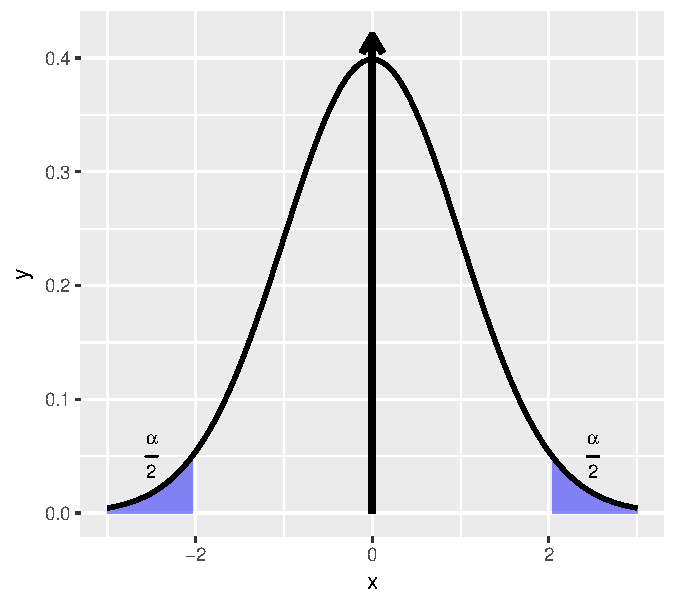
\includegraphics{notes_de_cours-016}

Qui correspond à la probabilité de \emph{se tromper} en rejetant $H_0$.

\subsubsection*{Remarques}
De manière générale, on utilise plutôt les tests d'hypothèses suivants pour nos deux questions:

Pour tester la question \ref{hyp1} :
\begin{align*}
H_0 &: \beta_0 = \beta_0^* \\
H_1 &: \beta_0 \neq \beta_0^* \\
&\text{On utilise la statistique suivante, } \\
t &= \frac{\hat{\beta}_0 - \beta_0^* }{\sqrt{\widehat{Var}(\hat{\beta}_0)}}
\end{align*}

Pour tester la question  \ref{hyp2} :

\begin{align*}
H_0 &: \beta_1 = \beta_1^* \\
H_1 &: \beta_1 \neq \beta_1^* \\
&\text{On utilise la statistique suivante, } \\
t &= \frac{\hat{\beta}_1 - \beta_1^* }{\sqrt{\widehat{Var}(\hat{\beta}_1)}}
\end{align*}

On rejette $H_0$ au niveau de confiance $100 \times (1 - \alpha)\%$ pour $\beta_0$ si :
$$
|t| > t_{\frac{\alpha}{2}(n-2)}
$$

\bigskip
On poursuit avec un exemple pour assimiler l'information.

\subsubsection*{Exemple}
Dans une régression sur un ensemble de 14 observations, on a obtenu :
$$
\hat{Y}_t = 68.494 - 0.468X_t
$$
ainsi que 
\begin{align*}
\widehat{Var}(\hat{\beta}) &= \widehat{Var}\Bigg(
\begin{bmatrix}
  \beta_0 \\
  \beta_1 \\ 
\end{bmatrix}\Bigg) \\
&= 
\begin{bmatrix}
  \widehat{Var}(\hat{\beta}_0) & \widehat{Cov}(\hat{\beta}_0, \hat{\beta}_1)\\
  \widehat{Cov}(\hat{\beta}_0, \hat{\beta}_1)  & \widehat{Var}(\hat{\beta}_1)\\ 
\end{bmatrix} \\
&= 
\begin{bmatrix}
  66.8511 & 1.2544\\
  1.2544 & 0.0237\\ 
\end{bmatrix} \\
\end{align*}

\subsubsection*{Question 1}
Tester si $\beta_0$ est significativement différent de 0 à un taux de confiance de 95 \%.

\begin{align*}
H_0 &: \beta_0 = 0 \text{ Hypothèse nulle} \\
H_1 &: \beta_0 \neq 0 \\
&\text{On utilise la statistique suivante, } \\
t &= \frac{\hat{\beta}_0 - 0 }{\sqrt{\widehat{Var}(\hat{\beta}_0)}} \\
&= \frac{68.494 - 0}{\sqrt{66.8511}}\\
&= 8.38\\
t_{\frac{0.05}{2}(14-2)} &= 2.18 \\
\end{align*}
Étant donné que $|8.38| > 2.18$, on rejette $H_0$ au niveau de confiance de 95 \%. Autrement dit, l'ordonnée à l'origine est significative.

\subsubsection*{Question 2}
Tester si $\beta_1$ est significativement différent de 0 à un taux de confiance de 95 \%.

\begin{align*}
H_0 &: \beta_1 = 0\\
H_1 &: \beta_1 \neq 0 \\
&\text{On utilise la statistique suivante, } \\
t &= \frac{\hat{\beta}_1 - 0 }{\sqrt{\widehat{Var}(\hat{\beta}_1)}} \\
&= \frac{-0.468 - 0}{\sqrt{0.0237}}\\
&= -3.040\\
t_{\frac{0.05}{2}(14-2)} &= 2.18\\
\end{align*}
Étant donné que $|-3.040| > 2.18$, on rejette $H_0$ au niveau de confiance de 95 \%. Autrement dit, il y a 96 \% de chance que la régression soit utile.

\subsubsection*{Question 2}
Tester si $\beta_1$ est significativement différent de 0 à un taux de confiance de 95 \%.

\begin{align*}
H_0 &: \beta_1 = 0\\
H_1 &: \beta_1 \neq 0 \\
&\text{On utilise la statistique suivante, } \\
t &= \frac{\hat{\beta}_1 - 0 }{\sqrt{\widehat{Var}(\hat{\beta}_1)}} \\
&= \frac{-0.468 - 0}{\sqrt{0.0237}}\\
&= -3.040\\
t_{\frac{0.05}{2}(14-2)} &= 2.18\\
\end{align*}
Étant donné que $|-3.040| > 2.18$, on rejette $H_0$ au niveau de confiance de 95 \%. Autrement dit, il y a 95 \% de chance que la régression soit utile.

\subsubsection*{Question 3}
Tester si $\beta_1$ est significativement négatif à un taux de confiance de 95 \%.

\begin{align*}
H_0 &: \beta_1 = 0\\
H_1 &: \beta_1 < 0 \\
&\text{On utilise la statistique suivante, } \\
t &= \frac{\hat{\beta}_1 - 0 }{\sqrt{\widehat{Var}(\hat{\beta}_1)}} \\
&= \frac{-0.468 - 0}{\sqrt{0.0237}} \\
&= -3.040 \\
-t_{\frac{0.05}{2}(14-2)} &= -1.78 \\
\end{align*}
Il s'agit d'un test unilatéral, la zone de rejet est la suivante

%% figure test bilatéral et unilatéral
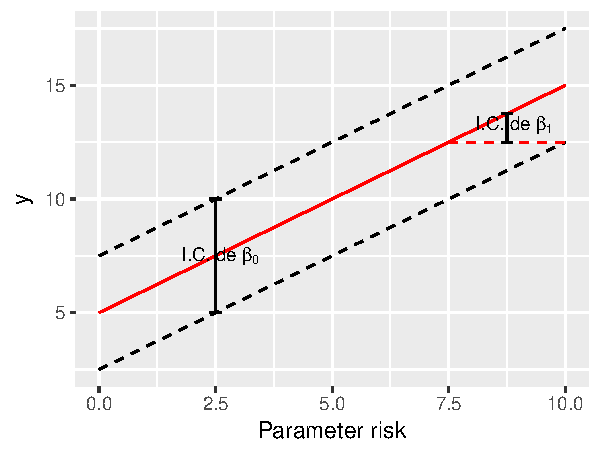
\includegraphics{notes_de_cours-017}

Étant donné que $|-3.040| < -1.78$, on rejette $H_0$ au niveau de confiance de 95 \%. Autrement dit, la pente de la droite est significativement négative.

\subsubsection*{Question 4}
Obtenir un I.C. au niveau de confiance de 95 \% pour $\beta_0$.

\begin{align*}
\beta_0 &\in \hat{\beta}_0 \pm t_{\frac{0.05}{2}}(14-2)\sqrt{\widehat{Var}(\hat{\beta}_0)} \\
& \in 68.494 \pm 2.18 \times \sqrt{66.8511} \\
&\in \big] 50.670, 86.318 \big[
\end{align*}
L' I.C. permet de valider le test d'hypothèse de la question 1, car il ne comprend pas la valeur zéro.

\subsubsection*{Question 5}
Obtenir un I.C. au niveau de confiance de 95 \% pour $\beta_1$.

\begin{align*}
\beta_1 &\in \hat{\beta}_1 \pm t_{\frac{0.05}{2}}(14-2)\sqrt{\widehat{Var}(\hat{\beta}_1)} \\
& \in -0.468 \pm 2.18 \times \sqrt{0.0237} \\
&\in \big] -0.804, -0.132 \big[
\end{align*}
L'I.C. permet de valider le test d'hypothèse de la question 2 et 3, il ne comprend pas la valeur zéro et est strictement négatif.

\subsection{Test de la validité \emph{globale} de la régression}
Une régression linéaire simple est valide, ou significative si $\beta_1 \neq 0$. Le tableau ANOVA obtenue en \ref{seq:anova} peut être utilisé pour tester les hypothèses :
\begin{align*}
H_0 &: \beta_1 = 0\\
H_1 &: \beta_1 < 0 \\
&\text{avec la statistique de Fisher, } \\
F &= \frac{MSR}{MSE} \\
&= \frac{\frac{SSR}{1}}{\frac{SSE}{(n-2)}} \\
\end{align*}
Sous $H_0$, on a que $F \sim F(1, n-2)$. \\
On rejette donc $H_0$ au niveau $100 \times (1 - \alpha) \%$ si
\begin{equation}
\label{eq:fisher}
\color{blue}
\boxed{\color{black}
F > F_{\alpha}(1, n-2)}
\end{equation}

\begin{moreInfo}{\emph{Équivalent}}
\label{equivalent}
	En régression linéaire simple \textbf{seulement}, le test F est équivalent au test $t$ pour $\beta_1 = 0$
	\begin{align*}
	F &= \frac{\frac{SSR}{1}}{\frac{SSE}{(n-2)}} = \frac{SSR}{\sigma^2} = \frac{SSR}{S^2} = \frac{\sum_{t=1}^n (\hat{Y}_t - \overline{Y})^2}{S^2} \\
	&= \frac{\sum_{t=1}^n(\hat{\beta}_0 + \hat{\beta}_1X_t - \hat{\beta}_0 - \hat{\beta}_1\overline{X})^2}{S^2} = \frac{\hat{\beta}_1^2 \times \sum_{t=1}^n(X_t - \overline{X})^2}{S^2} \\
	&= \frac{\hat{\beta}_1^2}{\frac{S^2}{\sum_{t=1}^n(X_t - \overline{X})^2}} \\
	&= \frac{(\hat{\beta}_1 - 0)^2}{\widehat{Var}(\hat{\beta}_1)} \\
	&= t^2
	\end{align*}
\end{moreInfo}

\bigskip
On poursuit avec un exemple pour assimiler l'information.

\subsubsection*{Exemple}
Soit le tableau ANOVA suivant :
\begin{center}
\begin{tabular}{|c|c|c|c|c|}
\hline
Source & $SS$ & $d.l.$ & $MS$ & $F$ \\
\hline
Régression & 48.845 & 1 & 48.845 & 9.249 \\
Erreur & 63.374 & 12 & 5.281 & \\
\hline
Total & 112.219 & 13 & & \\
\hline
\end{tabular}
\end{center}
On cherche a vérifier la validité de la régression à l'aide du test $F$. \newline
On a que $F = 9.249$, par contre $F_{0.05}(1, 12) = 4.75$ \newline
Puisque $F>F_{0.05}(1, 12)$; on rejette $H_0$. La régression est significative au niveau de confiance de 95 \%.

\section{Prévisions et intervalles de confiance}
On peut utiliser la droite de régression pour faire des types de prévisions de $Y^*$ en sachant $X^*$ :
\subsubsection*{Type 1}
Prévision pour la \emph{valeur moyenne} de $Y^*$
$$
E[Y^*] = \beta_0 + \beta_1X^*
$$

\subsubsection*{Type 2}
Prévision pour la \emph{vraie valeur} de $Y^*$
$$
Y^* = \beta_0 + \beta_1X^* + \varepsilon
$$

\subsubsection*{Remarques}
\begin{enumerate}
\item Dans les deux types, la prévision est le point sur la droite de régression
\begin{align*}
\widehat{E}[Y^*] &= \hat{Y}^* \\
\hat{Y}^* &= \hat{\beta}_0 +  \hat{\beta}_1X^*
\end{align*}
\item La prévision est sans biais 
\begin{align*}
E[\hat{\beta}_0 +  \hat{\beta}_1X^*] &= E[\hat{\beta}_0] + E[\hat{\beta}_1]X^* \\
&= \beta_0 +  \beta_1X^*
\end{align*}
\item Il y a deux sources d'erreur dans les prévisions,
\begin{itemize}
\item Parameter risk : Incertitude sur les estimateurs. Autrement dit, la variance des estimateurs des paramètres.

%% Figure parameter risk
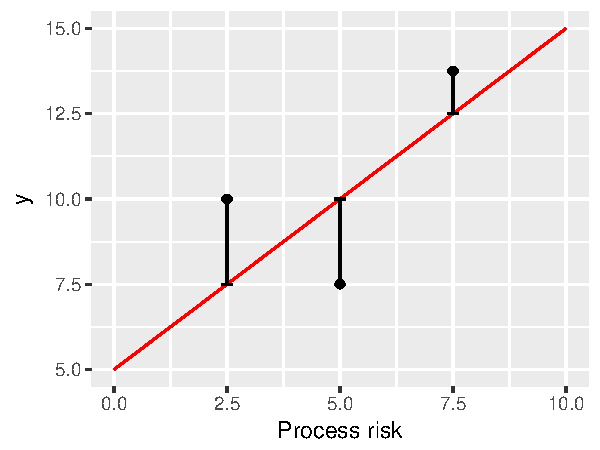
\includegraphics{notes_de_cours-018}
\item Process risk : Fluctuations autour de la droite de régression. Autrement dit, la variance des résidus.

%% Figure process risk
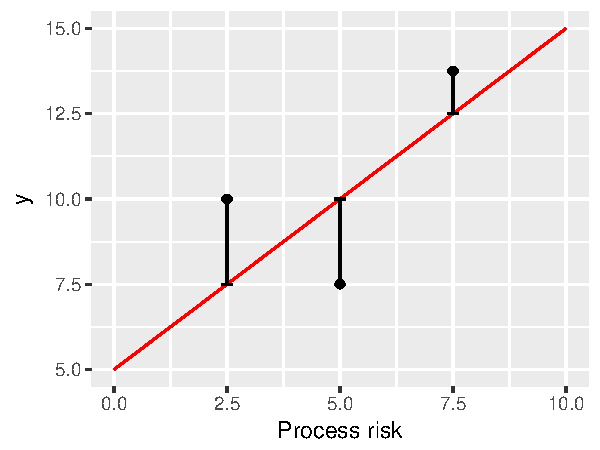
\includegraphics{notes_de_cours-019}
\end{itemize}
\end{enumerate}

Effet combiner des deux sources d'erreur dans les prévisions,

%%Figure combinaison des 2 effets
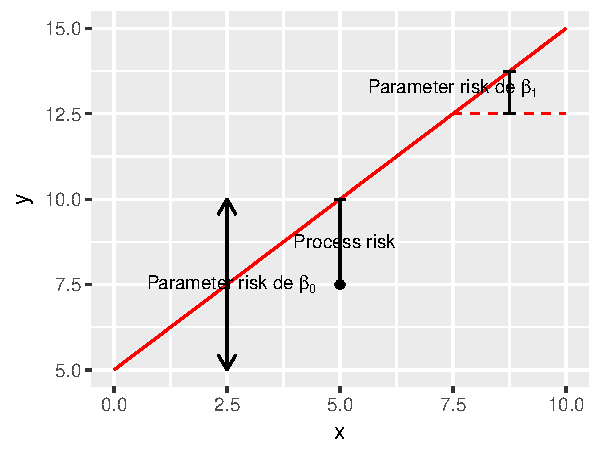
\includegraphics{notes_de_cours-020}

\subsection{I.C. pour la prévision de type I (Valeur moyenne)}
\label{sec:type1}
Aussi appelé intervalle de confiance pour la droite de régression.
\bigskip

Tel que vue à la section \ref{sec:distri}, on a que
$$
\big(\widehat{E}[Y^*] = \hat{\beta}_0 + \hat{\beta}_1X^* \big) \sim N(\beta_0 + \beta_1X^*; Var( \hat{\beta}_0 + \hat{\beta}_1X^*))
$$
Par conséquent,
$$
\frac{(\hat{\beta}_0 + \hat{\beta}_1X^*) - (\beta_0 + \beta_1X^*)}{\sqrt{Var( \hat{\beta}_0 + \hat{\beta}_1X^*)}} \sim N(0,1)
$$
En substituant $\sigma^2$ par $S^2$ dans la $Var(\hat{\beta}_0 + \hat{\beta}_1X^*)$; on a
$$
\frac{(\hat{\beta}_0 + \hat{\beta}_1X^*) - (\beta_0 + \beta_1X^*)}{\sqrt{\widehat{Var}( \hat{\beta}_0 + \hat{\beta}_1X^*)}} \sim t(n-2)
$$
Ainsi, un I.C. au niveau $100 \times(1 -\alpha)\%$ pour la valeur moyenne est

\begin{equation}
\label{eq:IC}
\color{blue}
\boxed{\color{black}
(\hat{\beta}_0 + \hat{\beta}_1X^*)  \pm t_{\frac{\alpha}{2}}(n-2)\times \sqrt{\widehat{Var}( \hat{\beta}_0 + \hat{\beta}_1X^*)}
}
\end{equation}
On rappelle que comme $\sigma^2$ n'est souvent pas connu, il est nécessaire d'utiliser son estimateur $S^2$.

Or, 
\begin{align*}
Var(\hat{\beta}_0 + \hat{\beta}_1X^*)  &= Var(\overline{Y} - \overline{Y} + \hat{\beta}_0 + \hat{\beta}_1X^*) \\
&= Var(\overline{Y} - (\hat{\beta}_0 + \hat{\beta}_1\overline{X}) + \hat{\beta}_0 + \hat{\beta}_1X^*) \\
&= Var(\overline{Y} + \hat{\beta}_1( X^* - \overline{X})) \\
&= Var(\overline{Y}) + Var(\hat{\beta}_1)( X^* - \overline{X})^2 \\
&= \frac{\sigma^2}{n} + \frac{\sigma^2}{\sum_{t=1}^n (X_t - \overline{X})^2}(X^* - \overline{X})^2 \\
&=\sigma^2 \Bigg(\frac{1}{n} + \frac{(X^* - \overline{X})^2 }{\sum_{t=1}^n (X_t - \overline{X})^2}\Bigg)  \\
\end{align*}
Et ainsi, on obtient,

\begin{equation}
\label{eq:var*}
\color{blue}
\boxed{\color{black}
\widehat{Var}(\hat{\beta}_0 + \hat{\beta}_1X^*) = S^2 \Bigg(\frac{1}{n} + \frac{(X^* - \overline{X})^2 }{\sum_{t=1}^n (X_t - \overline{X})^2}\Bigg)  
}
\end{equation}
L'I.C. est donc,
\begin{equation}
\label{eq:IC2}
\color{blue}
\boxed{\color{black}
(\hat{\beta}_0 + \hat{\beta}_1X^*) \pm t_{\frac{\alpha}{2}}(n-2)\times \sqrt{S^2 \bigg(\frac{1}{n} + \frac{(X^* - \overline{X})^2 }{\sum_{t=1}^n (X_t - \overline{X})^2}\bigg)}  
}
\end{equation}

\subsubsection*{Remarque}

%%figure graphique IC
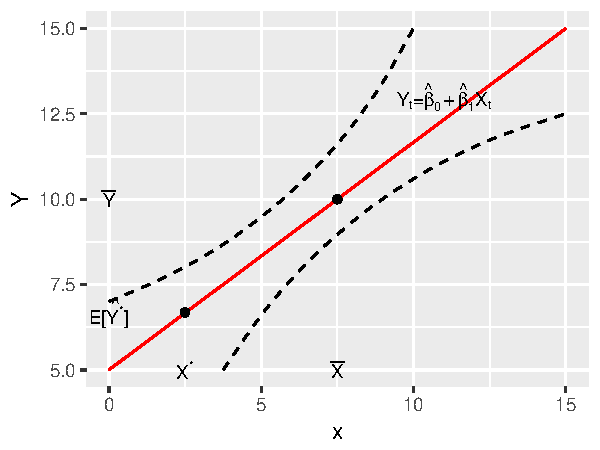
\includegraphics{notes_de_cours-021}

\begin{enumerate}
\item Plus $X^*$ s'éloigne de $\overline{X}$, plus l'I.C. est large, parce que l'incertitude augmente.
\item Les limites de l'intervalle sont des \emph{hyperboles} centrées en $(\overline{X}, \overline{Y})$
\item Cet I.C. peut être appelé :
     \begin{itemize}
     \item I.C. pour la valeur moyenne;
     \item I.C. pour la droite de régression;
     \item I.C. pour la tendance.
     \end{itemize}
\item Dans ce type d' I.C., on tient seulement compte du \textbf{risque de paramètre}.
\end{enumerate}

\subsection{I.C. pour la prévision de type II (Vraie valeur)}
\label{sec:type2}
Aussi appelé I.C. pour les points de $Y^*$.
\bigskip
Pour obtenir un I.C. pour la vraie valeur de $Y^*$, il faut tenir compte du parameter risk $(Var(\hat{\beta}_i))$ ET du process risk $(Var(\varepsilon_t))$. On considère donc de manière équivalente à la section \ref{sec:type1},

$$
\frac{Y^* - \hat{Y}^*}{\sqrt{Var(Y^* - \hat{Y}^*)}} \sim N(0,1)
$$
En substituant $\sigma^2$ par $S^2$ dans $Var(Y^* - \hat{Y}^*)$, on a

$$
\frac{Y^* - \hat{Y}^*}{\sqrt{\widehat{Var}(Y^* - \hat{Y}^*)}} \sim t(n-2)
$$
Ainsi, un I.C. au niveau $100 \times (1 - \alpha)\%$ pour $\beta_1$  pour la vraie valeur de $Y^*$ est,
$$
\hat{Y}^* \pm t_{\frac{\alpha}{2}}(n-2)\times \sqrt{\widehat{Var}(Y^* - \hat{Y}^*)}
$$

Or par hypothèse on a
\begin{align*}
Var(Y^* - \hat{Y}^*) &= Var(Y^*) + Var(\hat{Y}^*) \\
&= \underbrace{\sigma^2} +\underbrace{\sigma^2\big( \frac{1}{n} + \frac{(X^* - \overline{X}^*)^2}{\sum_{t=1}^n (X_t - \overline{X}^*)^2}\big)}  \\
&   \text{Process risk }\ \ \ \  \text{Parameter risk}
\end{align*}
D'où 

\begin{equation}
\label{eq:var2*}
\color{blue}
\boxed{\color{black}
\widehat{Var}(Y^* - \hat{Y}^*) = S^2 \Bigg(1 + \frac{1}{n} + \frac{(X^* - \overline{X}^*)^2}{\sum_{t=1}^n (X_t - \overline{X}^*)^2}\Bigg)  
}
\end{equation}
L'I.C. est donc,
\begin{equation}
\label{eq:IC3}
\color{blue}
\boxed{\color{black}
(\hat{\beta}_0 + \hat{\beta}_1X^*) \pm t_{\frac{\alpha}{2}}(n-2)\times \sqrt{S^2 \Bigg(1 + \frac{1}{n} + \frac{(X^* - \overline{X}^*)^2}{\sum_{t=1}^n (X_t - \overline{X}^*)^2}\Bigg)}  
}
\end{equation}

\subsubsection*{Exemple en R}
Il est possible d'obtenir le résultat des formules des sections \ref{sec:type1} et \ref{sec:type2}.

\subsubsection*{I.C. de type I pour tous les X dans les observations}
\begin{Schunk}
\begin{Soutput}
          fit         lwr       upr
1 -1.04193251 -2.19692700 0.1130620
2  0.53665146 -0.06161401 1.1349169
3  0.36536496 -0.23811573 0.9688456
4  1.15624754  0.42288794 1.8896071
5  0.02261482 -0.64787851 0.6931081
\end{Soutput}
\end{Schunk}

\subsubsection*{I.C. de type I pour un vecteur $X^*$}
\begin{Schunk}
\begin{Soutput}
        fit         lwr       upr
1 0.2717674 -0.34293768 0.8864724
2 0.5556604 -0.04327315 1.1545939
3 0.8395533  0.20220518 1.4769015
4 1.1234463  0.40210294 1.8447896
5 1.4073393  0.57002685 2.2446517
\end{Soutput}
\end{Schunk}

\subsubsection*{I.C. de type II pour un vecteur $X^*$}
\begin{Schunk}
\begin{Soutput}
        fit       lwr      upr
1 0.2717674 -2.123241 2.666776
2 0.5556604 -1.835349 2.946669
3 0.8395533 -1.561366 3.240473
4 1.1234463 -1.301124 3.548016
5 1.4073393 -1.054224 3.868903
\end{Soutput}
\end{Schunk}

\begin{lstlisting}[linerange=\\begin\{Sinput\}-\\end\{Sinput\},includerangemarker=false, caption = Code source en R pour l'exemple]
\begin{Schunk}
\begin{Sinput}
> # dataset
> x <- rnorm(15)
> y <- x + rnorm(15)
> xStar <- data.frame(x = seq(0, 2, by = 0.2)) 
> # Modele de regression
> fit <- lm(y ~x)
> # I.C. de type 1
> predict(fit, interval = "confidence") # I.C. pour tous les X dans les observations
> predict(fit, interval = "confidence", newdata = xStar) # I.C. pour un vecteur de X^*
> # I.C. de type 2
> predict(fit, interval = "prediction", newdata = xStar) # I.C. pour un vecteur de x^*
\end{Sinput}
\end{Schunk}
\end{lstlisting}
\bigskip

\chapter{Régression multiple}
Il n'est pas rare que plus d'une variable soit nécessaire pour expliquer un phénomène. 
Tel que vue à la section \ref{ex:multiple}, voici un exemple de modèle de régression multiple :

\bigskip

%%% fig linéaire multiples
\begin{center}
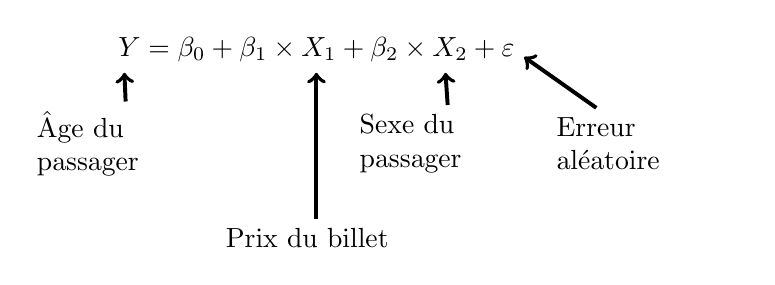
\begin{tikzpicture}[node distance=1.2cm]
\node (function) at (current page.center) {$Y  = \beta_0 + \beta_1 \times X_1 + \beta_2 \times X_2 + \varepsilon$};
\coordinate[below of=function] (c);
\node[text width = 2.3cm, left of=c, xshift=-1.2cm]  (Y) {Âge du passager};
\draw[->, line width=0.5mm] (Y) -- ([xshift=2mm, yshift=-3mm] function.west);
\node[text width = 2.3cm, below of=c, yshift=-0.0001cm] (X) {Prix du billet};
\draw[->, line width=0.5mm] (X) -- ([xshift=0cm, yshift=-3mm] function.center);
\node[text width = 2.3cm, right of=c, xshift=0.5cm] (X2) {Sexe du passager};
\draw[->, line width=0.5mm] (X2) -- ([xshift=-1cm, yshift=-3mm] function.east);
\node[text width = 2.3cm, right of=c, xshift=3cm] (E) {Erreur aléatoire};
\draw[->, line width=0.5mm] (E) -- ([ yshift=-1mm] function.east);
\end{tikzpicture}
\end{center}

De manière générale, la régression multiple considère le modèle général suivant :
\begin{align*}
Y_t &= \beta_0 + \beta_1X_{t,1} + \beta_2X_{t,2} + ... + \beta_pX_{t,p} + \varepsilon_t \text{ , pour } t = 1,...,n \\
& \bullet \text{ n observations} \\
& \bullet \text{ p variables exogènes }(X_1,...,X_p)\\
& \bullet (p+1) \text{ paramètres à estimer} (\beta_0,\beta_1,...,\beta_p)
\end{align*}

\section*{Quelques éléments d'algèbre matricielle pour les vecteurs et matrices aléatoires}
Soient $X_1,...X_n$ des variables aléatoires, on définit le vecteur aléatoire X suivant
\begin{align*}
\mathbb{X} &=
\begin{bmatrix} 
X_1 \\
X_2 \\
\vdots \\
X_n \\
\end{bmatrix}_{n \times 1}
\end{align*}

On définit le vecteur espérance de la façon suivante
\begin{align*}
E[X] &=
\begin{bmatrix} 
E[X_1] \\
E[X_2 ]\\
\vdots \\
E[X_n] \\
\end{bmatrix}_{n \times 1}
\end{align*}

et la matrice de variance-covariance
\begin{align*}
Var(X) &=\underbrace{E\Big[(X -E[X])(X-E[X])^\intercal\Big]}  =
\begin{bmatrix} 
Var(X_1) &\cdots & Cov(X_1,X_n) \\
\vdots \\
Cov(X_n,X_1) & \cdots & Var(X_n)\\
\end{bmatrix}_{n \times 1}\\
& \text{\ \ \ \ \ \ Produit matriciel}
\end{align*}

\subsubsection*{Théorème}
\label{sec:theo}

Soit $\mathbb{X}$, un vecteur aléatoire et $\mathbb{A}$ une matrice de constantes telle que :
$$
\mathbb{X} = \mathbb{X}_{n \times 1} \text{ et } \mathbb{A} = \mathbb{A}_{p \times n}
$$
Alors,
\begin{align*}
E[\mathbb{AX}] &= \mathbb{A}E[\mathbb{X}] \\
Var(\mathbb{A}\mathbb{X}) &= \mathbb{A} Var(\mathbb{X})\mathbb{A}^\intercal \\
\end{align*}

\subsubsection*{Exemple}
\begin{align*}
\mathbb{A} &= 
     \begin{bmatrix} 
     1 \\
     1\\
     \end{bmatrix}_{2 \times 1}^\intercal 
  = \begin{bmatrix} 
     1 & 1 \\
     \end{bmatrix}_{1 \times 2} \\
\mathbb{X} &= 
     \begin{bmatrix} 
     X_1 \\
     X_2\\
     \end{bmatrix}_{2 \times 1}\\
\end{align*}

Intuitivement,
\begin{align*}
\mathbb{A} \mathbb{X} &= X_1 + X_2  \\
\Rightarrow & E[\mathbb{A} \mathbb{X}] = E[X_1 + X_2] = E[X_1] + E[X_2] \\
\Rightarrow & Var(\mathbb{A} \mathbb{X})= Var(X_1 + X_2) = Var(X_1) + Var(X_2) + 2cov(X_1, X_2) \\
\end{align*}

En calcul matriciel,
\begin{align*}
E[\mathbb{A} \mathbb{X}] &= \mathbb{A} E[\mathbb{X}]  \\
&= 
\begin{bmatrix} 
     1 & 1 \\
\end{bmatrix} 
\begin{bmatrix} 
     E[X_1] \\
     E[X_2]\\
\end{bmatrix} \\
&= E[X_1] + E[X_2] \\
Var(\mathbb{A} \mathbb{X}) &= \mathbb{A}Var(\mathbb{X})\mathbb{A}^\intercal \\
&= 
\begin{bmatrix} 
     1 & 1 \\
\end{bmatrix}
\begin{bmatrix} 
Var(X_1)  & Cov(X_1,X_2) \\
Cov(X_1,X_2) & Var(X_2)\\
\end{bmatrix} 
\begin{bmatrix} 
     1  \\
     1  \\
\end{bmatrix}\\
&= 
\begin{bmatrix} 
\big(Var(X_1)  + Cov(X_1,X_2) \big) &\big(Cov(X_1,X_2) + Var(X_2) \big) 
\end{bmatrix}
\begin{bmatrix} 
     1  \\
     1  \\
\end{bmatrix}\\
&= Var(X_1) + Var(X_2) + 2cov(X_1, X_2) \\
\end{align*}

\section{Le modèle sous forme matricielle}
À partir du modèle général suivant, 
\begin{align*}
Y_t &= \beta_0 + \beta_1X_{t,1} + \beta_2X_{t,2} + ... + \beta_pX_{t,p} + \varepsilon_t, t = 1,...,n \\
\end{align*}
On représente les n formules suivantes
\begin{align*}
Y_1 &= \beta_0 + \beta_1X_{1,1} + ... + \beta_pX_{1,p} + \varepsilon_1 \\
Y_2 &= \beta_0 + \beta_1X_{2,1} + ... + \beta_pX_{2,p} + \varepsilon_2 \\
\vdots& \\
Y_n &= \beta_0 + \beta_1X_{n,1} + ... + \beta_pX_{n,p} + \varepsilon_n \\
\end{align*}
Qu'il est possible de réécrire sous forme matricielle,
\begin{align*}
\begin{bmatrix} 
Y_1  \\
Y_2  \\
\vdots \\
Y_n \\
\end{bmatrix}_{n\times 1} =
\begin{bmatrix} 
\beta_0 + \beta_1X_{1,1} + ... + \beta_pX_{1,p} \\
\beta_0 + \beta_1X_{2,1} + ... + \beta_pX_{2,p}  \\
\vdots \\
\beta_0 + \beta_1X_{n,1} + ... + \beta_pX_{n,p} \\
\end{bmatrix}_{n\times 1} + 
\begin{bmatrix} 
\varepsilon_1 \\
\varepsilon_2 \\
\vdots \\
\varepsilon_n \\
\end{bmatrix}_{n\times 1} 
\end{align*}

Ou encore de la façon suivante,

\begin{align*}
\begin{bmatrix} 
Y_1  \\
Y_2  \\
\vdots \\
Y_n \\
\end{bmatrix}_{n\times 1} =
\begin{bmatrix} 
1 & X_{1,1} & ... & X_{1,p} \\
1 & X_{2,1} & ... & X_{2,p}  \\
\vdots & \vdots & \vdots & \vdots \\
1 &  X_{n,1} & ... & X_{n,p} \\
\end{bmatrix}_{n\times (p + 1)} 
\begin{bmatrix} 
\beta_1 \\
\beta_2  \\
\vdots \\
\beta_p \\
\end{bmatrix}_{(p + 1) \times 1}+ 
\begin{bmatrix} 
\varepsilon_1 \\
\varepsilon_2 \\
\vdots \\
\varepsilon_n \\
\end{bmatrix}_{n\times 1} 
\end{align*}

De manière plus compacte, on utilise la notation suivante
$$
\mathbb{Y} = \mathbb{X}  \mathbb{\beta}  + \mathbb{\varepsilon}  
$$
, avec :
\begin{itemize}
\item $Y$ est un vecteur de de dimension $n \times 1$ des variables réponses.
\item $X$ est une matrice schéma de dimension $n \times (p+1)$ qui correspond au variables explicatives.
\item $\beta$ est un vecteur de dimension $(p+1) \times 1$ des coefficients à estimer.
\item $\varepsilon$ est un vecteur de dimension $n \times 1$ des erreurs de telle sorte que
     \begin{itemize}
     \item $E[\varepsilon] = \mathbb{O}_{n\times 1}$, où $\mathbb{O}$ correspond à une matrice nulle.
     \item $Var(\varepsilon) = \sigma^2 \mathbb{I}_{n \times n}$, où $\mathbb{I}$ correspond à une matrice identité.
     \end{itemize}
\end{itemize}

\subsubsection*{Remarques}
\begin{enumerate}
\item \label{remarque1} On suppose que $(\mathbb{X}^\intercal \mathbb{X})^{-1}$ existe, que $\mathbb{X}$ est de rang complet et que $\bigg((\mathbb{X}^\intercal \mathbb{X})^{-1}\bigg)^\intercal = (\mathbb{X}^\intercal \mathbb{X})^{-1}$
\item Pour un modèle de régression linéaire simple, il suffit de définir la matrice schéma de la façon suivante:
$$
\mathbb{X} = 
\begin{bmatrix} 
1 & X_{1} \\
1 & X_{2} \\
\vdots & \vdots  \\
1 &  X_{n} \\
\end{bmatrix}_{n\times 2} 
$$
\item Pour un modèle passant par l'origine, il n'y a pas de colonne de \emph{1} dans la matrice schéma :
\begin{align*}
\mathbb{X} = 
\begin{bmatrix} 
X_{1,1} & ... & X_{1,p} \\
X_{2,1} & ... & X_{2,p}  \\
\vdots & \vdots & \vdots \\
X_{n,1} & ... & X_{n,p} \\
\end{bmatrix}_{n\times (p)} 
\end{align*}
\item Pour un modèle du type $ Y_t = \beta_0 + \beta_1X_{t} + \beta_2X_{t}^2 + \varepsilon_t $, il ne suffit que de définir la matrice schéma telle que :
\begin{align*}
\mathbb{X} &= 
\begin{bmatrix} 
1 & X_{1} & ... & X_{1}^2 \\
\vdots & \vdots & \vdots & \vdots \\
1 &  X_{n} & ... & X_{n}^2 \\
\end{bmatrix}_{n\times (p)} \\
X_{t,1} &= X_t \\
X_{t,2} &= X_t^2
\end{align*}
\end{enumerate}

\subsection{Estimateur des moindes carrés (EMC)}
On peut démontrer que l'estimateur $\hat{\beta}$ de $\hat{\beta}$ qui minimise la somme résiduelle des carrés correspond à l'équation suviante :
\begin{align*}
S(\beta) &= \sum_{t=1}^n (Y_t - \hat{Y}_t)^2 \\
&= \sum_{t=1}^n \varepsilon_t^2 \\
&= \utilde{\varepsilon}^\intercal \varepsilon \\
&= (\mathbb{Y} - \mathbb{X} \beta)^\intercal(\mathbb{Y} - \mathbb{X}\beta)
\end{align*}
est donné par
\begin{equation}
\label{eq:betamulti}
\color{blue}
\boxed{\color{black}
\hat{\beta} = (\mathbb{X}^\intercal\mathbb{X})^{-1}\mathbb{X}^\intercal\mathbb{Y}}
\end{equation}

\subsubsection*{Exemple}
On poursuit avec un exemple en régression linéaire simple pour assimiler l'information. \newline
À l'aide des matrices suivantes, déterminer les paramètres de la droite de régression.
%% matrice initiale
\begin{align*}
\mathbb{Y} =
\begin{bmatrix} 
Y_{1} \\
\vdots  \\
Y_{n} \\ 
\end{bmatrix}; 
\mathbb{X} =
\begin{bmatrix} 
1 & X_{1} \\
\vdots & \vdots  \\
1 & X_{n} \\ 
\end{bmatrix};
\mathbb{X}^\intercal =
\begin{bmatrix} 
1 & \cdots & 1 \\
X_1  & \cdots & X_{n} \\ 
\end{bmatrix}
\end{align*}

%% X'X
\begin{align*}
\mathbb{X}^\intercal \mathbb{X} &=
\begin{bmatrix} 
1 & \cdots & 1 \\
X_1  & \cdots & X_{n} \\ 
\end{bmatrix}
\begin{bmatrix} 
1 & X_{1} \\
\vdots & \vdots  \\
1 & X_{n} \\ 
\end{bmatrix} \\
&= 
\begin{bmatrix} 
n & \sum_{t=1}^n X_{t} \\
\sum_{t=1}^n X_{t} & \sum_{t=1}^n X_{t}^2 \\ 
\end{bmatrix}
\end{align*}

%% X'X ^-1
\begin{align*}
(\mathbb{X}^\intercal \mathbb{X})^{-1} &=
\frac{1}{n X_{t}^2 - (n \overline{X})^2}
\begin{bmatrix} 
\sum_{t=1}^n X_{t}^2  & n \overline{X} \\
n \overline{X} & n \\ 
\end{bmatrix}
\end{align*}

%% X'Y
\begin{align*}
\mathbb{X}^\intercal \mathbb{Y} &=
\begin{bmatrix} 
1 & \cdots & 1 \\
X_1  & \cdots & X_{n} \\ 
\end{bmatrix} 
\begin{bmatrix} 
Y_{1} \\
\vdots  \\
Y_{n} \\ 
\end{bmatrix} \\
&=
\begin{bmatrix} 
\sum_{t=1}^n Y_{t} \\
\sum_{t=1}^n X_t Y_{t} \\ 
\end{bmatrix} \\
&= 
\begin{bmatrix} 
n \overline{Y} \\
\sum_{t=1}^n X_t Y_{t} \\ 
\end{bmatrix} \\
\end{align*}

Ainsi,
\begin{align*}
\hat{\beta} &= 
\begin{bmatrix} 
\hat{\beta}_0 \\
\hat{\beta}_1 \\
\end{bmatrix} \\
&= (\mathbb{X}^\intercal\mathbb{X})^{-1}\mathbb{X}^\intercal\mathbb{Y} \\
&= 
\begin{bmatrix} 
\frac{n \overline{Y} \sum_{t=1}^n X_t^2 - n \overline{X} \sum_{t=1}^n X_tY_t}{n \sum_{t=1}^n X_t^2 - (n \overline{X})^2} \\
\frac{n\sum_{t=1}^n X_tY_t - (n \overline{Y})(n \overline{X}) }{n \sum_{t=1}^n X_t^2 - (n \overline{X})^2} \\
\end{bmatrix} \\
&=
\begin{bmatrix} 
\frac{\overline{Y} \sum_{t=1}^n X_t^2 - \overline{X} \sum_{t=1}^n X_tY_t + n\overline{X}^2\overline{Y} - n\overline{X}^2\overline{Y}}{n \sum_{t=1}^n X_t^2 - (n \overline{X})^2} \\
\frac{\sum_{t=1}^n X_tY_t - n\overline{Y}\overline{X}}{\sum_{t=1}^n X_t^2 - n \overline{X}^2} \\
\end{bmatrix} \\
&=
\begin{bmatrix} 
\overline{Y} - \hat{\beta}_1\overline{X} \\
\hat{\beta}_1 \\
\end{bmatrix} \\
\end{align*}
Qui corresponde bien aux estimateurs de $\hat{\beta}_0$ (\ref{eq:beta0}) et $\hat{\beta}_1$ (\ref{eq:beta1}) trouver précédament.

\subsection*{Propriétés des estimateurs}
\begin{enumerate}
\item Sans biais
\begin{align*}
E[\hat{\beta}] &= E\big[ (\mathbb{X}^\intercal\mathbb{X})^{-1}\mathbb{X}^\intercal\mathbb{Y} \big] \\
&\overset{\ref{sec:theo}}{=} (\mathbb{X}^\intercal\mathbb{X})^{-1}\mathbb{X}^\intercal E[\mathbb{Y}] \\
&= (\mathbb{X}^\intercal\mathbb{X})^{-1}\mathbb{X}^\intercal (\mathbb{X}\beta) \\
&= (\mathbb{X}^\intercal\mathbb{X})^{-1}(\mathbb{X}^\intercal\mathbb{X}) \beta \\
&= \mathbb{I} \beta \\
&= \beta \\
\end{align*}
\item Variance-covariance
\begin{align*}
Var\hat{\beta}) &= Var\big((\mathbb{X}^\intercal\mathbb{X})^{-1}\mathbb{X}^\intercal\mathbb{Y} \big) \\
&\overset{\ref{sec:theo}}{=} (\mathbb{X}^\intercal\mathbb{X})^{-1}\mathbb{X}^\intercal Var(\mathbb{Y}) \big[ (\mathbb{X}^\intercal\mathbb{X})^{-1}\mathbb{X}^\intercal \big]^\intercal \\
&= (\mathbb{X}^\intercal\mathbb{X})^{-1}\mathbb{X}^\intercal \sigma^2 \mathbb{I} \bigg[ \mathbb{X} \big[(\mathbb{X}^\intercal\mathbb{X})^{-1} \big]^\intercal \bigg] \\
& \overset{\ref{remarque1}}{=}\sigma^2 (\mathbb{X}^\intercal\mathbb{X})^{-1} \mathbb{X}^\intercal \bigg[ \mathbb{X} \big[(\mathbb{X}^\intercal\mathbb{X})^{-1} \big] \bigg] \\
&= \sigma^2 (\mathbb{X}^\intercal\mathbb{X})^{-1} (\mathbb{X}^\intercal\mathbb{X}) (\mathbb{X}^\intercal\mathbb{X})^{-1} \\
&= \sigma^2 \mathbb{I} (\mathbb{X}^\intercal\mathbb{X})^{-1} \\
&= \sigma^2 (\mathbb{X}^\intercal\mathbb{X})^{-1} \\
\end{align*}
\end{enumerate}

\subsection{Résidus et tableau ANOVA}
On définit les résidus comme ceci,
\begin{align*}
\varepsilon_{n \times 1} &= \mathbb{Y} - \hat{\mathbb{Y}} \\
&= \mathbb{Y} - \mathbb{X} \hat{\beta} \\
&= \mathbb{Y} - \mathbb{X}(\mathbb{X}^\intercal\mathbb{X})^{-1}\mathbb{X}^\intercal\mathbb{Y} \\
&= \mathbb{Y} (\mathbb{I} - \mathbb{X}(\mathbb{X}^\intercal\mathbb{X})^{-1}\mathbb{X}^\intercal) \\
&= \mathbb{Y} (\mathbb{I} - \mathbb{H}) \\
\end{align*}
Où $\mathbb{H}$ correspond à la matrice de projection (Hat matrix).\newline

Les sommes des carrés du tableau ANOVA sont données par les expressions suivantes :

\begin{align*}
\bullet SST &= \sum_{t=1}^n(Y_t - \overline{Y})^2 \\
&= \sum_{t=1}^nY_t^2 - n\overline{Y}^2 \\
&= \mathbb{Y}^\intercal\mathbb{Y} - n \overline{Y}^2 \\
& \text{Avec $(n-1)$ degré de liberté} \\
\end{align*}
\begin{align*}
\bullet SSE &= \sum_{t=1}^n(Y_t - \hat{Y})^2 \\
&= \sum_{t=1}^n\varepsilon_t^2 \\
&= \mathbb{\varepsilon}^\intercal\mathbb{\varepsilon}\\
& \text{Avec $(n-(p+1))$ degré de liberté} \\
\bullet SSR &= \sum_{t=1}^n(\hat{Y_t} - \hat{Y})^2 \\
&= \sum_{t=1}^n\hat{Y_t}^2 - n\overline{Y}^2 \\
&= \mathbb{\hat{Y}}^\intercal\mathbb{\hat{Y}} - n \overline{Y}^2\\
& \text{Avec $(p)$ degré de liberté}
\end{align*}

\bigskip
Dans le cas de régression multiple, le tableau ANOVA est le suivant :

\bigskip
\begin{tabularx}{\linewidth}{|X|X|X|X|X|}
\hline
Source de la variance & Somme des carrés $(SS)$ & Degrés de liberté $(d.l.)$ & Carrés moyens $(MS)$ & Ratio de Fisher $(F)$ \\
\hline
Régression & $SSR$ & p & $\frac{SSR}{p}$ & $\frac{MSR}{MSE}$ \\
Erreur & $SSE$ & n - (p+1) & $ \frac{SSE}{n-(p+1)}$ & \\
\hline
Total & $SST$ & n - 1 & & \\
\hline
\end{tabularx}

\subsection{Estimateur de $\sigma^2$}
Dans le cas de la régression multiple, on peut démontrer qu'un bon estimateur sans biaais de $\sigma^2$ est $S^2$ sous la forme suivante :
\begin{align*}
S^2 &= MSE \\
&= \frac{SSE}{n -(p+1)}
\end{align*}

\subsection{Intervalles de confiance et tests d'hypothèses}
Essentiellement, on a la même chose qu'au chapitre \ref{chap:2} pour les tests $t$ et $F$, sauf qu'il faut adapter les degrés de liberté. \newline
On rappel qu'avec le postulat 4 (\ref{post4}), on suppose que les résidus suivent une loi normale d'espérance nulle et de variance de $\sigma^2$.
\begin{align*}
\varepsilon_t &\overset{i.i.d.}{\sim} N(0, \sigma^2) \\
\utilde{\varepsilon}_{n \times 1} &\sim N(\mathbb{O}, \sigma^2\mathbb{I}_{n\times n}) \\
\end{align*}
Ainsi on a que $ (\mathbb{Y} = \mathbb{X}  \mathbb{\beta}  + \mathbb{\varepsilon}) \sim N_n(\mathbb{X}\mathbb{\beta}; \sigma^2 \mathbb{I}_{n\times n})$ \newline
et que $\hat{\beta} \sim N_n(\mathbb{\beta}; (\mathbb{X}^\intercal\mathbb{X})^{-1}\sigma^2)$.

\subsection{Test de Student sur un seul paramètre}
On effectue le test suivant, 
\begin{align*}
H_0 &: \beta_i = \beta_i^* \\
H_1 &: \beta_i \neq \beta_i^* \\
&\text{Où $\beta_i^*$ est une constante.} \\
&\text{On teste l'hypothèse à l'aide de la statistique suivante, } \\
t &= \frac{\hat{\beta}_i - \beta_i^* }{\sqrt{[{Var}(\hat{\beta})]_{i+1 \times i+1}}} \sim N(0, 1) \\
&\text{et en remplacant $\sigma^2$ par $S^2$ dans la matrice de la variance, on obtient }\\
t &= \frac{\hat{\beta}_i - \beta_i^* }{\sqrt{[\widehat{Var}(\hat{\beta})]_{i+1 \times i+1}}} \sim t(n-(p+1)) \\
\end{align*}
On rejette $H_0$ au niveau de confiance $100 \times (1 - \alpha)\%$ pour si :
$$
|t| > t_{\frac{\alpha}{2}(n-(p+1))}
$$
Or, on a que $Var(\hat{\mathbb(\beta)}) = (\mathbb{X}^\intercal\mathbb{X})^{-1}\sigma^2$ \newline
Ainsi
\begin{equation}
\label{eq:varmulti}
\color{blue}
\boxed{\color{black}
\widehat{Var}(\hat{\mathbb(\beta)}) = (\mathbb{X}^\intercal\mathbb{X})^{-1}S^2}
\end{equation}

Avec un peu d'algèbre, on transforme ce test d'hypothèse en un intervalle de confiance pour $\beta_i$. L'I.C. marginal est donc le suivant :
\begin{equation}
\label{eq:ICmulti}
\color{blue}
\boxed{\color{black}
\hat{\beta}_i \pm t_{\frac{\alpha}{n}}(n - (p+1)) \times \sqrt{[(\mathbb{X}^\intercal\mathbb{X})^{-1}S^2]}_{i+1 \times i+1} }
\end{equation}

\subsection{Test de Fisher pour la validité globale de la régression}
\label{sec:fisherT}
Dans le cas de la régression multiple, on teste 
\begin{align*}
H_0 &: \beta_1 = \beta_2 = ... = \beta_p = 0 \\
H_1 &: \text{Au moins un coefficient parmi $\beta_1,...,\beta_p$ est $\neq 0$.} \\
&\text{On teste l'hypothèse à l'aide de la statistique suivante, } \\
F &= \frac{MSR}{MSE} \sim F(\text{d.l. de SSR, d.l. de SSE}) \\
F &= \frac{MSR}{MSE} \sim F(p, n - (p+1)) \\
\end{align*}
On rejette $H_0$ au niveau de confiance $100 \times (1 - \alpha)\%$ pour si :
$$
F > F_{\alpha}(p, n-(p+1))
$$

\subsubsection*{Remarque importante}
De manière générale, avec p variables explicatives, on a que :
$$
F \neq t^2
$$
L'égalité ne survient que lorsque $p=1$ (Voir la section \ref{equivalent}).

\subsection{Test de Fisher partiel}
\label{sec:testFpartiel}
À la section \ref{sec:fisherT} on a testé si \textbf{tous les} $\beta_1, \beta_2,...,\beta_p$ étaient nuls. \newline

Dans cette section, on teste simultanément si certains $\beta_i$ parmi $\beta_1, \beta_2,...,\beta_p$ sont nuls.

On teste donc :
\begin{align*}
H_0 &: \text{Un modèle \emph{réduit}, noté $M_0$ dont certains $\beta_i =0$ parmi $\beta_1, \beta_2,...,\beta_p$ est acceptable.} \\
H_1 &: \text{On doit utiliser le modèle \emph{complet}, noté $M_1$ avec les $p$ variables.} \\
\end{align*}
On utilise la statistique de Fisher partielle suivante,
\begin{equation}
\label{eq:fisherpartiel}
\color{blue}
\boxed{\color{black}
F^* = \frac{\frac{[SSE(M_0) - SSE(M_1)]}{[d.l.(SSE(M_0)) - d.l.(SSE(M_1))]}}{\frac{SSE(M_1)}{d.l.(SSE(M_1))}}
}
\end{equation}

On rejette $H_0$ au niveau de confiance $100 \times (1 - \alpha)\%$ si :
$$
F^* > F_{\alpha}\Big( d.l.(SSE(M_0)) - d.l.(SSE(M_1)); d.l.(SSE(M_1)) \Big)
$$

\subsubsection*{Remarque}
Si le modèle réduit de $H_0$ ne consiste qu'à $\beta_i =0$, autrement dit un seul paramètre, alors on aura que $F^* = t^2$. Dans ce cas \textbf{seulement}, le test Fisher partiel est équivalent au test de Student.

\subsubsection*{Exemple}
On poursuit avec un exemple pour assimiler l'information. \newline

Soit le modèle de régression multiple suivant :
$$
Y_t = \beta_0 + \beta_1X_{t,1} + \beta_2X_{t,2} + \beta_3X_{t,3} + \beta_4X_{t,4} + \varepsilon_t
$$

On teste donc :
\begin{align*}
H_0 &: \beta_2 = \beta_3 = 0 \\
H_1 &: \beta_2 \neq 0 \text{ et/ou } \beta_3 \neq 0 \\
\end{align*}

Afin d'effectuer le test, on effectue les étapes suivantes :
\begin{itemize}
\item[\textbf{Étape 1}] Obtenir le tableau ANOVA pour le modèle sous le modèle complet $M_0$. Extraire $SSE(M_0)$ et $d.l.(SSE(M_0)) \Rightarrow n - 3$

\item[\textbf{Étape 2}] Obtenir le tableau ANOVA pour le modèle sous le modèle complet $M_1$. Extraire $SSE(M_1)$ et $d.l.(SSE(M_1)) \Rightarrow n - 5$ 

\item[\textbf{Étape 3}] Calculer la valeur de la statistique de Fisher partielle.
$$
F^* = \frac{\frac{[SSE(M_0) - SSE(M_1)]}{[(n-3) - (n-5)]}}{\frac{SSE(M_1)}{(n-5)}}
$$
Puis rejeter $H_0$ au niveau de confiance $100 \times (1 - \alpha)\%$ si :
$$
F^* > F_{\alpha}\Big( 2; n-5 \Big)
$$
\end{itemize}

\section{Sélection d'un modèle optimal}
\label{sec:optimal}
Lorsque l'on dispose de plusieurs variables explicatives $(X_1,X_2,...,X_p)$, un modèle optimal est tel que :
\begin{enumerate}
\item Pouvoir prédictif \textbf{maximal}
\item Avec un nombre de variables \textbf{minimal}
\end{enumerate}
En régression, il existe plusieurs algorithmes pou obtenir un modèle optimal.

\subsection{Technique 1: Essai de tous les modèles}
\label{tech1}

La stratégie la plus simple consiste à examiner tous les modèles possibles, soit les $2^p$ combinaisons existantes. \newline

On choisi le modèle ayant le plus grand $R^2_{adj}$, qui correspond à l'une des expresions suivantes :

\begin{equation}
\color{blue}
\boxed{\color{black}
R^2_{adj} = 1 - \frac{\frac{SSE}{(n-p-1)}}{\frac{SST}{(n-1)}} 
}
\end{equation}
\begin{equation}
\color{blue}
\boxed{\color{black}
R^2_{adj} = 1 - (1 - R^2) \Big(\frac{n-1}{n-p-1} \Big) 
}
\end{equation}

On note que contrairement au $R^2$, le $R^2_{adj}$ pénalise pour l'ajout de variables dans le modèle.

\bigskip
\subsubsection*{Exemple}
Si on dispose de $X_1, X_2$ et $X_3$, on ajuste les $2^3$ modèles possibles :
\begin{enumerate}
\item $Y = \beta_0 + \varepsilon$
\item $Y = \beta_0 + \beta_1X_1 + \varepsilon$
\item $Y = \beta_0 + \beta_1X_2 + \varepsilon$
\item $Y = \beta_0 + \beta_1X_3 + \varepsilon$
\item $Y = \beta_0 + \beta_1X_1 + \beta_2X_2 + \varepsilon$
\item $Y = \beta_0 + \beta_1X_1 + \beta_2X_3 + \varepsilon$
\item $Y = \beta_0 + \beta_1X_2 + \beta_2X_3 + \varepsilon$
\item $Y = \beta_0 + \beta_1X_1 + \beta_2X_2 + \beta_3X_3 + \varepsilon$
\end{enumerate}
On fait le calcul du $R^2_{adj}$ pour chaque modèle et on choisit le modèle avec le plus grand $R^2_{adj}$.

\subsubsection*{Remarque}
En pratique cette méthode n'est pas \emph{efficiente}, car le temps d'exécution devient énorme lorsque p augmente :

\begin{center}
\begin{tabular}{|c|c|}
\hline
p & $2^p$ \\
\hline
1 & 2 \\
2 & 4 \\
3 & 8 \\
\vdots & \\
10 & 1024 \\
\vdots & \\
25 & 33554432 \\
\vdots & \\
100 & $1.26\times 10^{30}$ \\
\hline
\end{tabular}
\end{center}

\subsection{Technique 2 : Élimination régressive (\emph{Backward elimination})}
\label{tech2}

\begin{itemize}
\item [Étape 1] Débuter avec toutes les variables disponibles dans le modèle.

\item [Étape 2] Chercher la variable qui génère la plus faible augmentation de SSE lorsqu'exclue du modèle. Autrement dit, la pire variable.

\item [Étape 3] Utiliser les test Fisher partiels (\ref{sec:testFpartiel}) pour tester s'il est possible d'exclure la variable de l'étape 2.

\item [Étape 4] Continuer les étapes 2 et 3 jusqu'à ce qu'il n'y ait plus de variables à éliminer selon les tests Fisher partiels.
\end{itemize}
\bigskip

Voici une illustrations de l'élimination régressive.

%% Figure élimination régressive
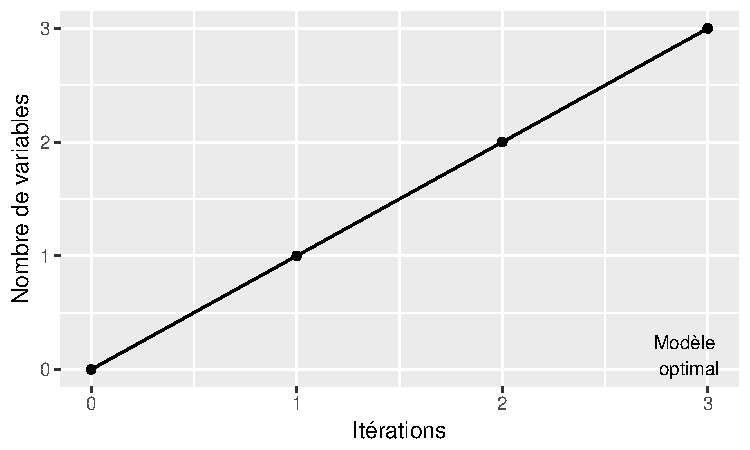
\includegraphics{notes_de_cours-026}

\subsubsection*{Remarque}
Le principal inconvénient de cette technique est qu'une variable éliminée ne peut jamais être réintégrée. 

\subsection{Technique 3 : Sélection progressive (\emph{forward selection})}
\label{tech3}

\begin{itemize}
\item [Étape 1] Débuter avec le modèle $Y = \beta_0 + \varepsilon$

\item [Étape 2] Chercher la variable qui génère la plus grande diminution de SSE lorsqu'incluse dans le modèle. Autrement dit, la meilleure variable.

\item [Étape 3] Utiliser les test Fisher partiels (\ref{sec:testFpartiel}) pour tester s'il est possible d'inclure la variable de l'étape 2.

\item [Étape 4] Continuer les étapes 2 et 3 jusqu'à ce qu'il n'y ait plus de variables à inclures selon les tests Fisher partiels.
\end{itemize}
\bigskip

%% Figure forward technique
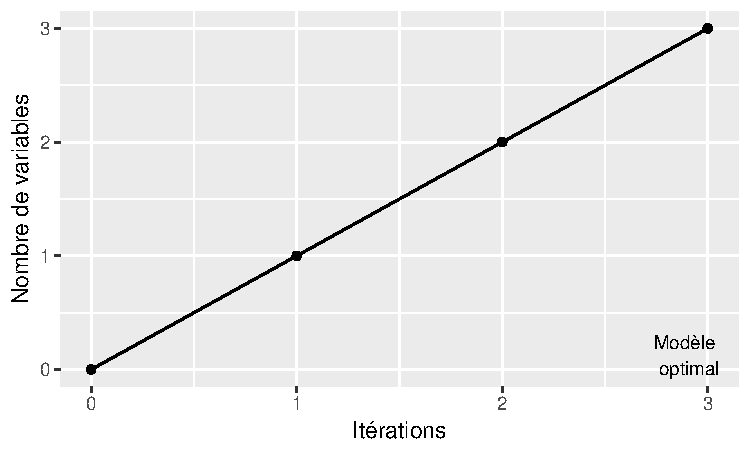
\includegraphics{notes_de_cours-027}

\subsubsection*{Remarque}
Le principal inconvénient de cette technique est qu'une variable incluse ne peut jamais être éliminée par la suite. 

\subsection{Technique 4 : Régression pas à pas (\emph{stepwise regression})}
\label{tech4}

Il s'agit d'une combinaison de l'élimination régressive et de la sélection progressive.

\begin{itemize}
\item [Étape 1] Débuter avec le modèle $Y = \beta_0 + \varepsilon$

\item [Étape 2] Chercher la variable qui génère la plus grande diminution de SSE si incluse dans le modèle. Autrement dit, la meilleure variable.

\item [Étape 3] Utiliser les test Fisher partiels (\ref{sec:testFpartiel}) pour tester s'il est possible d'inclure la variable de l'étape 2.

\item [Étape 4] Chercher la variable qui génère la plus faible diminution de SSE si incluse dans le modèle. Autrement dit, la pire variable.

\item [Étape 5] Utiliser les test Fisher partiels (\ref{sec:testFpartiel}) pour tester s'il est possible d'exclure la variable de l'étape 4.

\item [Étape 6] Continuer les étapes 2 à 5 jusqu'à ce que l'algorithme élimine la variable qui vient d'entrer.
\end{itemize}
\bigskip

%% Figure forward technique
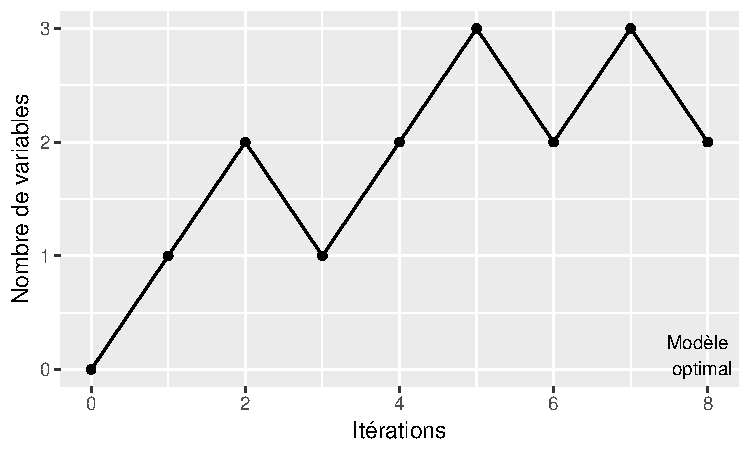
\includegraphics{notes_de_cours-028}

\bigskip
\subsubsection*{Exemple}
On poursuit avec un exemple pour assimiler l'information. \newline
À partir des informations suivantes on cherche à trouver le meilleur modèle de régression des 20 observations.
\bigskip

\begin{tabularx}{\linewidth}{|X|c|c|c|c|}
\hline
Variables dans le modèle & $SSE$ & $SSR$ & $SST$ & $R^2_{adj}$ \\
\hline
$\phi$ & 10 & 0 & 10 & 0 \% \\
$X_1$ & 5 & 5 & 10 & 47.2 \% \\
$X_2$ & 9 & 1 & 10 & 5 \% \\
$X_3$ & 8 & 2 & 10 & 15.5 \% \\
$X_1, X_2$ & 4 & 6 & 10 & 55.3 \% \\
$X_1, X_3$ & 3.9 & 6.1 & 10 & 56.4 \% \\
$X_2, X_3$ & 8.5 & 1.5 & 10 & 5 \% \\
$X_1, X_2, X_3$ & 3.8 & 6.2 & 10 & 54.9 \% \\
\hline
\end{tabularx}

\subsubsection*{Technique 1}
Avec la technique 1 (\ref{tech1}), on trouve le modèle suivant :
$$
Y = \beta_0 + \beta_1X_1 + \beta_2X_2 + \varepsilon
$$

\subsubsection*{Technique 2}
Avec la technique 2 (\ref{tech2}), on débute avec le modèle initial suivant :
$$
Y = \beta_0 + \beta_1X_1 + \beta_2X_2 + + \beta_3X_3 + \varepsilon
$$
La pire variable est $X_2$, on effectue le test de Fisher partiel (\ref{eq:fisherpartiel}) avec modèle $M_0$ sans la variable $X_2$ et $M_1$ avec le modèle complet. 

\begin{align*}
H_0 &: \text{ Modèle avec $X_1$ et $X_3$} \\
H_1 &: \text{ Modèle avec $X_1$, $X_2$ et $X_3$} \\
\end{align*}
\begin{align*}
F &= \frac{\frac{3.9-3.8}{1}}{\frac{3.8}{16}} \\
&= 0.4211 \\
F_{5 \%}(1.16) &= 4.49 \\
0.4211 &< 4.49
\end{align*}
On accepte $H_0$ et on exclut $X_2$. \newline
La prochaine pire variable est la variable $X_1$.

\begin{align*}
H_0 &: \text{ Modèle avec $X_3$} \\
H_1 &: \text{ Modèle avec $X_1$ et $X_3$} \\
\end{align*}
\begin{align*}
F &= \frac{\frac{5 - 3.9}{1}}{\frac{3.9}{17}} \\
&= 4.79 \\
F_{5 \%}(1.17) &= 4.49 \\
4.79 &> 4.45
\end{align*}
On rejette $H_0$ et on n'exclut pas $X_3$. \newline
On trouve le modèle suivant :
$$
Y = \beta_0 + \beta_1X_1 + \beta_2X_3 + \varepsilon
$$

\subsubsection*{Exemple en R}
À l'aide du jeu de donnée \emph{mtcars}\footnote{Voici les \href{https://stat.ethz.ch/R-manual/R-devel/library/datasets/html/mtcars.html}{informations} sur les données.} de \emph{R}, construise un modèle pour prédire la consomation en gallon par miles à l'aide de la technique de régression pas à pas. 
\begin{Schunk}
\begin{Soutput}
Start:  AIC=65.47
mpg ~ wt + drat + disp + qsec + hp

       Df Sum of Sq    RSS    AIC
- disp  1     3.974 174.10 64.205
<none>              170.13 65.466
- hp    1    11.886 182.01 65.627
- qsec  1    12.708 182.84 65.772
- drat  1    15.506 185.63 66.258
- wt    1    81.394 251.52 75.978

Step:  AIC=64.21
mpg ~ wt + drat + qsec + hp

       Df Sum of Sq    RSS    AIC
- hp    1     9.418 183.52 63.891
- qsec  1     9.578 183.68 63.919
<none>              174.10 64.205
- drat  1    11.956 186.06 64.331
+ disp  1     3.974 170.13 65.466
- wt    1   113.882 287.99 78.310

Step:  AIC=63.89
mpg ~ wt + drat + qsec

       Df Sum of Sq    RSS    AIC
<none>              183.52 63.891
- drat  1    11.942 195.46 63.908
+ hp    1     9.418 174.10 64.205
+ disp  1     1.506 182.02 65.627
- qsec  1    85.720 269.24 74.156
- wt    1   275.686 459.21 91.241

Call:
lm(formula = mpg ~ wt + drat + qsec, data = mtcars)

Coefficients:
(Intercept)           wt         drat         qsec  
    11.3945      -4.3978       1.6561       0.9462  
\end{Soutput}
\end{Schunk}
On remarque que la variable $disp$ et $hp$ n'on pas été retenue dans le modèle.

%% script R
\begin{lstlisting}[linerange=\\begin\{Sinput\}-\\end\{Sinput\},includerangemarker=false, caption = Code source en R pour l'exemple]
\begin{Schunk}
\begin{Sinput}
> step(lm(mpg~wt+drat+disp+qsec+hp,data=mtcars),direction="both")
\end{Sinput}
\end{Schunk}
\end{lstlisting}

\begin{moreInfo}{\emph{Technique de sélection \& \emph{R}}}
	Toutes les techniques présentées à la section \ref{sec:optimal} sont intégrer dans le système de base de \emph{R}. Cette \href{https://cran.r-project.org/web/packages/olsrr/vignettes/variable_selection.html}{vignette} sur la sélection des variables comprends les différentes méthodes ainsi que des exemples utile.
\end{moreInfo}

\section{Régression avec variables indicatrices}
Permettent de traiter des variables explicatives \emph{catégoriques} dans les modèles.
\subsubsection*{Exemples}
\begin{itemize}
\item Couleur des yeux (bleu, brun, vert et autres)
\item Type de véhicule (sport et autres)
\item emploi (ACT, ETUm RTR, GOU et autres)
\end{itemize}

Pour inclure une variable catégorique ayant $r$ valeurs possibles, on doit créér $(r-1)$ variables indicatrices.
\subsubsection*{Exemple}
\begin{itemize}
\item Couleur des yeux : 
\begin{align*}
X_{t,1} &= 1_{\{Couleur_t = Bleu\}} \\
X_{t,2} &= 1_{\{Couleur_t = Brun\}} \\
X_{t,3} &= 1_{\{Couleur_t = Vert\}} \\
\end{align*}
\item Type de véhicule :
\begin{align*}
X_{t,4} &= 1_{\{Type_t = Sport\}} \\
\end{align*}
\item Emploi :
\begin{align*}
X_{t,5} &= 1_{\{Emploi_t = ACT\}} \\
X_{t,6} &= 1_{\{Emploi_t = ETU\}} \\
X_{t,7} &= 1_{\{Emploi_t = RTR\}} \\
X_{t,8} &= 1_{\{Emploi_t = GOU\}} \\
\end{align*}
; où 
\begin{align*}
1_{\{A\}} &= 
\left \lbrace
     \begin{array}{rl}
     1 &, \text{si A vrai} \\
     0 &, \text{sinon}
     \end{array}
     \right.
\end{align*}

\end{itemize}

\subsubsection*{Exemple}
À partir des 5 observations suivantes, définir la matrice des variables réponses et la matrice schéma.

\bigskip
\begin{center}
\begin{tabular}{|c|c|c|c|}
\hline
$Y_t$ & $Couleur_t$ & $Type_t$ & $Emploi_t$ \\
\hline
70 & Bleu & Autres & ETU \\
75 & Brun & Sport & GOU \\
50 & Vert & Autres & Autres \\
55 & Autres & Autres & Autres \\
85 & Brun & Sport & ACT \\
\hline
\end{tabular}
\end{center}
\bigskip

On utilise le modèle de régression multiple à partir du modèle d'indicatrice précédent. On obtient le modèle de régression suivant:

\begin{align*}
Y_t &= \beta_0 + \beta_1X_{t,1} + \beta_2X_{t,2} + \beta_3X_{t,3} 
+ \beta_4X_{t,4} + \beta_5X_{t,5} + \beta_6X_{t,6} + \beta_7X_{t,7} + \beta_8X_{t,8} + \varepsilon_t \\
\mathbb{Y} &= \mathbb{X}\mathbb{\beta} + \mathbb{\varepsilon}
\end{align*}

La matrice des variables réponses correspond à :
\begin{align*}
\mathbb{Y} &= 
\begin{bmatrix}
70 \\
75 \\
50 \\
55 \\
85 \\
\end{bmatrix}
\end{align*}

La matrice schéma correspond à :

\begin{align*}
\mathbb{X}
=
\bordermatrix { 
& &  X_1  & X_2 & X_3 & X_4 & X_5  & X_6 & X_7 & X_8 \cr 
& 1 & 1 & 0 & 0 & 0 & 0 & 1 & 0 & 0 \cr 
& 1 & 0 & 1 & 0 & 1 & 0 & 0 & 0 & 1 \cr 
& 1 & 0 & 0 & 1 & 0 & 0 & 0 & 0 & 0 \cr 
& 1 & 0 & 0 & 0 & 0 & 0 & 0 & 0 & 0 \cr 
& 1 & 0 & 1 & 0 & 1 & 1 & 0 & 0 & 0 \cr 
}
\end{align*}

\section{Analyse qualitative des résidus}
Même si les test $t$ et $F$ sont concluents, le modèle choisi peut ne pas être adéquat. En effet, l'analyse qualitative des résidus est la principale façon de valider un modèle sélectionné. 

\subsubsection*{Distribution \emph{uniforme}}
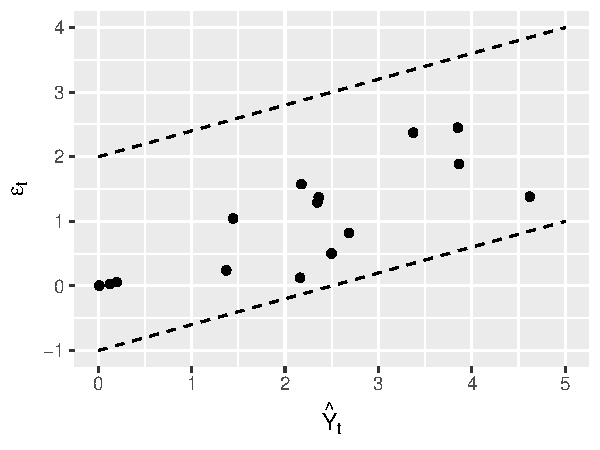
\includegraphics{notes_de_cours-031}

\bigskip
On remarque que les résidus sont uniformément distribués autour de l'axe des $x$. Il s'agit d'une situation idéal.

\subsection{Problèmes possibles dans la distribution des résidus}
Plusieurs problèmes de distribution des résidus peuvent être observés, voici leurs représentations graphiques et leurs possibles significations :

\subsubsection{Distribution \emph{uniforme} avec rotation}
Cette distribution des résidus est très similaire à la distribution \emph{uniforme}, par contre les résidus ne sont pas distribués autour de l'axe des $x$. La distribution semble avoir effectué une rotation. Il manque probalement un terme linéaire dans $X$.

\bigskip
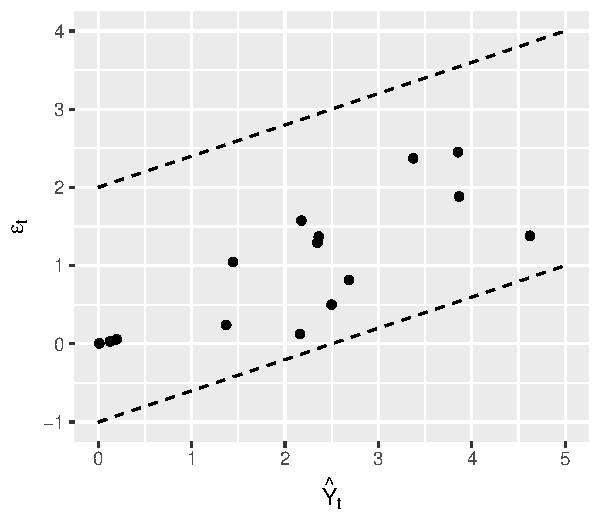
\includegraphics{notes_de_cours-032}
\bigskip

\subsubsection{Distribution \emph{quadratique}}
Cette distribution des résidus semble suivre une distribution quadratique. Il manue probablement une variable quadratique dans $X$.

\bigskip
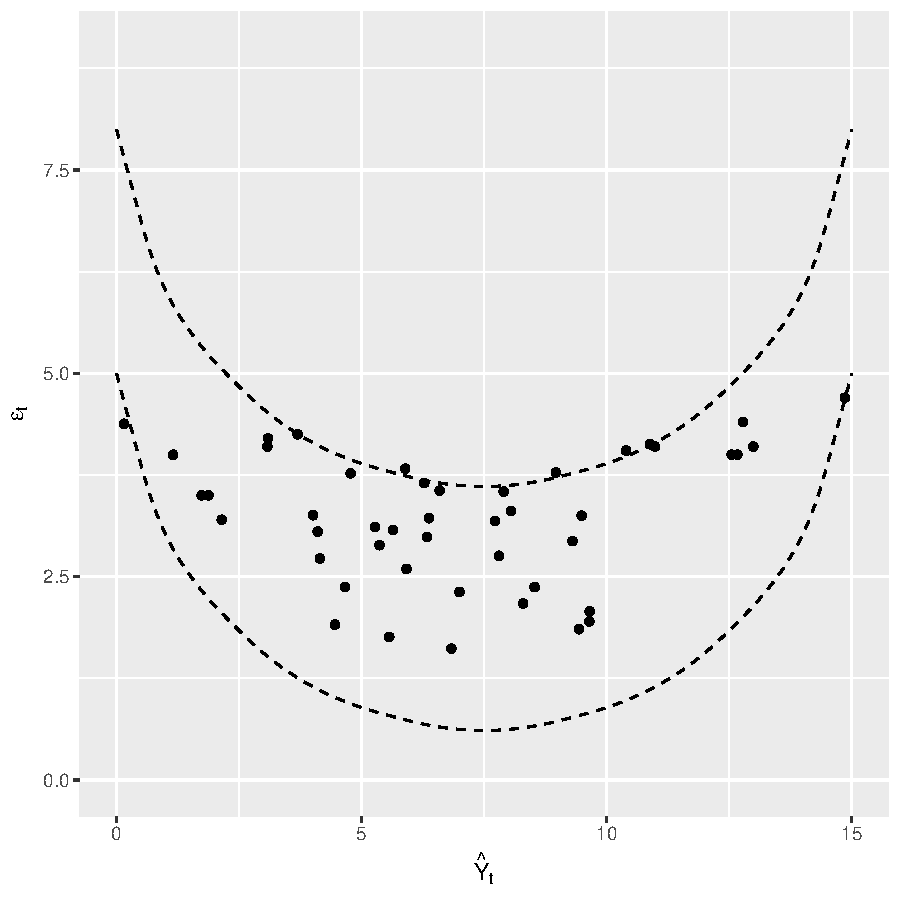
\includegraphics{notes_de_cours-033}

\subsubsection{Distribution \emph{conique}}
Cette distribution des résidus semble suivre être distribuer dans un cone. La variance n'est probablement pas constante. Il y a violation de l'hypothèse \ref{post2}. 

\bigskip
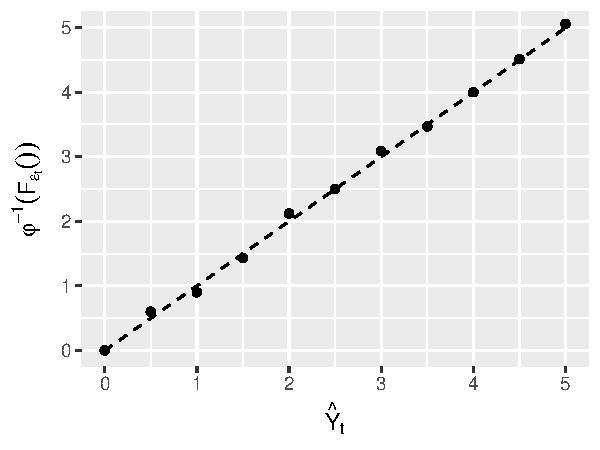
\includegraphics{notes_de_cours-034}

\subsection{Quantiles normaux}
On appel parfois le diagramme Quantile-Quantile ou Q-Q plot. Il s'agit d'un outil permettant d'évaluer la pertinence de l'ajustement d'une distribution. \newline

On ajuste selon une loi normale la fonction empirique des résidus par rapport aux résidus. \newline

On cherche à avoir une droite à $45^\circ$. Dans cette situation, cela signifie $\varepsilon_t \sim N(0,1)$.

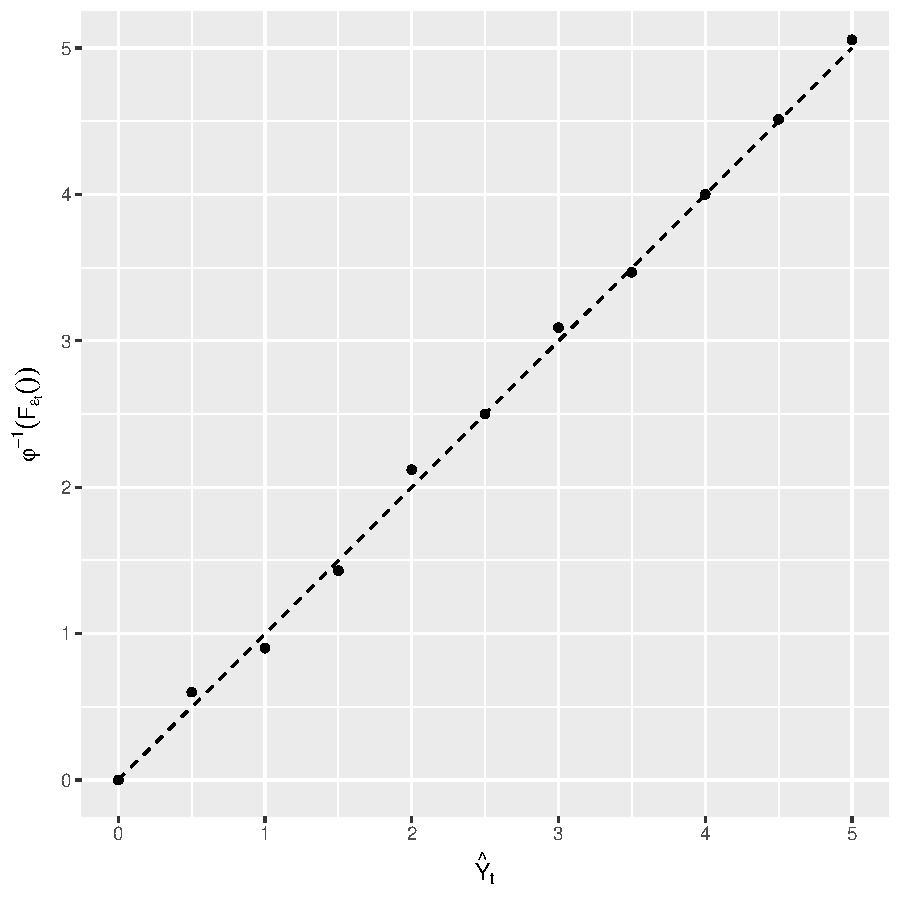
\includegraphics{notes_de_cours-035}

\subsection{Exemple complet}
\label{ex:chapitre3}

On poursuit avec un exemple complet pour synthétiser l'information du chapitre 3. \newline

On reprend le scénario du Titanic de la section \ref{ex:multiple}, cette fois on va utiliser un modèle complet avec des catégories et déterminer le meilleur modèle avec la technique de régression pas à pas \footnote{Le code source complet de l'exemple est disponible à l'annexe \ref{codesour:chap3}}.  \newline

Tout d'abord, voici la signification des variables :
\begin{center}
\begin{tabularx}{\textwidth}{XX}
\hline
Variable & Définition \\
\hline
Survival & Survie du passager au naufrage du Titanic \\
Pclass & Catégorie du billet \\
Sex & Sexe \\
Age & Âge \\
sibsp & Nombre se frères et sœurs / époux à bord du Titanic \\
parch & Nombre de parents / enfants à bord du Titanic \\
ticket & Numéro du billet \\
fare & Prix du billet \\
cabin & Numéro de la cabine \\
embarked & Port d'embarquement \\
\hline
\end{tabularx}
\end{center}

L'étape suivante consiste à analyser notre jeu de donnée et de retirer les variables inutiles:
\begin{Schunk}
\begin{Soutput}
  PassengerId       Survived          Pclass     
 Min.   :  1.0   Min.   :0.0000   Min.   :1.000  
 1st Qu.:223.5   1st Qu.:0.0000   1st Qu.:2.000  
 Median :446.0   Median :0.0000   Median :3.000  
 Mean   :446.0   Mean   :0.3838   Mean   :2.309  
 3rd Qu.:668.5   3rd Qu.:1.0000   3rd Qu.:3.000  
 Max.   :891.0   Max.   :1.0000   Max.   :3.000  
                                                 
                                    Name         Sex           Age       
 Abbing, Mr. Anthony                  :  1   female:314   Min.   : 0.42  
 Abbott, Mr. Rossmore Edward          :  1   male  :577   1st Qu.:20.12  
 Abbott, Mrs. Stanton (Rosa Hunt)     :  1                Median :28.00  
 Abelson, Mr. Samuel                  :  1                Mean   :29.70  
 Abelson, Mrs. Samuel (Hannah Wizosky):  1                3rd Qu.:38.00  
 Adahl, Mr. Mauritz Nils Martin       :  1                Max.   :80.00  
 (Other)                              :885                NA's   :177    
     SibSp           Parch             Ticket         Fare       
 Min.   :0.000   Min.   :0.0000   1601    :  7   Min.   :  0.00  
 1st Qu.:0.000   1st Qu.:0.0000   347082  :  7   1st Qu.:  7.91  
 Median :0.000   Median :0.0000   CA. 2343:  7   Median : 14.45  
 Mean   :0.523   Mean   :0.3816   3101295 :  6   Mean   : 32.20  
 3rd Qu.:1.000   3rd Qu.:0.0000   347088  :  6   3rd Qu.: 31.00  
 Max.   :8.000   Max.   :6.0000   CA 2144 :  6   Max.   :512.33  
                                  (Other) :852                   
         Cabin     Embarked
            :687    :  2   
 B96 B98    :  4   C:168   
 C23 C25 C27:  4   Q: 77   
 G6         :  4   S:644   
 C22 C26    :  3           
 D          :  3           
 (Other)    :186           
\end{Soutput}
\end{Schunk}

\bigskip
Certaine variable ne son d'auncun intérêt pour estimer l'âge d'un passager, tel que :
\begin{itemize}
\item \emph{PassengerId}, car il s'agit d'un numéro unique pour chaque passager. (Max. : 891 pour 891 observations)
\item \emph{Name}, dans son étât actuel le nom du passager n'est pas très utile car il s'agit d'observation unique.
\item \emph{Ticket}, car il s'agit d'un numéro unique pour chaque passager.
\item \emph{SibSP}, \emph{Parch} et \emph{Cabin} sont retirer pour de fins de simplification. 
\end{itemize}

\bigskip
On cherche maintenant à transformer une donnée pour en tirer de l'information. On observe que le nom du passager est unique dans son format actuel, mais avec un peu de manipulation de donnée, il est très facile d'extraire son nom de famille.


\begin{Schunk}
\begin{Sinput}
> # Visualiser les 6 premières observations par catégorie
> head(summary(data$Surname))
\end{Sinput}
\begin{Soutput}
Andersson      Sage    Carter   Goodwin   Johnson    Panula 
        9         7         6         6         6         6 
\end{Soutput}
\end{Schunk}

On obtient ainsi le modèle complet suivant :
\begin{align*}
\text{Âge}_t = \beta_0 + \beta_1 \times \text{Survived}_t + \beta_2 \times \text{Pclass}_t + \beta_3  \times \text{Sex}_t + \beta_4  \times \text{Fare}_t + \beta_5  \times \text{Embarked}_t + \beta_6  \times \text{Surname}_t + \varepsilon_t
\end{align*}

On peut maintenant trouver le meilleur modèle,

\begin{Schunk}
\begin{Sinput}
> fit <- step(lm(Age ~ Survived + Pclass + Sex + Fare + Embarked + Surname, data), 
+             direction = "both")
\end{Sinput}
\begin{Soutput}
Start:  AIC=3796.05
Age ~ Survived + Pclass + Sex + Fare + Embarked + Surname

            Df Sum of Sq    RSS    AIC
- Surname  533     87709 119664 3672.8
- Pclass     1         3  31958 3794.1
- Fare       1        43  31997 3795.0
<none>                    31955 3796.0
- Embarked   2       336  32291 3799.5
- Sex        1       379  32334 3802.5
- Survived   1      2616  34571 3850.2

Step:  AIC=3672.79
Age ~ Survived + Pclass + Sex + Fare + Embarked

            Df Sum of Sq    RSS    AIC
- Embarked   3       664 120328 3670.7
- Sex        1       187 119851 3671.9
<none>                   119664 3672.8
- Fare       1      1574 121238 3680.1
- Survived   1      4062 123726 3694.6
+ Surname  533     87709  31955 3796.0
- Pclass     1     25962 145626 3811.0

Step:  AIC=3670.74
Age ~ Survived + Pclass + Sex + Fare

            Df Sum of Sq    RSS    AIC
- Sex        1       145 120473 3669.6
<none>                   120328 3670.7
+ Embarked   3       664 119664 3672.8
- Fare       1      1747 122075 3679.0
- Survived   1      4200 124528 3693.2
+ Surname  534     88037  32291 3799.5
- Pclass     1     26337 146664 3810.1

Step:  AIC=3669.61
Age ~ Survived + Pclass + Fare

            Df Sum of Sq    RSS    AIC
<none>                   120473 3669.6
+ Sex        1       145 120328 3670.7
+ Embarked   3       623 119851 3671.9
- Fare       1      1850 122323 3678.5
- Survived   1      6913 127386 3707.4
+ Surname  534     87812  32662 3805.7
- Pclass     1     26875 147349 3811.4
\end{Soutput}
\begin{Sinput}
> fit
\end{Sinput}
\begin{Soutput}
Call:
lm(formula = Age ~ Survived + Pclass + Fare, data = data)

Coefficients:
(Intercept)     Survived       Pclass         Fare  
   54.14124     -6.81709     -9.12040     -0.03671  
\end{Soutput}
\end{Schunk}

\bigskip
On observe que le Q-Q plot suivant pour le modèle

\begin{Schunk}
\begin{Sinput}
> # Q-Q plot 
> plot(fit, which=2)
\end{Sinput}
\end{Schunk}
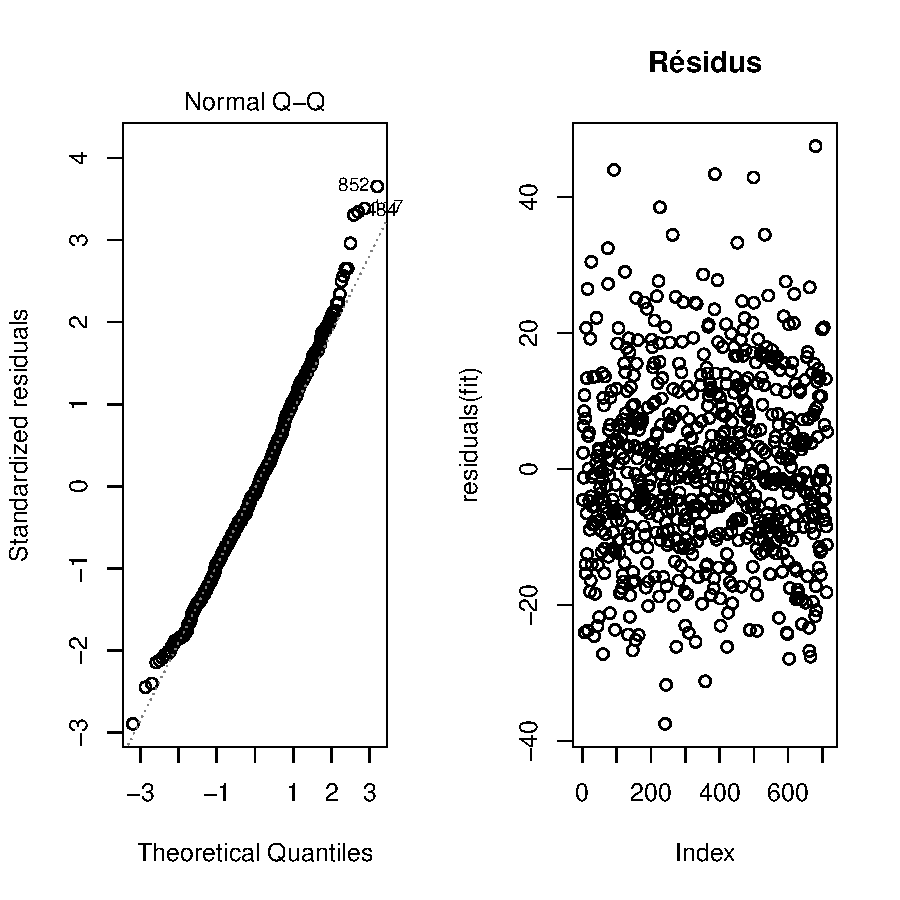
\includegraphics{notes_de_cours-040}

\bigskip
Notre modèle prédit assez bien l'âge, par contre pour des valeurs extrêmes notre prédiction est moins précise. \newline

On va maintenant tester une variable modifier, le log-Fare. En appliquant un log à une valeur numérique, on réduit l'échelle d'écart entre les variables et certaines peuvent mieux prédire après avoir être transformer.

\begin{Schunk}
\begin{Soutput}
Start:  AIC=3796.92
Age ~ Survived + Pclass + Sex + Fare + Embarked + Surname + LogFare

            Df Sum of Sq    RSS    AIC
- Surname  533     84253 116157 3653.6
- Pclass     1         6  31910 3795.0
- LogFare    1        51  31955 3796.0
<none>                    31904 3796.9
- Fare       1        93  31997 3797.0
- Embarked   2       374  32278 3801.2
- Sex        1       409  32313 3804.0
- Survived   1      2614  34518 3851.1

Step:  AIC=3653.56
Age ~ Survived + Pclass + Sex + Fare + Embarked + LogFare

            Df Sum of Sq    RSS    AIC
- Sex        1         6 116163 3651.6
- Embarked   3       682 116839 3651.7
- Fare       1       116 116274 3652.3
<none>                   116157 3653.6
- LogFare    1      3507 119664 3672.8
- Survived   1      4214 120372 3677.0
+ Surname  533     84253  31904 3796.9
- Pclass     1     28085 144242 3806.2

Step:  AIC=3651.59
Age ~ Survived + Pclass + Fare + Embarked + LogFare

            Df Sum of Sq    RSS    AIC
- Embarked   3       677 116840 3649.7
- Fare       1       120 116283 3650.3
<none>                   116163 3651.6
+ Sex        1         6 116157 3653.6
- LogFare    1      3687 119851 3671.9
- Survived   1      5931 122094 3685.1
+ Surname  533     83850  32313 3804.0
- Pclass     1     29036 145199 3808.9

Step:  AIC=3649.74
Age ~ Survived + Pclass + Fare + LogFare

            Df Sum of Sq    RSS    AIC
- Fare       1        99 116939 3648.3
<none>                   116840 3649.7
+ Embarked   3       677 116163 3651.6
+ Sex        1         1 116839 3651.7
- LogFare    1      3633 120473 3669.6
- Survived   1      5953 122794 3683.2
- Pclass     1     29179 146019 3806.9
+ Surname  534     84180  32660 3807.6

Step:  AIC=3648.35
Age ~ Survived + Pclass + LogFare

            Df Sum of Sq    RSS    AIC
<none>                   116939 3648.3
+ Fare       1        99 116840 3649.7
+ Embarked   3       656 116283 3650.3
+ Sex        1         2 116937 3650.3
- LogFare    1      5384 122323 3678.5
- Survived   1      5953 122892 3681.8
- Pclass     1     29081 146021 3804.9
+ Surname  534     84275  32664 3805.7
\end{Soutput}
\begin{Soutput}
Call:
lm(formula = Age ~ Survived + Pclass + LogFare, data = data)

Coefficients:
(Intercept)     Survived       Pclass      LogFare  
     69.419       -6.354      -11.201       -4.060  
\end{Soutput}
\end{Schunk}
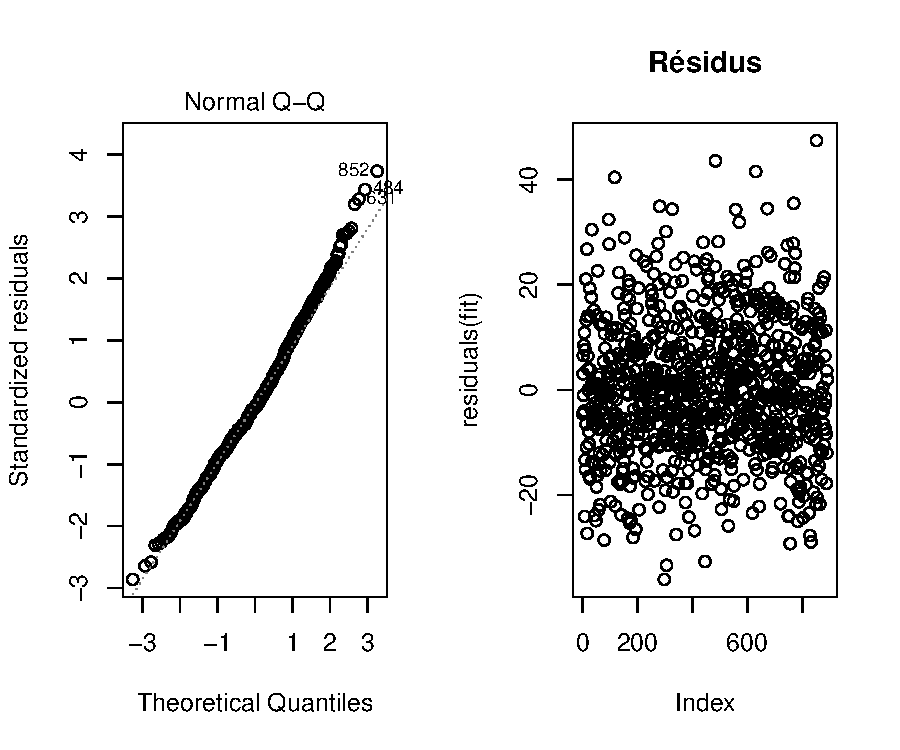
\includegraphics{notes_de_cours-041}

On obtient une légère amélioration de notre modèle et on retient ce modèle. \newline

On cherche maintenant à prédire à partir d'un autre échantillon des données.

\begin{Schunk}
\begin{Sinput}
> head(predict(fitL, dataTest))
\end{Sinput}
\begin{Soutput}
       1        2        3        4        5        6 
21.10578 21.56033 37.79596 27.04870 19.27570 20.43965 
\end{Soutput}
\end{Schunk}

\begin{moreInfo}{\emph{Segmentation des données}}
      En analyse des données, il est primordial de fragmenter les données. On utilise habituellement réduit l'algorithme suivant :
      \begin{enumerate}
      \item 80 \% des données pour l'entraînement (training) et 20 \% pour le test (testing);
      \item 80 \% des données de test pour l'entraînement  (training) et 20 \% pour la validation (validation). 
      \end{enumerate}
      On segmente les données afin d'éviter le surapprentissage (overfitting). Il s'agit de la situation ou toutes les situations possibles sont incluses dans le modèle et celui-ci perd de la qualité prédictive. 
      Dans le cadre du cours, seulement l'étape 1 est suffisante. \newline
      
      Des méthodes plus \href{https://fr.wikipedia.org/wiki/Validation_croisée}{élaborée} et complexe existent pour les données massives et l'apprentissage automatique.
\end{moreInfo}

\chapter{Les modèles linéaires généralisés}
\section{Introduction}
Le modèle de régression linéaire multiple étudié lors des derniers chapitres peut parfois avoir certaines limitations : 
\begin{itemize}
\item On suppose une distribution normale. Dans la plupart des contextes, cette distribution est innaproprié car elle permet des valeurs négatives. On comprend qu'en actuariat, cette situation n'est pas désirable.
\item Hypothèse contraignante de variance constante.
\item Le domaine des variables réponses permet des valeurs entre $-\infty$ et $\infty$. Plusieurs contexte ne se retrouve que dans un domaine non négatifs. De plus, certaine situation pourrait être une variable réponse discrète.
\end{itemize}

Le modèle linéaire généralisé, parfois appeler GLM pour \emph{Generalized Linear Models}, est une généralisation de la régression linéaire multiple dont l'objectif est de palier aux limitations précédentes.

\begin{moreInfo}{\emph{Reformulation}}
     On peut voir le GLM comme une généralisation souple de la régression linéaire. Cette généralisation de la régression linéaire permet au modèle linéaire d'être relié aux variables réponses via une fonction de lien. De plus, le GLM autorise l'amplitude de la variance de chaque mesure en étant une fonction de sa valeur prévue.
\end{moreInfo}

\section{Notions préliminaires : La famille exponentielle}
De manière générale, une variable aléatoire y obéit à une distribution faisant partie de la famille exponentielle si :
\begin{align*}
f_Y(y) &= \exp\bigg\lbrace \frac{y \times \theta - b(\theta)}{a(\phi)} - c(y, \phi) \bigg\rbrace \\
\text{; où } 
\end{align*}
\begin{itemize}
     \item $\theta$ : Paramètre canonique
     \item $\phi $ : Paramètre de dispersion
     \item $a(\phi), b(\theta)$ et $c(y, \phi)$ : 3 fonctions générales de $y, \theta$ et $\phi$.
\end{itemize}

\subsection{Loi Normale}
En posant,
\begin{itemize}
     \item $\theta = \mu$
     \item $\phi = \sigma^2$
     \item $b(\theta) = \frac{\theta^2}{2}$
     \item $a(\phi) = \phi$
     \item $c(y, \phi) = \frac{-1}{2}\bigg(\frac{y^2}{\sigma^2} + \ln(2 \pi \sigma^2) \bigg)$
     \item[] alors,
     \begin{align*}
          f_Y(y) &= \frac{1}{\sqrt{2 \pi \sigma^2}}e^{\frac{-1}{2}\times \big(\frac{y - \mu}{\sigma} \big)^2}
     \end{align*}
     \item[] et
     \begin{align*}
          Y \sim N(\mu, \sigma^2)
     \end{align*}
\end{itemize}

\subsubsection*{Preuve}
\begin{align*}
f_Y(y) &= \exp\Bigg\lbrace \frac{y \times \mu - \frac{\mu^2}{2}}{\sigma^2} + \frac{-1}{2} \bigg( \frac{y^2}{\sigma^2} + \ln(2 \pi \sigma^2) \bigg) \Bigg\rbrace \\
&= \exp\Bigg\lbrace \frac{-y^2}{2\sigma^2} + \frac{y \times \mu}{\sigma^2} - \frac{\mu^2}{2\sigma^2} - \frac{\ln(2 \pi \sigma^2)}{2} \Bigg\rbrace \\
&= \exp\Bigg\lbrace \frac{-1}{2\sigma^2}(y - \mu)^2 - \frac{1}{2} \ln(2\pi \sigma^2)\Bigg\rbrace \\
&= \frac{1}{\sqrt{2 \pi \sigma^2}}e^{\frac{-1}{2}\times \big(\frac{y - \mu}{\sigma} \big)^2}
\end{align*}

\subsection{Loi Poisson}
En posant,
\begin{itemize}
     \item $\theta = \ln(\mu)$
     \item $\phi = 1$
     \item $b(\theta) = e^{\theta}$
     \item $a(\phi) = \phi$
     \item $c(y, \phi) = -\ln(\fact{y})$
     \item[] alors,
     \begin{align*}
          f_Y(y) &= \frac{e^{-\mu}\mu^y}{\fact{y}}
     \end{align*}
     \item[] et
     \begin{align*}
          Y \sim \text{Poisson}(\mu)
     \end{align*}
\end{itemize}

\subsubsection*{Preuve}
\begin{align*}
f_Y(y) &= \exp\Bigg\lbrace \frac{y \ln(\mu) - e^{\ln(\mu)}}{1} + (-1) \ln(\fact{y}) \Bigg\rbrace \\
&= \exp\Bigg\lbrace y \ln(\mu) - \mu + \ln(\frac{1}{\fact{y}}) \Bigg\rbrace \\
&= \frac{e^{-\mu}\mu^y}{\fact{y}}
\end{align*}

\subsection{Loi Bernouilli}
En posant,
\begin{itemize}
     \item $\theta = \ln(\frac{\pi}{(1 -\pi)})$
     \item $\phi = 1$
     \item $b(\theta) = \ln(1 + e^{\theta})$
     \item $a(\phi) = \phi$
     \item $c(y, \phi) = \emptyset$
     \item[] alors,
     \begin{align*}
          f_Y(y) &= \pi^y \times (1 - \pi)^{1 - y}
     \end{align*}
     \item[] et
     \begin{align*}
          Y \sim \text{Bern}(\pi)
     \end{align*}
\end{itemize}

\subsubsection*{Preuve}
\begin{align*}
f_Y(y) &= \exp\Bigg\lbrace \frac{y \times \ln\big(\frac{\pi}{(1 -\pi)}\big) - \ln\big( 1 + e^{\ln\big(\frac{\pi}{(1 -\pi)}\big)}\big)}{1} + 0 \Bigg\rbrace \\
&= \exp\Bigg\lbrace y \times \ln(\pi) - y \ln(1 -\pi) + \ln( 1 -\pi) \Bigg\rbrace \\
&= \exp\Bigg\lbrace y \times \ln(\pi) + (1 - y) \ln(1 -\pi) \Bigg\rbrace \\
&= \pi^y \times (1 - \pi)^{1 - y}
\end{align*}

\subsection{Autres lois}
\begin{itemize}
\item Loi beta
\item Loi binomiale
\item Loi gamma
\item Loi inverse-Gaussienne
\item Loi binomiale négative
\item Loi pareto
\item Loi weibull
\end{itemize}

sont aussi des distributions qui appartiennent à la famille exponentielle.

\section{Généralités sur les modèles de régression avec la famille exponentielle}

\subsection{Contexte}
Le contexte est très similaire à celui de la régression multiple :
\subsection{Autres lois}
\begin{itemize}
\item $\mathbb{Y}_{n \times 1}$ : Vecteur des observations de $Y_i$, où $i = 1,...,n$.
\item $\mathbb{X}_{n \times (p+1)}$ : Matrice schéma contenant n lignes d'observations et $(p+1)$ colonnes de variables explicatives.
\item $\mathbb{\beta}_{(p+1) \times 1}$ : Vecteur des $(p+1)$ paramètres $\beta_0, \beta_1,...,\beta_p$ à estimer. 
\end{itemize}

\subsection{Structure du modèle}
On suppose maintenant que 
$$
(Y_i|X_i) \sim \text{ Famille exponentielle}
$$
et que
\begin{align*}
g(E[Y_i|X_i]) &= X_i\beta \\
&= \beta_0 + \beta_1X_{i,1} + ... + \beta_pX_{i,p}\\
\end{align*}
où $g(\bullet)$ est une fonction continue appelée une \textbf{fonction de lien}.

\subsection{Propriété de la fonction de lien}
\subsubsection{Domaine de $g(\bullet)$}
Domaine des valeurs possible de $\mu = \varphi(\mu)$ \newline

Voici quelques exemple de domaine de la fonction de lien :
\begin{itemize}
\item Loi gamma $\Rightarrow \varphi(\mu) = [0, \infty[$
\item Loi bernouilli $\Rightarrow \varphi(\mu) = [0, 1]$
\end{itemize}

\subsubsection{Image de $g(\bullet)$}
L'image de la fonction de lien est $\mathbb{R} = ] - \infty, \infty [$

\subsubsection{Conclusion}
Le but de la fonction de lien est d'obtenir des valeurs de $\mu$ qui correspond bien au contexte du modèle à parti du prédicteur linéaire $X_i\beta$ qui peut prendre des valeurs dans $\mathbb{R}$. Autrement dit, on défini un domaine cohérent pour les valeurs réponses et on ne restreint pas les valeurs possibles des observations.\newline

Ainsi, on obtient $\mu$ en inversant $g(\bullet)$ :
\begin{align*}
g(E[Y_i|X_i]) &= X_i\beta \\
\end{align*}
\begin{equation}
\label{eq:fonctionlien}
\color{blue}
\boxed{\color{black}
E[Y_i|X_i] = g^{-1}(X_i\beta]
}
\end{equation}
Il est donc nécessaire de choisir une fonction inversible pour la fonction de lien.

\section{Approche générale}
\subsection{Procédure avec les GLM}
\begin{itemize}
\item Choisir une distribution pour $Y$ dans la famille exponentielle.
\item Choisir une fonction de lien $g(\bullet)$.
\item Estimer les paramètres $\utilde{\beta}$ et $\phi$.
\item Valider le modèle.
\end{itemize}

\subsection{Estimation des paramètres}
Dans le cas des GLM, on estime les paramètres en utilisant la méthode du maximum de vraisemblance. \newline

On souhaite choisir $\utilde{\beta}$ qui maximise la fonction de vraisemblance suivante qui sera notre nouvelle métrique de distance:
$$
l(\utilde{\beta}) = \sum_{i=1}^n \ln(f_Y(y_i))
$$

En pratique, il est d'usage d'utiliter la méthode de Newton-Raphson pour maximiser numériquement $l(\utilde{\beta})$. \newline

Pour ce faire, on pose $\hat{\utilde{\beta}}^{(k)}$, le vecteur contenant les valeurs estimés pour $\utilde{\beta}$ après la $k^e$ itératopm de l'algorithme. \newline

En supposant que l'algorithme ait convergé après l'itération (i+1), alors on a que :
$$
\frac{\partial}{\partial \utilde{\beta}} l(\utilde{\beta}^{(i+1)}) = 0
$$
ou encore que
\begin{equation}
\label{eq:score}
S(\utilde{\beta}^{(i+1)}) = 0
\end{equation}

où $S(\bullet)$ est appelé le vecteur score et est défini ainsi :
$$
S(\utilde{\beta}^{(i+1)}) = 
\begin{bmatrix}
  \frac{\partial}{\partial\beta_0}  l(\utilde{\beta}) \\
  \frac{\partial}{\partial\beta_1}  l(\utilde{\beta}) \\
  \vdots \\
  \frac{\partial}{\partial\beta_p}  l(\utilde{\beta}) \\
\end{bmatrix}_{(p+1) \times 1}
$$

Pour obtenir un algorithme permettant d'obtenir un estimateur récursivement, à partir de $\hat{\utilde{\beta}}^{(i)}$, il faut développer $S(\utilde{\beta}^{(i+1)}) $ autour de $\hat{\utilde{\beta}}^{(i)}$ à l'aide d'une série de Taylor :
\begin{align*}
S(\utilde{\beta}^{(i+1)}) &= S(\utilde{\beta}^{(i)}) + \Bigg[ \frac{\partial}{\partial\utilde{\beta}}(S(\utilde{\beta}^{(i)})) \Bigg]\Bigg(\hat{\utilde{\beta}}^{(i+1)} - \hat{\utilde{\beta}}^{(i)} \Bigg)
\end{align*}
En substituant cette expresion dans l'équation \ref{eq:score}, on obtient le développement suivant:
\begin{align*}
 S(\utilde{\beta}^{(i)}) + \frac{\partial}{\partial\utilde{\beta}}(S(\utilde{\beta}^{(i)})) \Big(\hat{\utilde{\beta}}^{(i+1)} - \hat{\utilde{\beta}}^{(i)} \Big) &= 0
\end{align*}

ou encore,
\begin{align*}
 S(\utilde{\beta}^{(i)}) + (- I(\hat{\utilde{\beta}}^{(i)}))\Big(\hat{\utilde{\beta}}^{(i+1)} - \hat{\utilde{\beta}}^{(i)} \Big) &= 0
\end{align*}

où $I(\utilde{\beta})$ correspond à la matrice d'information de Fisher et est donnée par :
$$
I(\utilde{\beta}) = 
\begin{bmatrix}
  \frac{\partial^2}{\partial\beta_0^2}  l(\utilde{\beta}) & \frac{\partial^2}{\partial\beta_0\partial\beta_1}  l(\utilde{\beta}) & \cdots \frac{\partial^2}{\partial\beta_0\partial\beta_p}  l(\utilde{\beta})\\
  \vdots & \vdots & \vdots\\
  \frac{\partial^2}{\partial\beta_0\partial\beta_p}  l(\utilde{\beta}) & \frac{\partial^2}{\partial\beta_1\partial\beta_p}  l(\utilde{\beta}) & \cdots \frac{\partial^2}{\partial\beta_p^2}  l(\utilde{\beta})\\
\end{bmatrix}_{(p+1) \times (p+1)}
$$
Ainsi, on peut réécrire l'expression de la façon suivante:
\begin{align*}
S(\utilde{\beta}^{(i)}) &= I(\hat{\utilde{\beta}}^{(i)}) \Big(\hat{\utilde{\beta}}^{(i+1)} - \hat{\utilde{\beta}}^{(i)} \Big) \\
I^{-1}(\hat{\utilde{\beta}}^{(i)}) S(\utilde{\beta}^{(i)}) &= \hat{\utilde{\beta}}^{(i+1)} - \hat{\utilde{\beta}}^{(i)} \\
\end{align*}

\begin{equation}
\label{eq:glmbeta}
\color{blue}
\boxed{\color{black}
\hat{\utilde{\beta}}^{(i+1)} = \hat{\utilde{\beta}}^{(i)} + I^{-1}(\hat{\utilde{\beta}}^{(i)}) S(\utilde{\beta}^{(i)})
}
\end{equation}
Cette équation correspond à 
\begin{align*}
\text{Vecteur de paramètre mis à jour} &= \text{Ancien vecteur de paramètre} \\
&+ \text{Produit matriciel entre l'inverse de la  matrice Fisher et le vecteur score}
\end{align*}

\subsection{Validation \emph{global} du modèle avec la \emph{déviance}}
En réécrivant la fonction de vraisemblance $l(\utilde{\beta})$ comme suit :
\begin{align*}
l(\utilde{\beta}) &= \sum_{i=1}^n \ln(f_Y(y_i)) \\
&= \sum_{i=1}^n \ln(f_Y(y_i; \mu_i)) \text{ ; où } \mu_i = g^{-1}(X_i \utilde{\beta}) \\
&= l(\utilde{y}, \utilde{\beta}) \\
\end{align*}
On peut définir la statistique de déviance $D(\utilde{\beta})$ comme suit :

\begin{align*}
D(\utilde{\beta}) &= 2 \times \Big( \underbrace{l(\utilde{y}, \utilde{y})} - \underbrace{l(\utilde{y}, \utilde{\beta})} \Big) \\ 
& \text{Log vraissemblance} \text{Log vraissemblance} \\
& \text{sous un modèle parfait}  \text{du modèle obtenu} \\
\end{align*}

\begin{center}
\begin{tabularx}{\textwidth}{cXX}
$D(\utilde{\beta})$ &= $2 \times \Big( \underbrace{l(\utilde{y}, \utilde{y})}$ & $- \underbrace{l(\utilde{y}, \utilde{\beta})} \Big)$ \\
& Log vraissemblance \newline sous un modèle parfait & Log vraissemblance \newline du modèle obtenu\\
\end{tabularx}
\end{center}

On remarque que dans le cas de la famille exponentielle, on aura 

\begin{equation}
\label{eq:deviance}
\color{blue}
\boxed{\color{black}
D(\utilde{\beta}) = 2 \times \sum_{i=1}^n \Big\lbrace y_i \times \big( \theta(y_i) - \theta(\mu_i) \big) - b(\theta(y_i)) + b(\theta(\mu_i)) \Big\rbrace
}
\end{equation}

\subsubsection{Loi normale}
\begin{align*}
D(\utilde{\beta}) &= 2 \times \sum_{i=1}^n \Big\lbrace y_i (y_i - \mu_i) - \frac{y_i^2}{2} + \frac{\mu_i^2}{2} \Big\rbrace \\
&= \sum_{i=1}^n \Big\lbrace 2y_i^2 - y_i\times\mu_i - y_i^2 + \mu_i^2 \Big\rbrace \\
&= \sum_{i=1}^n \Big\lbrace y_i^2 - 2y_i\times\mu_i  + \mu_i^2 \Big\rbrace \\
&= \sum_{i=1}^n (y_i - \mu_i)^2\\
&= \sum_{i=1}^n \varepsilon_t^2\\
&= SSE
\end{align*}
\subsubsection*{Conclusion}
Dans le cas de la loi Normale, la déviance est égale à SSE. \newline

De ce fait, $D(\utilde{\beta})$ constitue une généralisation de SSE qui sera valide avec toutes les sous-cas de la famille exponentielle.

\subsubsection{Loi de Poisson}
\begin{align*}
D(\utilde{\beta}) &= 2 \times \sum_{i=1}^n \Big\lbrace y_i \ln\big( \frac{y_i}{\mu_i}\big) - (y_i - \mu_i) \Big\rbrace \\
&\neq SSE
\end{align*}

\subsubsection{Loi binomiale$(m_i, \mu_i)$}
\begin{align*}
D(\utilde{\beta}) &= 2 \times \sum_{i=1}^n \Big\lbrace y_i \ln\big( \frac{y_i}{\mu_i}\big) + (m_i - y_i)\times \ln\big( \frac{m_i - y_i}{m_i - \mu_i}\big) \Big\rbrace \\
&\neq SSE
\end{align*}

\subsubsection{Loi gamma}
\begin{align*}
D(\utilde{\beta}) &= 2 \times \sum_{i=1}^n \Big\lbrace -\ln\big( \frac{y_i}{\mu_i}\big) + \frac{y_i - \mu_i}{\mu_i} \Big\rbrace \\
&\neq SSE
\end{align*}

\subsubsection{Loi inverse Gausienne}
\begin{align*}
D(\utilde{\beta}) &= \times \sum_{i=1}^n \frac{(y_i - \mu_i)^2}{\frac{\mu_i^2}{y_i}}\\
&\neq SSE
\end{align*}

\subsubsection*{Conclusion}
La déviance correspond à SSE seulement pour la distribution Normale. Dans les autres cas, on a une mesure plus générale.

\subsection{Validation \emph{local} du modèle avec des tests d'hypothèses et intervalles de confiances}

%%%%%%%% Annexe %%%%%%%%%%%%%%%%%%%%%%%%
\newpage

\appendix

\chapter{Code source de l'exemple chapitre 3}
\label{codesour:chap3}
(Section \ref{ex:chapitre3})

\begin{lstlisting}[linerange=\\begin\{Sinput\}-\\end\{Sinput\},includerangemarker=false, caption = Code source en R pour l'exemple]
\begin{Schunk}
\begin{Sinput}
> # Import data
> data <- read.csv('data/Titanic/train.csv', stringsAsFactors = T)
> summary(data)
> # Ajout de la variable nom de famille
> data$Surname <- as.factor(sapply(as.character(data$Name),  
+                        function(x) strsplit(x, split = '[,]')[[1]][1]))
> # Modele de regression stepwise
> fit <- step(lm(Age ~ Survived + Pclass + Sex + Fare + Embarked + Surname, data), direction = "both")
> fit
> # Q-Q plot 
> plot(fit, which=2)
> # Ajout de la variable Log - Fare
> data$LogFare <- log(data$Fare)
> data$LogFare[data$LogFare == -Inf] <- 0
> fitL <- step(lm(Age ~ Survived + Pclass + Sex + Fare + Embarked + Surname + LogFare, data), direction = "both")
> fitL
> # Import data
> dataTest <- read.csv('data/Titanic/test.csv', stringsAsFactors = T)
> head(predict(fitL, dataTest))
\end{Sinput}
\end{Schunk}
\end{lstlisting}

\end{document}
